\documentclass[french]{article}
\usepackage[table, dvipsnames]{xcolor}
\usepackage[utf8]{inputenc}
\usepackage{longtable}
% packages possiblement utiles pour un tableau
\usepackage{natbib}
\usepackage[french]{babel}
\usepackage[T1]{fontenc}
\usepackage{graphicx,import}
\usepackage{caption}
\usepackage{booktabs}
\usepackage{changepage}
\usepackage{comment}
\usepackage{geometry}
\usepackage[hidelinks]{hyperref}
\usepackage{titlesec}
\usepackage{subcaption}
\newcommand{\sectionbreak}{\clearpage} % avec titlesec
\geometry{hmargin=2.5cm,vmargin=3cm} % avec geometry

% \hyperref[label]{Nom Clickable~\ref*{label}} met un lien clickable avec le nom "Nom Clickable" vers le label "label" correspondant



\title{Projet d'année - L-Type}
\author{Marco Luyckx, Tiago Marques Correia, Idiatou Diallo, Samed Tektas,
\\Victor Piryns, Alexandre De Groodt, Attilio Discepoli, 
\\Edgardo Cuellar Sanchez, Diego Benitez Alberdi}
\date{2020-2021}

\begin{document}
\maketitle
\begin{center}
    
\includegraphics[scale=0.2]{assets/ULB.png}
\end{center}
\newpage
\tableofcontents
\pagebreak
\section{Introduction}
\subsection{Présentation du projet}
Le projet a pour but de créer un jeu "shoot them up" multijoueur local nommée "L-type".
\newline
\\Tout utilisateur doit posséder un compte pour pouvoir avoir accès aux différentes fonctionnalités du jeu. Une fois le compte créé, l’utilisateur peut se connecter et par après créer ou rejoindre une partie, gérer une liste d’amis, consulter la liste des scores et gérer son compte.
Une partie peut accueillir un à deux joueurs.
Durant le déroulement d’une partie, les joueurs doivent parcourir plusieurs niveaux en détruisant les ennemis qui se présentent devant eux ainsi qu'en esquivant leurs tirs. Les vaisseaux dirigés par les joueurs peuvent récupérer des bonus d’armement lâchés par leurs nombreux adversaires.
\newline
\\Lorsqu’il y a deux joueurs dans une partie, la mort d’un des joueurs n’entraîne pas la fin de la partie, en d’autres mots la partie continue tant qu’un joueur possède encore plus d'un point de vie. Lorsqu’il n’y a qu’un seul joueur, la partie se termine lors de la mort du joueur.
En résumé, le jeu L-Type est un Shoot'em up en scrolling vertical avec la possibilité de jouer en multijoueur local. Chaque joueur peut créer un compte.
\newline
\\Avant chaque partie, le joueur pourra modifier les paramètres de la partie qui va se dérouler (vitesse des ennemis, probabilité de power up,  etc.) mais pas pendant la partie ! Trois niveaux de difficulté sont proposés au(x) joueur(s), chaque niveau étant plus dur que le précédent.
\newline
\\ Un leaderboard permet de consulter les différents scores.

\subsection {Glossaire}
\begin{itemize}
    \item Pseudo: Pseudonyme d'un joueur
    \item Client: Machine du joueur
    \item Serveur: Machine gérant la logistique du jeu (transparent au joueur) 
    \item HUD: "Head-up display" Ensemble d'informations en haut de l'écran renseignant le joueur sur son état  
    \item Room: Salle d'attente avant le début d'une partie
    \item Interpolation: %TODO (note from Victor) proofread
    L'application d'une interpolation linéaire ou sphérique sur un vecteur en visant à rapprocher le vecteur en question à un vecteur cible de X\%, X étant le "poids" de l'interpolation. (Exemple: un vecteur (1,1) avec un vecteur cible (2,2), après interpolation avec un poids de 0.5 (=50\%) sera égal au vecteur (1.5, 1.5))
    \item Pipe: Canal de communication entre le client et le serveur.
    \item Commande: Structure reprenant les actions a effectuer par l'autre processus.
    \item Spawner: Apparition d'entité 
    \item Ship: Vaisseau
    \item Power up: Objet (bonus) lâché par un ennemi lors de sa mort
    \item Leaderboard: Tableau d'affichage des scores.
    \item Enumeration: Type de données consistant en un ensemble de valeurs constantes.
    \item Sérialisation: Codage d'une information sous la forme d'une suite d'informations plus petites.
    \item Structure: Regroupement de données.
    \item Friendly fire: Lorsque les tirs alliés et les collisions entre les joueurs sont activés.
    \item Like: Système de "j'aime" pour les niveaux du jeu. 
    \item SFML: Librairie utilisée pour coder la version graphique du jeu.
    \item Ncurses: Librairie utilisée pour coder la version du jeu en terminal.
    \item VFX: effets visuels.
    \item Frame: Une étape d'animation du jeu,un instant du jeu.\newline\newline
    
    
\end{itemize}
\subsection {Historique de modification}

\begin{center}
\begin{tabular}{ |c|c|c|c|c| } 
\hline
Date & Version & Personnes & Modification  \\
\hline
% -- pour ajouter une ligne, copier la ligne précédente et changer les champs
21.11 & 0.1 & Alexandre & Diagrammes Use Case et tables \\
29.11 & 0.2 & Tout le groupe & Diagrammes de classes \\
04.12 & 0.3 & Idiatou et Attilio & Ajout Glossaire, Introduction et Besoins Utilisateurs \\ 
06.12 & 0.4 & Tout le groupe & Diagrammes de séquences \\
11.12 & 0.5 & Tout le groupe & Ajout des Besoins Système \\ 
14.12 & 0.6 & Diego, Edgardo et Attilio & Enrichissement des Besoins Utilisateurs \\
15.12 & 0.7 & Alex et Samed & Mise en page, refs, diagrammes, correction ortho \\
15.12 & 0.8 & Victor, Marco, Tiago & Enrichissement des Besoins Système \\
16.12 & 0.9 & Tout le groupe & Correction collective et mise au point \\
18.12 & 0.10 & Tout le groupe & Dernier check du SRD avant la remise \\
02.02 & 1.0 & Tout le groupe & Modification du SRD avec les nouvelles règles \\
04.02 & 1.1 & Tout le groupe & Vérifications des modifications \\ 
26.02 & 1.2 & Samed et Diego & Mise à jour diagrammes de classes\\
28.02 & 1.3 & Samed et Diego & Mise à jour diagrammes de classes + explications Use Case\\
01.03 & 1.4 & Diego          & Modification Besoins Utilisateurs et des Besoins système\\
01.03 & 1.5 & Diego          & Mise à jour diagrammes de classes\\
10.03 & 1.6 & Diego          & Mise à jour des diagrammes, du glossaire, explications commandes\\
17.04 & 1.7 & Diego          & Ajout de screenshots\\
18.04 & 1.8 & Diego          & Mise à jour des diagrammes + nouvelles sections\\
19.04 & 1.9 & Diego          & Mise à jour tableau Use Case + glossaire\\
\hline
\end{tabular}
\end{center}


\section{Comment jouer?}
\subsection {Lancement du jeu}
Avant toute chose, il faut savoir comment lancer et jouer au jeu et pour ce faire, vous aurez besoin d'avoir les librairies de ncurses et sfml, qui sont respectivement libncurses-dev et libsfml-dev, ainsi que de sqlite pour la base de données: libsql3-dev. Pour lancer le jeu vous aurez besoin d'ouvrir un terminal depuis le dossier principal du jeu dans lequel vous allez exécuter les commandes suivantes:
\begin{itemize}
    \item ./build.sh
    \item ./ltype\_game\_server\newline
\end{itemize}

La dernière commande sert à lancer le serveur sur lequel le jeu va tourner. Veillez bien à le laisser tourner en fond.
Ensuite afin d'exécuter le jeu vous aurez besoin d'un second terminal pour faire tourner le client à l'aide de la commande:
\begin{itemize}
    \item ./ltype\_game\_client\newline
\end{itemize}
Pour faire tourner le jeu dans sa version terminal,c-à-d avec la librairie "ncurses". Et:
\begin{itemize}
    \item ./ltype\_game\_client -g\newline
\end{itemize}
Pour le faire tourner dans sa version graphique, avec la librairie "SFML".
\subsection {Les touches pour la version terminal (Ncurses)}
\begin{itemize}
    \item Z, UP\_ARROW    : se déplacer vers l'avant, naviguer dans les menus.
    \item Q, LEFT\_ARROW  : se déplacer vers la gauche, naviguer dans les menus.
    \item S, DOWN\_ARROW  : se déplacer vers le bas, naviguer dans les menus.
    \item D, RIGHT\_ARROW : se déplacer vers la droite, naviguer dans les menus.
    \item ESPACE, ENTER   : tirer en jeu.
    \item P               : mettre pause en jeu.
    \item M               : reprendre la partie en pause.
    \item O               : quitter la partie depuis le menu pause.\newline
\end{itemize}
\subsection {Les touches pour la version graphique (SFML)}
\begin{itemize}
    \item MOUSE           : pour naviguer dans les menus.
    \item Z, UP\_ARROW    : se déplacer vers l'avant J1, J2.
    \item Q, LEFT\_ARROW  : se déplacer vers la gauches J1, J2.
    \item S, DOWN\_ARROW  : se déplacer vers le bas J1, J2.
    \item D, RIGHT\_ARROW : se déplacer vers la droite J1, J2.
    \item ESPACE, ENTER   : tirer en jeu J1, J2.
    \item P               : mettre pause en jeu.
    \item M               : reprendre la partie en pause.
    \item O               : quitter la partie depuis le menu pause.
\end{itemize}

% ----------------------------- Besoins UTILISATEURS ------------------------------------ 
\section{Besoins utilisateur}
\subsection {Besoins fonctionnels}
\subsubsection{Connexion} Il est possible pour l'utilisateur de créer un compte avec mot de passe, un pseudonyme associé s'il n'en a pas encore et une question secrète. Par après il pourra se connecter au jeu à l'aide de ces données. (\textit{cf} \hyperref[use case:connection menu]{Connection menu~\ref*{use case:connection menu}})

\label{besoin-user : menu}
\subsubsection{Menu} Une fois connecté, l'utilisateur se retrouve dans le menu principal et a accès à différents choix d'options: créer une partie, avoir accès à son menu "Social", accéder au "leaderboard" qui regroupera les meilleurs scores de certains joueurs ou bien même "levels" si il joue sous la version graphique du jeu.(\textit{cf} \hyperref[use case:main menu]{Main menu~\ref*{use case:main menu}})

\subsubsection{Sociale} L'utilisateur a accès à un menu "Social" regroupant son profil avec sa liste d'amis, et où il peut de ce fait envoyer et recevoir des demandes d'amis. Il peut aussi éditer son profil et voir ses niveaux créés en version graphique.(\textit{cf} \hyperref[use case:online menu]{Social menu~\ref*{use case:online menu}})

\subsubsection{Jeu} Un joueur peut créer une partie, modifier différents paramètres (résistance des ennemis, nombre de vies des joueurs, ...) et il peut aussi joueur en mode 2 joueurs dans ce cas le deuxième joueur se connecte à son compte ou joue en tant qu'invité.(\textit{cf} \hyperref[use case:game]{Game~\ref*{use case:game}})

\subsubsection{Création de niveaux} Un utilisateur pourra, sous la version graphique(SFML) du jeu, créer ses propres niveaux.Il pourra par la suite jouer ses niveaux et même les niveaux des autres joueurs. Un système de "Like" est aussi disponible, ce qui donne la possibilité de like ses niveaux préférés!(\textit{cf} \hyperref[use case:main menu]{Main menu~\ref*{use case:main menu}})

\subsection{Besoins non-fonctionnels}
%\subsubsection{Déconnexion automatique} Lorsqu'un joueur se déconnecte de la partie, il la perd mais elle continue pour l'autre joueur s'il y en a un. Le joueur déconnecté ne gagnera pas d'expérience et le score n'est pas sauvegardé. Cependant l'autre joueur n'est pas affecté.
\subsubsection{Expérience utilisateur (UX)}
Une interface agréable d'utilisation, un bel agencement des menus et des boutons, pour une utilisation optimale de l'interface.

% ----------------------------- Besoins SYSTEME -------------------------------------------
\section{Besoins système}
\subsection{Besoins fonctionnels}
\subsubsection{Base de données} Une base de données existe pour permettre le stockage des données.  
Elle existe du côté du serveur, se chargeant de lire et d'écrire les données nécessaires pour le lancement/déroulement d'une partie, les options possibles, la gestion des menus et le leaderboard.
\subsubsection{Serveur} 
Le serveur est une instance séparée du jeu, qui contient toutes les fonctionnalités essentielles pour son déroulement correct. Il lit les inputs venant du client, mettant à jour la représentation interne du jeu, résolvant toutes les collisions et renvoyant les nouvelles positions au client. Il peut aussi être utilisé pour interpréter les événements des menus, enregistrer des données dans la base de données et/ou lire à partir de celle-ci. 
Le serveur est un processus qui vit indépendamment du client, sur la même machine.
\subsubsection{Client} 
Le client lit les commandes venant du pipe et modifie les positions des entités dans le jeu pour être une copie parfaite de la version du jeu qui existe sur le serveur. Il est aussi responsable de lire les inputs venant de la méthode d'affichage (stdin ou window-events) et de les envoyer au serveur.\\
Le client a deux modes de visualisation du jeu, ASCII et 2D graphique. Vu que les deux versions doivent être compatibles entre elles, et que les positions sont des flottants, elles seront arrondies pour la version ASCII. La librairie utilisée pour la réalisation des interfaces est Ncurses pour l'affichage sur le terminal.Le nombre de client pouvant tourner en même temps a été limité pour une question de rapidité et d'optimisation, même si le serveur a la capacité d'accepter autant de clients qu'il faut.
%\subsubsection{Réseau} 
%Le client et le serveur communiquent à travers des sockets, qui sont une interface pour la communication entre différentes machines à travers une connexion réseau, même sur internet. Il y a plusieurs protocoles existant pour les sockets, mais le premier aperçu est que le protocole UDP peut-être facilement adapté à nos besoins. (UDP est un protocole où les données sont envoyées sous forme de paquets indépendants de manière non séquentielle, et où il n'y a aucune garantie qu'un paquet arrive à sa destination, par contre ceci peut facilement être évité si un horodatage (timestamp) est ajouté dans l'header du paquet et laisse la responsabilité au client de se mettre à jour le plus tôt possible par rapport aux dernières données du serveur. UDP aussi est plus rapide que TCP, ainsi que d'autres protocoles qui ne sont pas fait pour des jeux comme HTTPS/FTP) 
\subsection{Communications}
Les clients et le serveur communiquent à travers des pipes nommés, qui sont une interface de communication entre différents processus existants sur la même machine. Chaque processus peut écrire des "commandes" sur le pipe pour indiquer à l'autre processus les actions qu'il doit effectuer.
\subsubsection{Matériel Informatique}
L'utilisateur communique par le biais de son clavier pour la version du jeu dans le terminal et avec son clavier et sa souris pour la version GUI.
\subsection{Besoins non fonctionnels} 
\subsubsection{Portabilité} Le code du projet doit être réalisé en C++ et pouvoir s'exécuter sur les machines Linux du bâtiment N.O de l'ULB. 
\subsubsection{Rétro compatibilité} Deux joueurs possédants des versions graphiques différentes du jeu (terminal/GUI) doivent pouvoir jouer ensemble.\\
Ceci peut être réalisé grâce à un grand découpage entre la partie logique du jeu et la partie qui va prendre en compte l'affichage. Le client est un front end pour le jeu, sa seule responsabilité est de lire les inputs, les envoyer au serveur pour effectuer un traitement et après mettre à jour les nouvelles positions/données.
\subsection{Connexion}
Un joueur qui oublie son mot de passe peut le changer grâce au bouton "reset password".
Lors de la création de son compte, le joueur choisit une question secrète de sécurité et créée une réponse à cette question. Pour pouvoir changer son mot de passe, le joueur doit répondre correctement à la question sans limite d'essais.
Une fois que la bonne réponse est trouvée le client proposera alors au joueur de mettre son nouveau mot de passe et de le confirmer.
\subsection{Petite explication pour le menu}
Pour l'affichage du menu, il y a une classe principale qui s'occupe de gérer tous les menus en recevant celui à afficher grâce à un MNAME qui est une énumération contenant les noms des différents menus. Elle s'occupe aussi de gérer les commandes avec le serveur pour les menus afin de faire ce qu'il faut au bon moment.
\newpage 
\section{Diagrammes Use case/Tableaux/Séquence/Classe}
\renewcommand{\arraystretch}{1.5}
% CONNECTION USE CASE BRO --------------------------------------------
\subsection{Connection Menu}
\label{Connection menu}
\centering
%Alex- [!htbp] empêche parfois que l'img se mette n'importe où
\begin{figure}[!htbp]
    \centering
    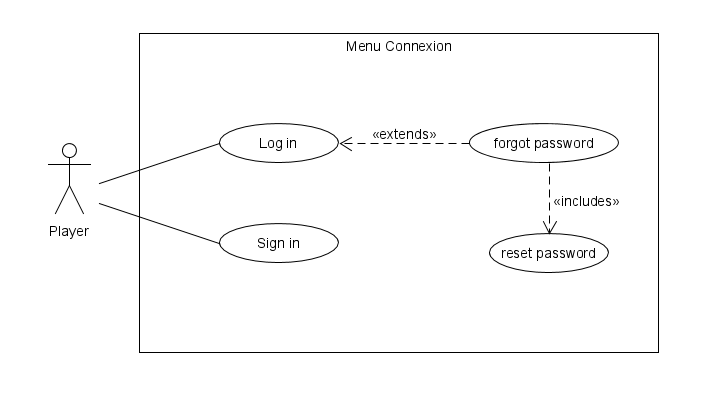
\includegraphics[scale=0.5]{use_case/use_case_connexion.jpg}
    \caption{Diagramme Use Case du menu de connexion}
    \label{use case:connection menu}
\end{figure}

\begin{longtable}{|p{0.17\textwidth}|p{0.17\textwidth}|p{0.17\textwidth}|p{0.17\textwidth}|p{0.17\textwidth}|}
\toprule
\rowcolor{lightgray}
\textbf{Use Case} & \textbf{Pré-conditions} & \textbf{Post-conditions}& \textbf{Cas général} & \textbf{Cas exceptionnels}\\
\midrule
  Sign In & le joueur n'est pas inscrit & le joueur est inscrit et connecté & définir un pseudo, mot de passe et une réponse à la question secrète & le pseudo est déjà utilisé\\
  \hline
  Log In & le joueur est inscrit & le joueur est connecté & il indique le pseudo et le mot de passe qui sont comparés à ceux de la base de donnée & le pseudo/mot de passe ne correspondent pas à ceux de la base de donnée\\
  \hline
  Forgot Password & le joueur est inscrit & entre dans le reset password & il répond à sa question secrète & néant\\
  \hline
  Reset Password & le joueur a bien répondu à la question secrète & le mot de passe du joueur est changé & défini un nouveau mot de passe dans la base de données & néant \\
  \bottomrule
\end{longtable}
\begin{center}
Explication Use Case de Connection Menu : Processus du fonctionnement de la connexion d'un joueur au jeu et de la réinitialisation du mot de passe.
\end{center}

\clearpage
\begin{flushleft}
\subsection{Main Menu}
\end{flushleft}
\begin{figure}[!htbp]
    \centering
    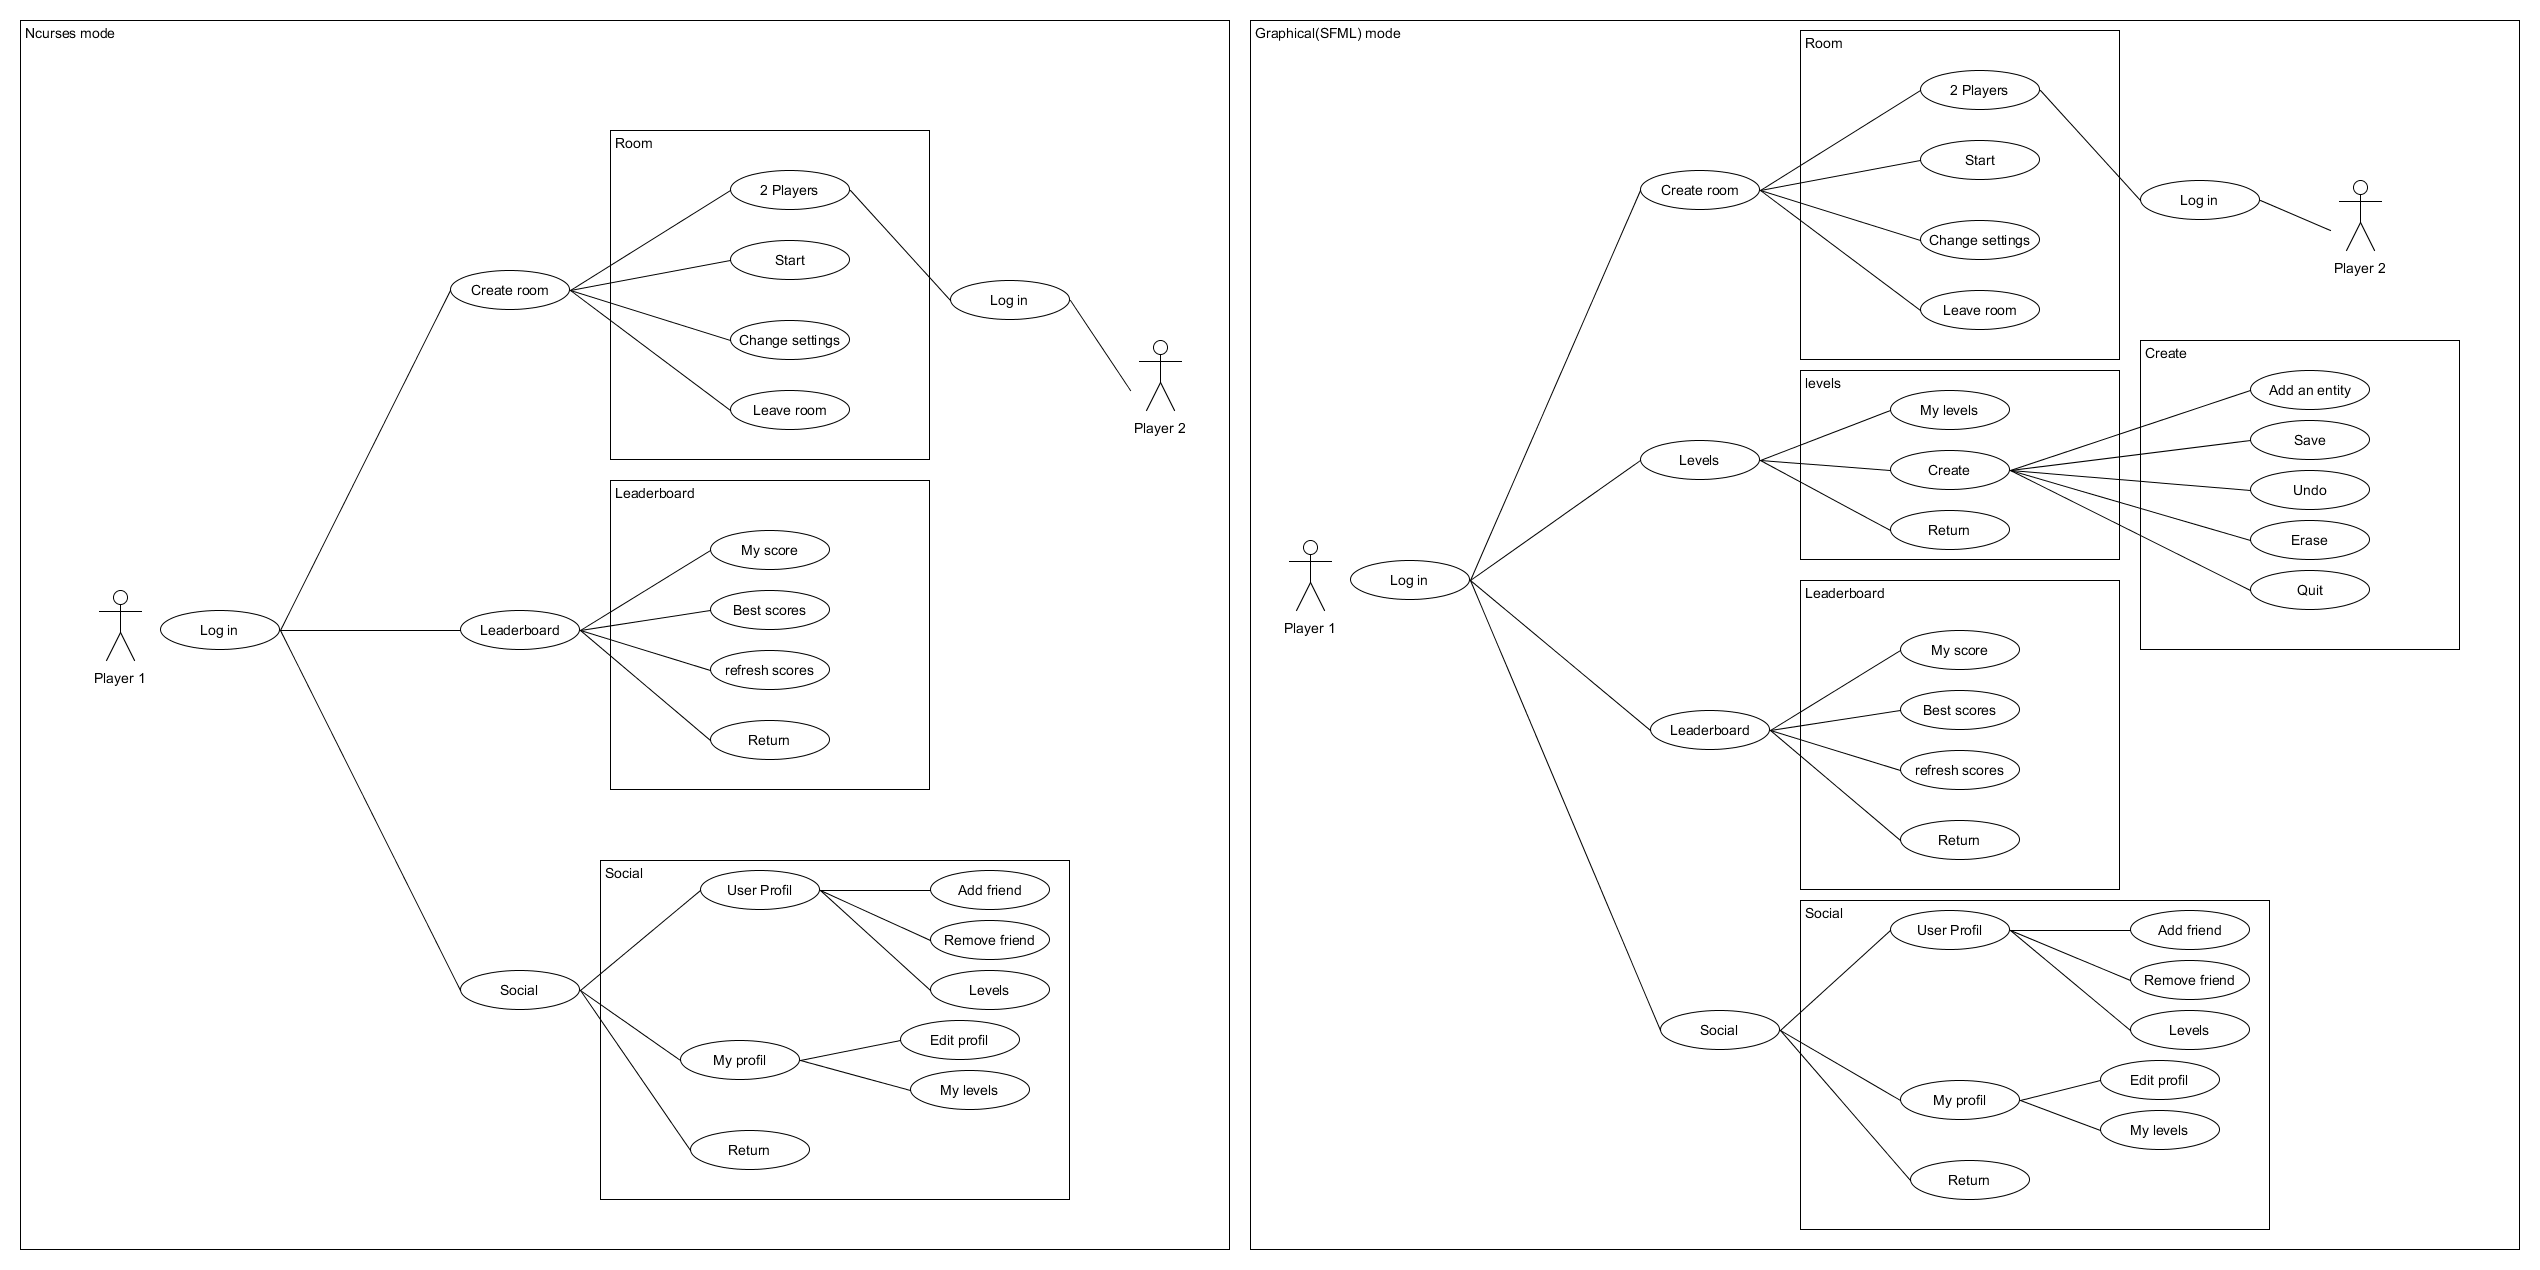
\includegraphics[scale=0.21, angle=90,origin=c]{use_case/use-case-menu.png}
    \caption{Diagramme Use Case du menu}
    \label{use case:main menu}
\end{figure}
\newpage   
\begin{longtable}{|p{0.22\textwidth}|p{0.22\textwidth}|p{0.22\textwidth}|p{0.22\textwidth}|}
  \toprule
  \rowcolor{lightgray}
  \textbf{Use Case} & \textbf{Pré-conditions} & \textbf{Post-conditions}& \textbf{Cas général}\\
  \midrule
  Create Room & néant & est dans une room & changer les settings\\
  \hline
  Levels   & être en partie graphique & est dans le sous menu levels & affiche un second choix de menu \\
  \hline
  Leaderboard & néant & est dans le menu du leaderboard & affiche les scores\\
  \hline
  Social      & néant & est dans le menu "sociale"      & affiche son profil et ses amis\\
  \bottomrule
\end{longtable}
\begin{center}
Explication du Menu : accès aux différents menu; la création d'une partie,le leaderboard et le menu pour le côté sociale.
\end{center}
\begin{flushleft}
\subsection{Room Menu}
\end{flushleft}
\label{use case:room menu}
\begin{longtable}{|p{0.22\textwidth}|p{0.22\textwidth}|p{0.22\textwidth}|p{0.22\textwidth}|}
  \toprule
  \rowcolor{lightgray}
  \textbf{Use Case} & \textbf{Pré-conditions} & \textbf{Post-conditions}& \textbf{Cas général}\\
  \midrule
  Start & néant & est dans une partie qui correspond aux options & jouer seul/à deux\\
  \hline
  Change Settings & player=host & l'option désirée a changé & change un des paramètres: 2 joueus, nombre\de vies, la difficulé, la\ chance d'avoir un bonus\ et le friendly fire\\
  \hline
  Leave & néant & la room n'existe plus et est dans le menu principal & fermer la room et revenir dans le menu principal\\
  \hline
  2 Players & avoir quelqu'un avec qui jouer & est connecté dans la partie & se connecte à son compte ou en créer un\\
  \bottomrule
\end{longtable}
\begin{center}
Explication de Room Menu : Commencer une partie avec un(e) ami(e), changer les paramètres de la partie et de pouvoir quitter le salon.
\end{center}
\newpage
\subsection{Leaderboard}
\label{use case:leaderboard}
\begin{longtable}{|p{0.22\textwidth}|p{0.22\textwidth}|p{0.22\textwidth}|p{0.22\textwidth}|}
  \toprule
  \rowcolor{lightgray}
  \textbf{Use Case} & \textbf{Pré-conditions} & \textbf{Post-conditions}& \textbf{Cas général}\\
  \midrule
  Leaderboard & néant & est dans le leaderboard & affiche le score du jouer et les meilleurs scores\\
  \hline
  my score & a déjà joué & le leaderboard s'affiche & montre constamment son score\\
  \hline
  refresh scores & quelqu'un a joué depuis le dernier refresh & le leaderboard s'est actualisé & met à jour les scores en temps réel.\\
  \hline
  best scores & quelqu'un a déjà joué & le leaderboard s'actualise & montre les meilleurs scores\\
  \hline
  return & néant & est dans le menu principal & retour dans le menu principal\\
  \bottomrule
\end{longtable}
\begin{center}
Explication de Leaderboard : Menu dans lequel nous avons la possibilité de consulter les meilleurs scores réalisés de tout le monde, de ses amis et de soi-même.
\end{center}
\subsection{Social}
\label{use case:Social}
\begin{longtable}{|p{0.22\textwidth}|p{0.22\textwidth}|p{0.22\textwidth}|p{0.22\textwidth}|}
  \toprule
  \rowcolor{lightgray}
  \textbf{Use Case} & \textbf{Pré-conditions} & \textbf{Post-conditions}& \textbf{Cas général}\\
  \midrule
  My profil & néant & est dans son profil & peut éditer son profil,voir ses amis et ses niveaux\\
  \hline
  User profil & a cherché un compte qui existe & le profil s'est affiché  & ajouter ou supprimer l'utilisateur, voir ses niveaux\\
  \hline
  return & néant & est dans le menu principal & retour dans le menu principal\\
  \bottomrule
\end{longtable}
\begin{center}
Explication de Social : Menu dans lequel nous avons la possibilité de consulter son profil, le profil d'un autre joueur, de gérer sa liste d'amis et voir ses niveaux.
\end{center}
\newpage
\subsection{Levels}
\label{use case:Levels}
\begin{longtable}{|p{0.22\textwidth}|p{0.22\textwidth}|p{0.22\textwidth}|p{0.22\textwidth}|}
  \toprule
  \rowcolor{lightgray}
  \textbf{Use Case} & \textbf{Pré-conditions} & \textbf{Post-conditions}& \textbf{Cas général}\\
  \midrule
  My levels & a déjà créé un niveau & voit ses niveaux créés & affiche les niveaux qu'il a créé\\
  \hline
  Create & néant & a créé ou non un niveau  & rentre dans un mode d'édition de niveau\\
  \hline
  return & néant & est dans le menu principal & retour dans le menu principal\\
  \bottomrule
\end{longtable}
\begin{center}
Explication de Levels : Menu où se trouve 2 sous menus, "my levels" qui contient les niveaux créés par l'utilisateur et "create" qui permet de rentrer dans un mode d'édition de niveau.
\end{center}
\newgeometry{vmargin=1.5cm}
\begin{figure}[!htbp] % TODO: note -> SMD TKS
    \centering
    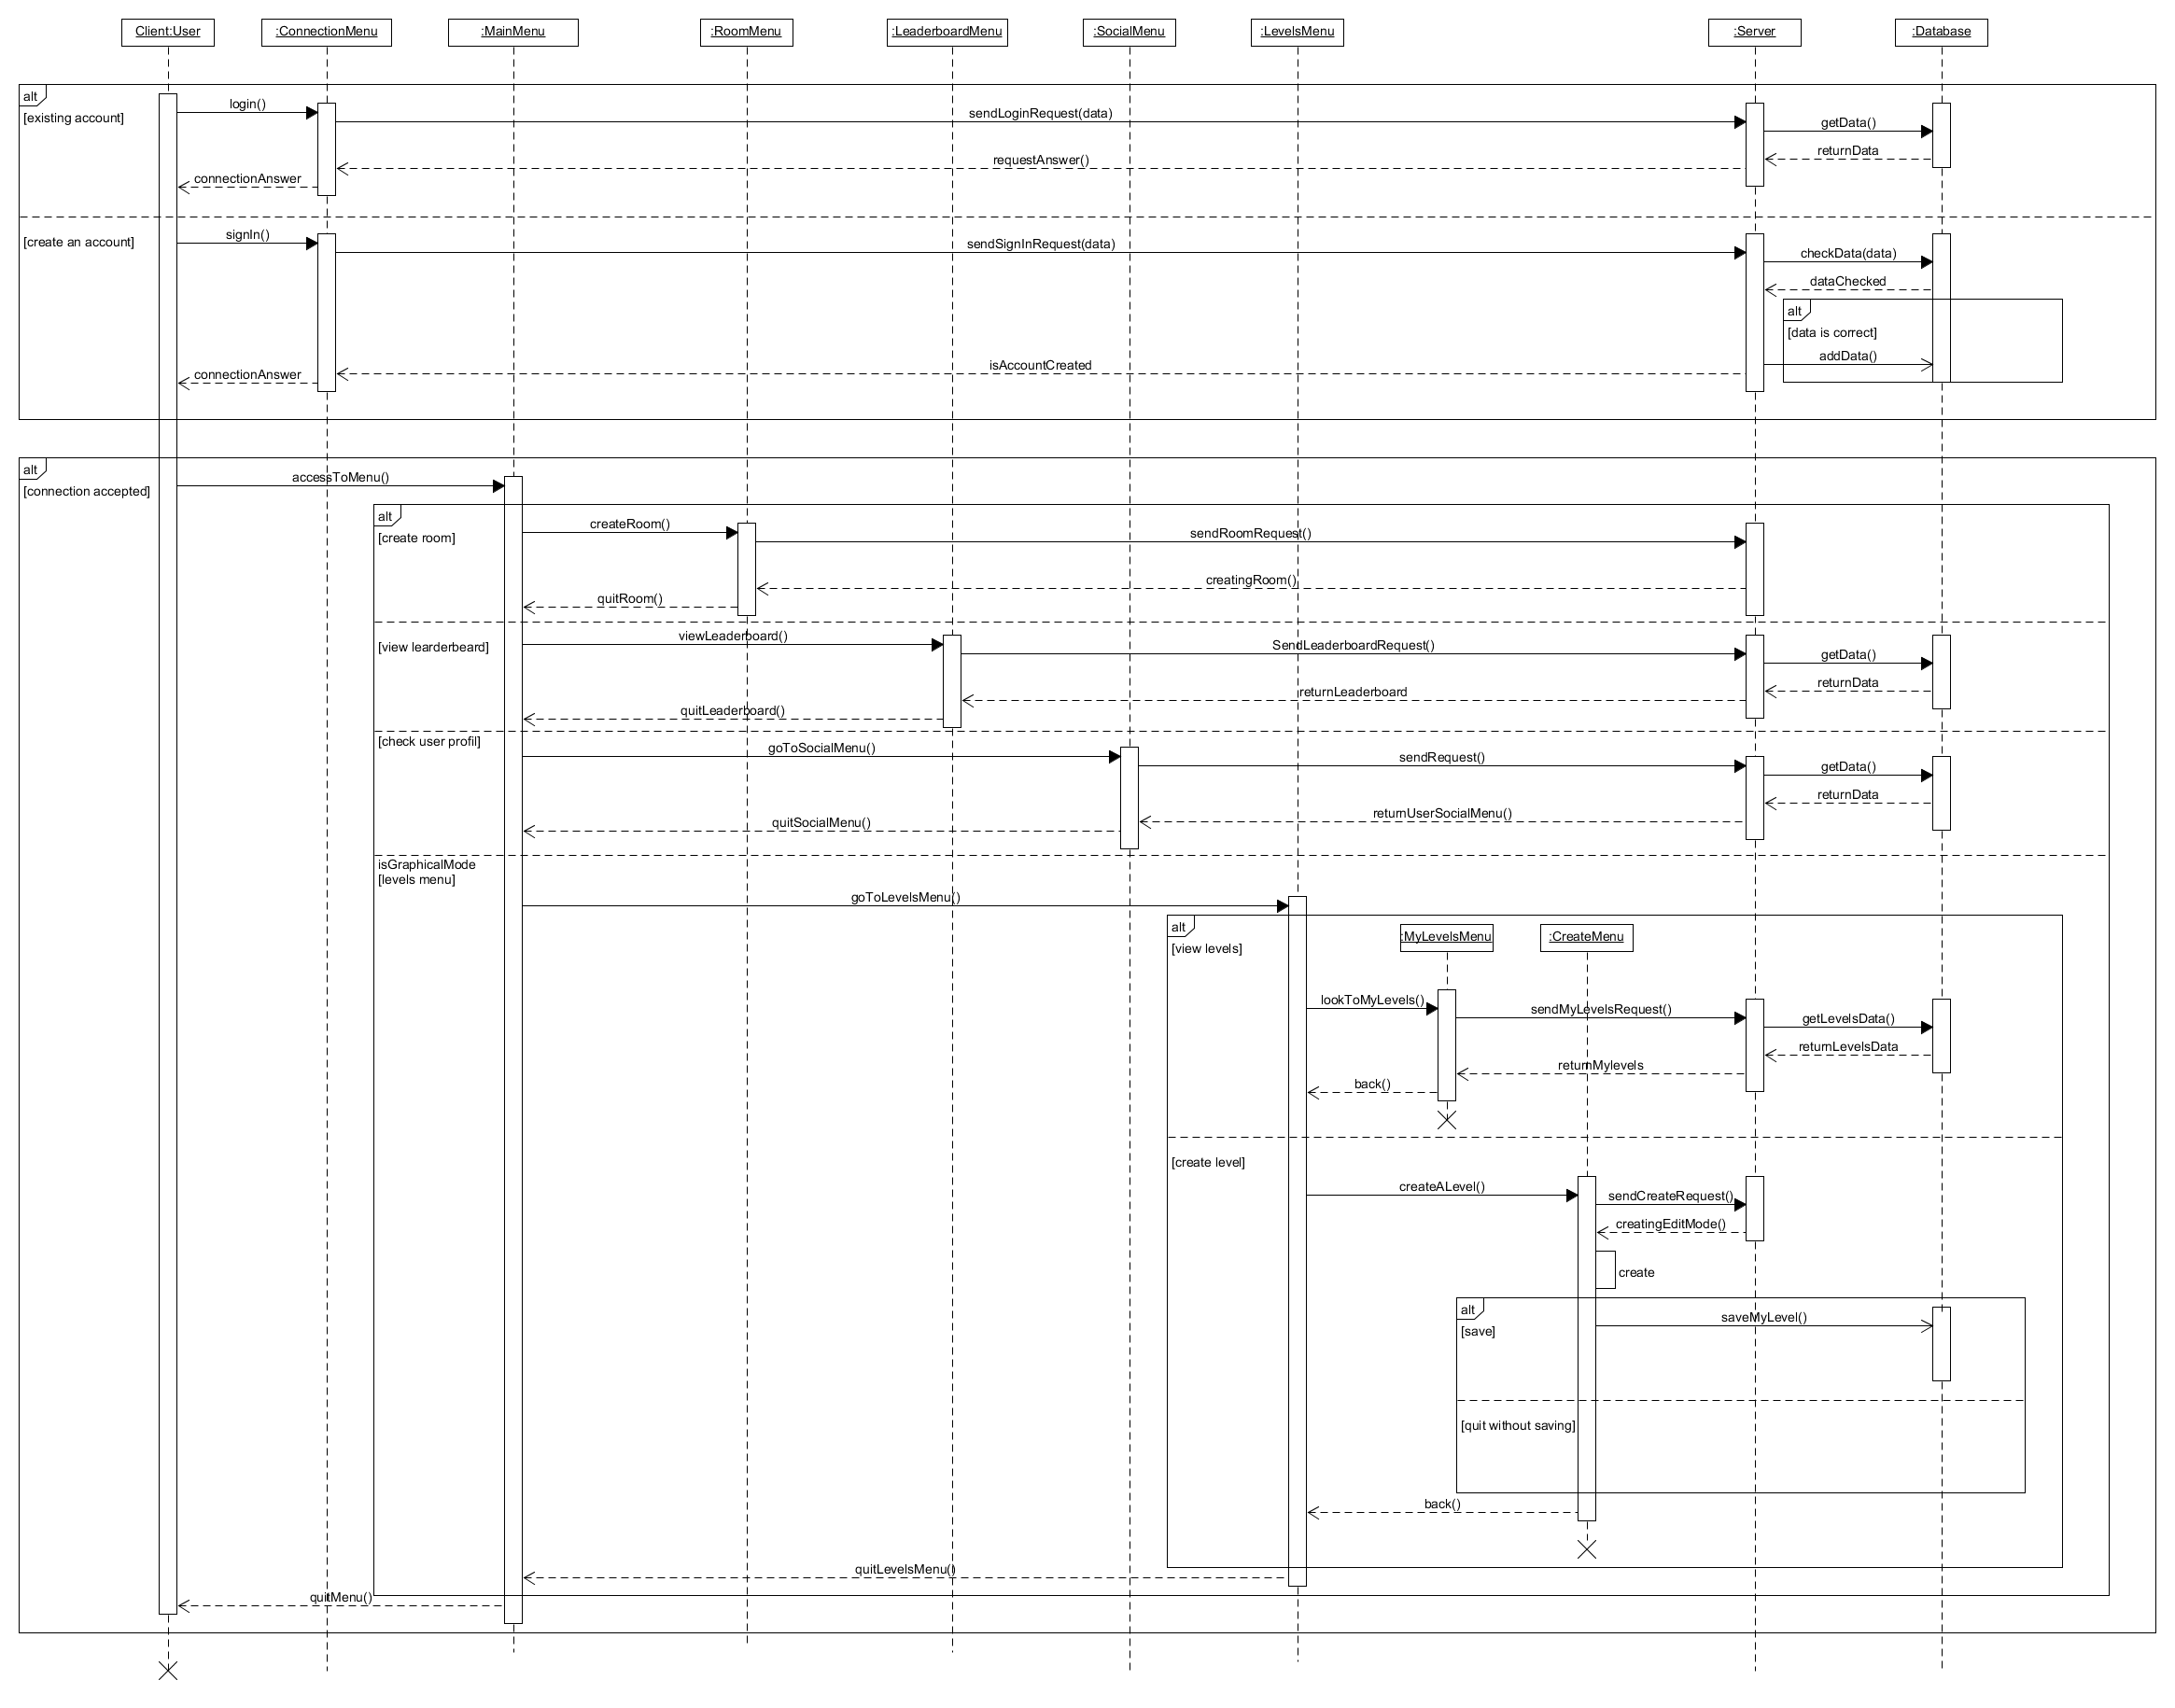
\includegraphics[scale=0.28, angle=90,origin=c]{sequence_diagram/menu_sequence.png}
    \caption{Diagramme de sequence du menu}
    \label{sequence diagram:main menu}
\end{figure}

\begin{figure}[!htbp] % TODO: note -> SMD TKS
    \centering
    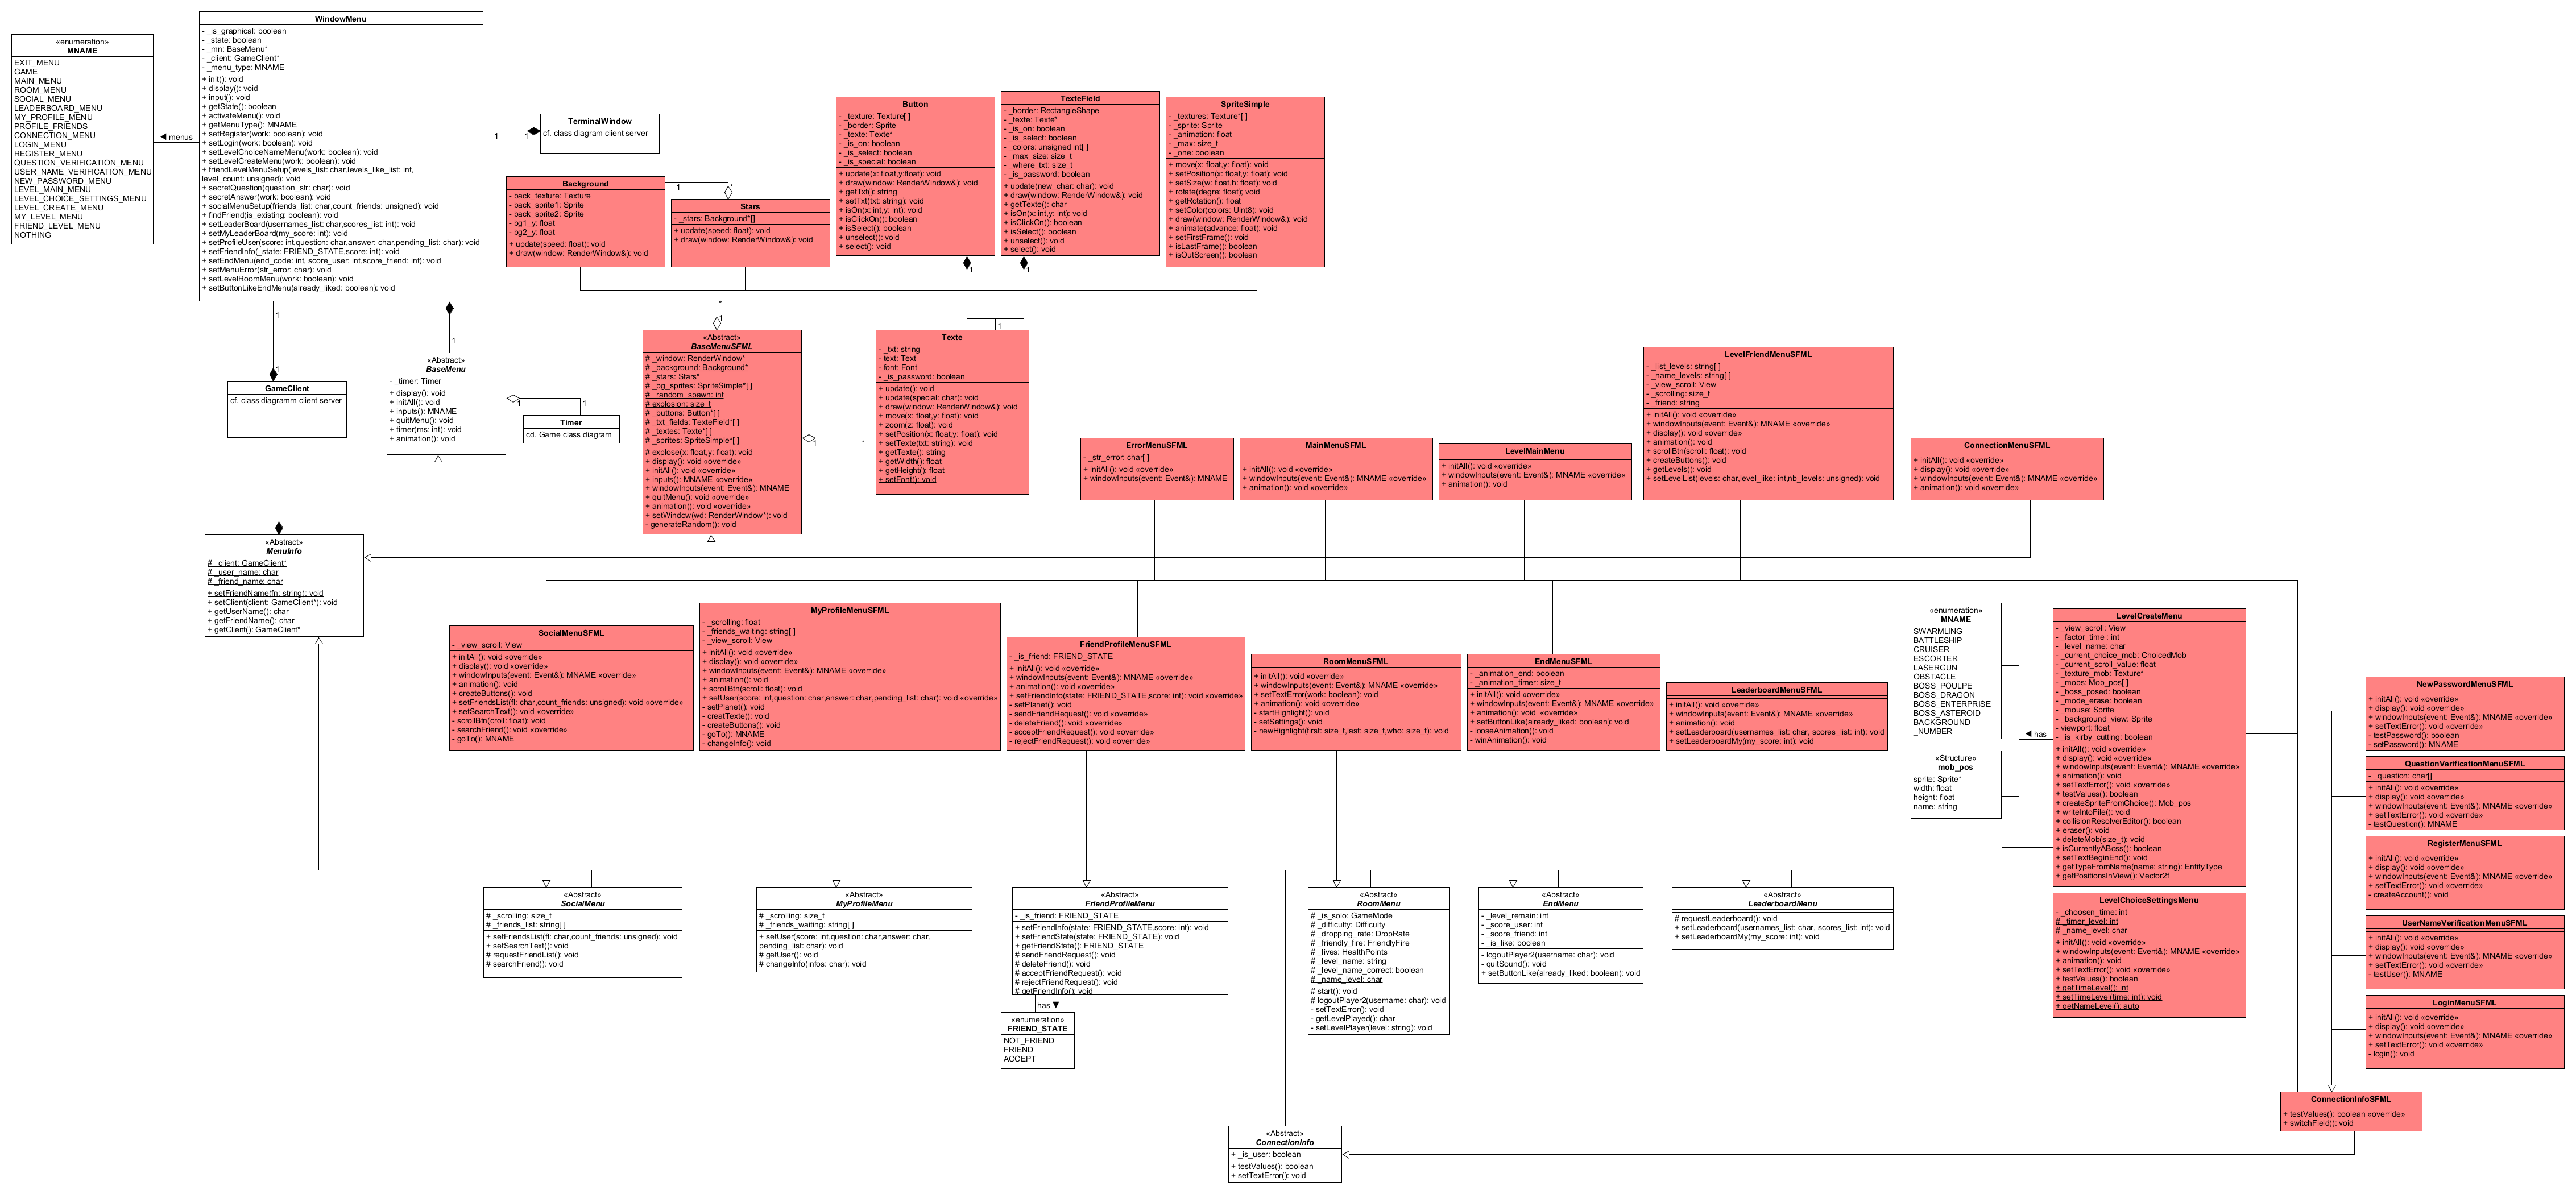
\includegraphics[scale=0.15, angle=90,origin=c]{class_diagram/class_diagram_menu_SFML.png}
    \caption{Diagramme de classe du menu - partie graphique(SFML)}
    \label{class diagram:main menu}
\end{figure}

\begin{figure}[!htbp] % TODO: note -> SMD TKS
    \centering
    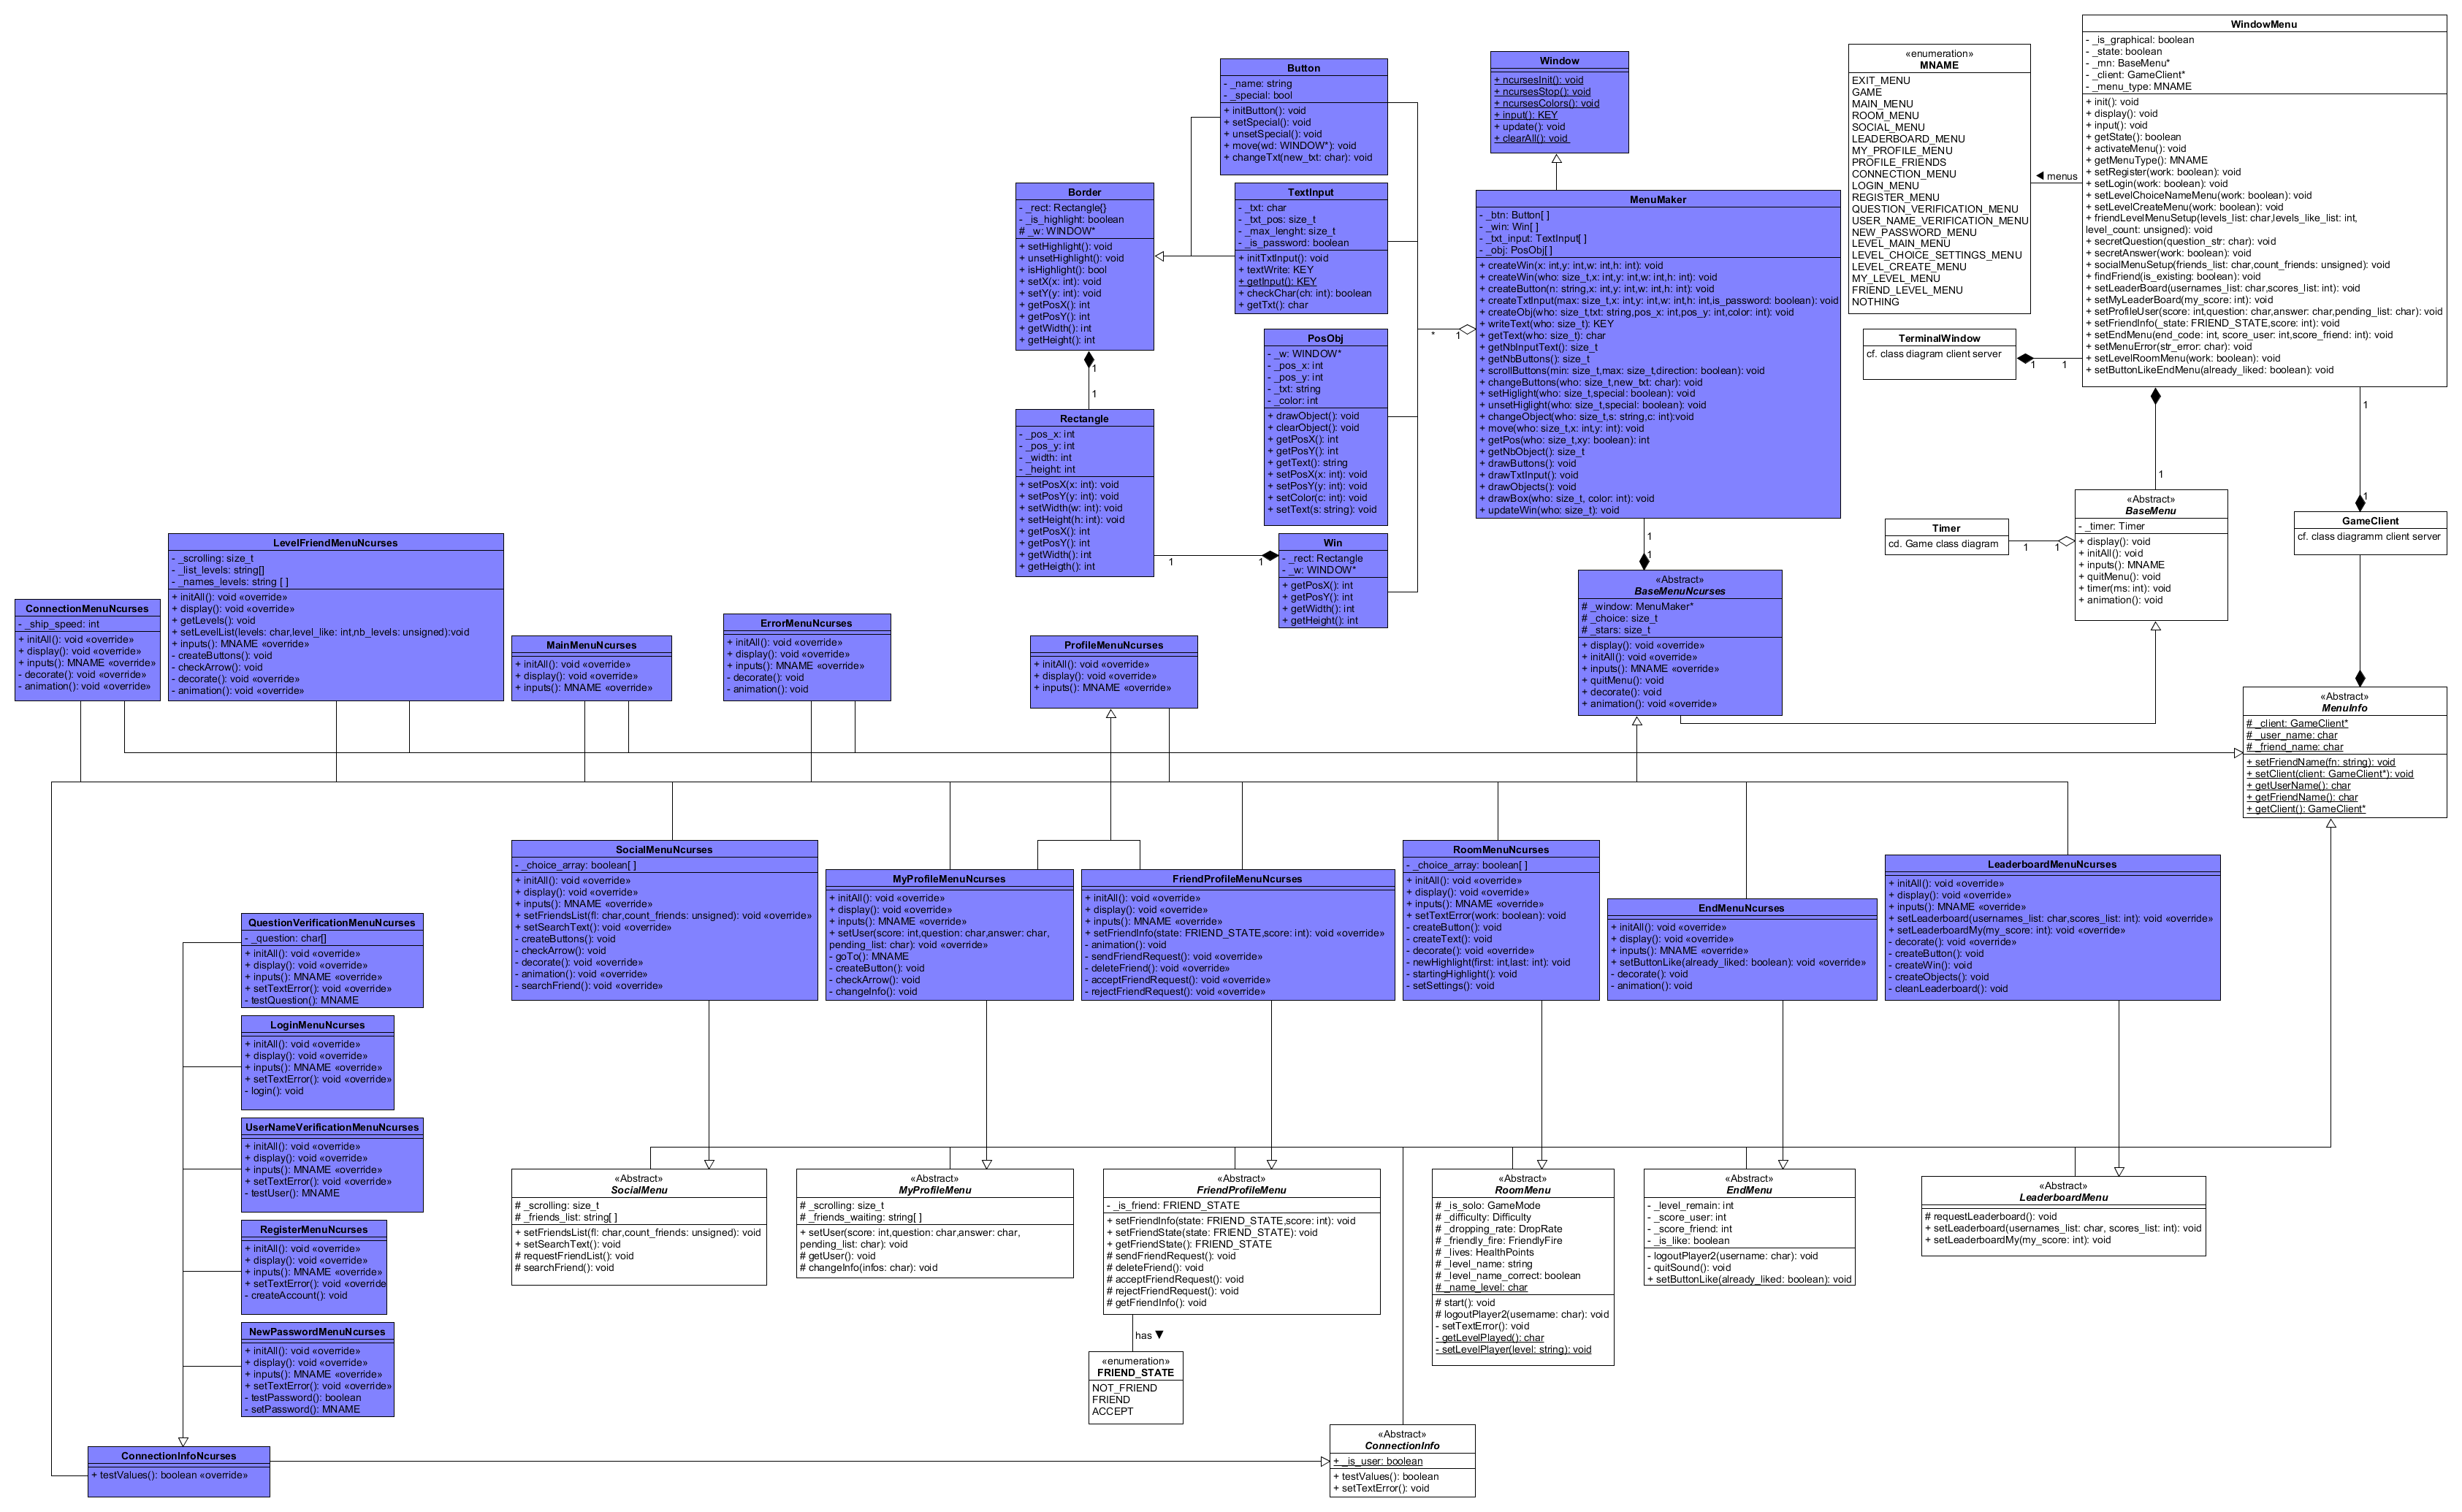
\includegraphics[scale=0.19, angle=90,origin=c]{class_diagram/class_diagram_menu_Ncurses.png}
    \caption{Diagramme de classe du menu - partie terminal(Ncurses)}
    \label{class diagram:main menu}
\end{figure}

\begin{figure}[!htbp] % TODO: note -> SMD TKS
    \centering
    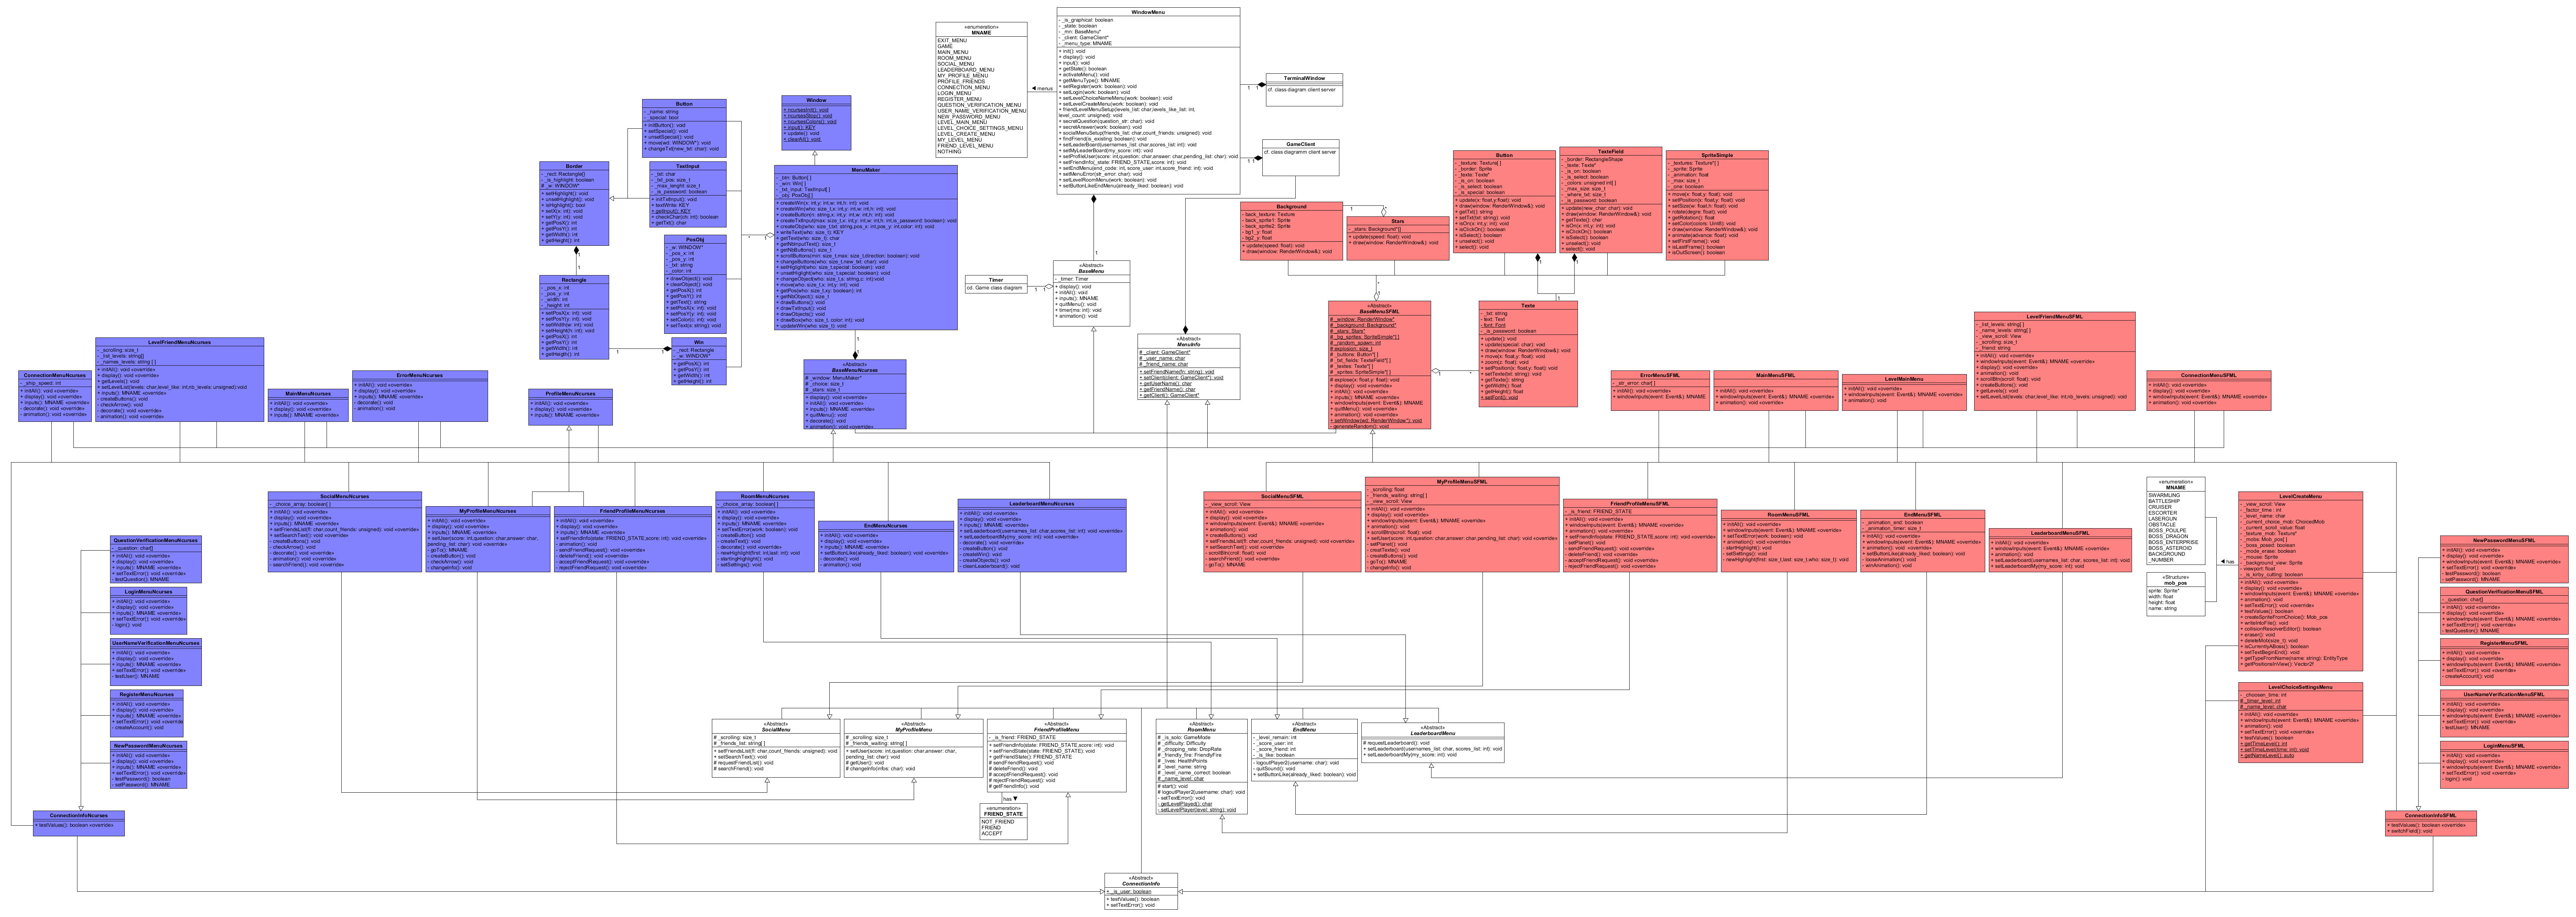
\includegraphics[scale=0.09, angle=90,origin=c]{class_diagram/class_diagram_menu.png}
    \caption{Diagramme de classe du menu- vue d'ensemble}
    \label{class diagram:main menu}
\end{figure}
\restoregeometry
\begin{flushleft}
\subsection{Online Menu}
\end{flushleft}
\begin{figure}[!htbp]
    \centering
    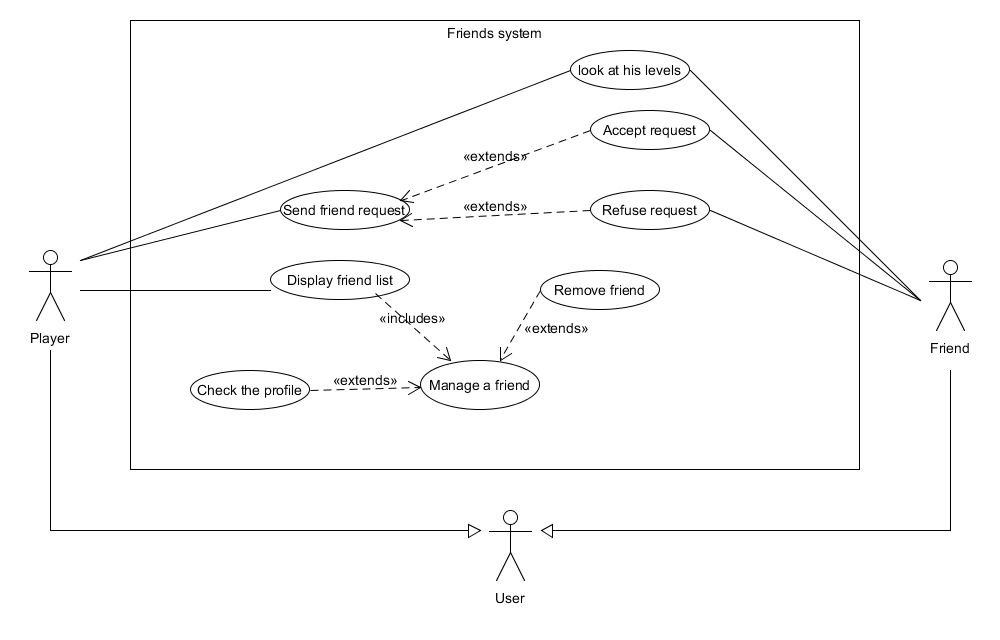
\includegraphics[scale=0.5]{use_case/Friends_System_use_case.png}
    \caption{Diagramme Use Case du côté social}
    \label{use case:online menu}
\end{figure}

\newpage
\begin{longtable}{|p{0.17\textwidth}|p{0.17\textwidth}|p{0.17\textwidth}|p{0.17\textwidth}|p{0.17\textwidth}|}
  \toprule
  \rowcolor{lightgray}
  \textbf{Use Case} & \textbf{Pré-conditions} & \textbf{Post-conditions}& \textbf{Cas général} & \textbf{Cas exceptionnels}\\
  \midrule
  Display friendlist & Avoir au moins un ami & Néant & Affiche les amis du joueur & Néant\\
  \hline
  Manage a friend & Choisir un amincissement & Néant & Remove friend &  Néant\\
  \hline
  Remove Friend & Être ami avec le joueur & Ne plus avoir le joueur en ami & Retirer l'ami de sa liste d'ami & Néant\\
  \hline
  Send friend request & Avoir le pseudo exact du joueur & Néant & La demande d'ami est envoyée & Le pseudo n'est pas correct\\
  \hline
  Look at his levels &  Avoir le pseudo exact du joueur & voit les niveaux de l'utilisateur & affiche les niveaux d'un utilisateur & aucun niveau est présent\\
  \hline
  Accept request & Avoir reçu une demande d'ami & Avoir un nouvel ami & Les deux joueurs s'ajoutent mutuellement dans leur liste d'amis & Néant\\
  \hline
  Refuse request & Avoir reçu une demande d'amis & Néant & La demande d'ami est supprimée & Néant\\
  \hline
  Check profile & Avoir le pseudo exact & Néant & Affiche le profil du joueur au pseudo correspondant & Le pseudo n'est pas correct\\
  \bottomrule
\end{longtable}
\begin{center}
Explication Use Case de Online Menu : Menu où nous regardons notre liste d'ami(e)s et pouvons envoyer une invitation, supprimer un(e) ami(e), annuler une demande, etc. 
\end{center}
\begin{figure}[!htbp]% TODO : note -> SMD TKS
    \centering
    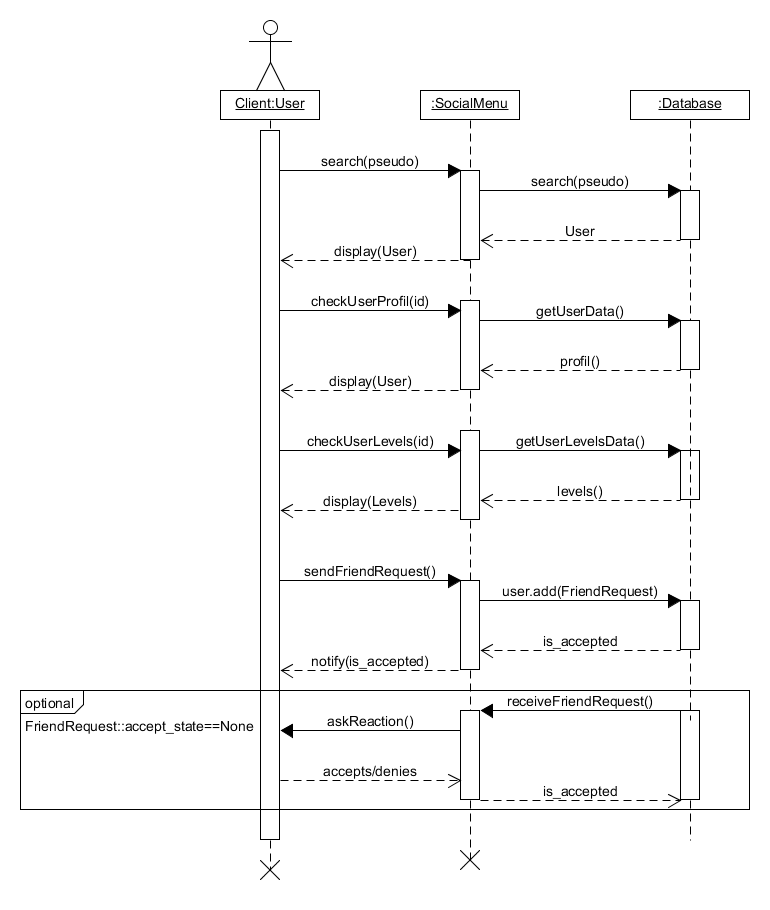
\includegraphics[scale=0.5]{sequence_diagram/uml_sequence_online.png}
    \caption{Diagramme de séquence des amis}
    \label{sequence diagram:online menu}
\end{figure}
\begin{figure}[!htbp]
    \centering
    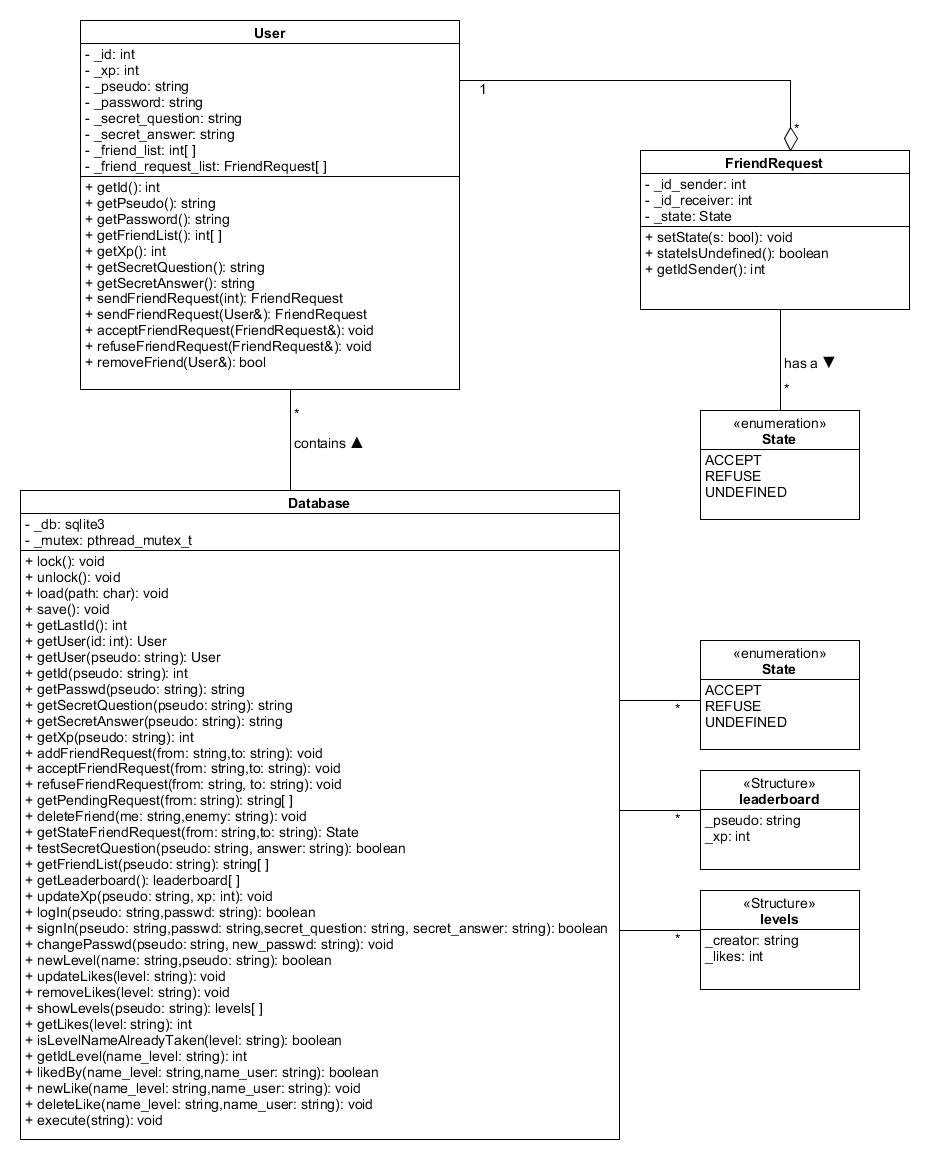
\includegraphics[scale=0.5]{class_diagram/class_diagram_database.png}
    \caption{Diagramme de classe de la database} %le légendaire
    \label{diagram class:connection menu}
\end{figure}
\newpage
\subsection{Game}
\begin{figure}[!htbp]
    \centering
    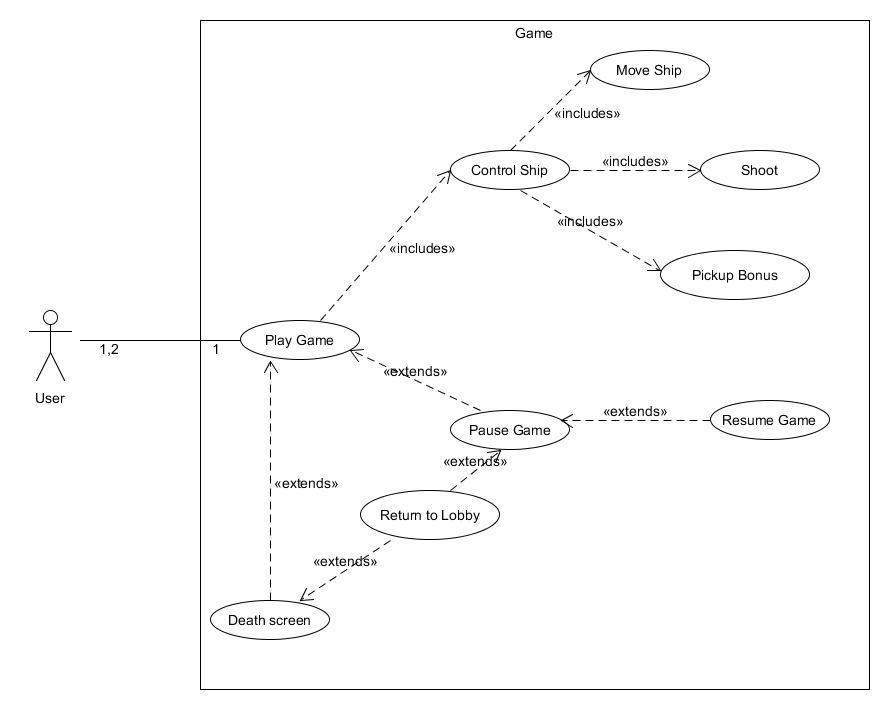
\includegraphics[scale=0.5]{use_case/use-case-game.png}
    \caption{Diagramme Use Case de la partie}
    \label{use case:game}
\end{figure}
\newpage
\begin{longtable}{|p{0.22\textwidth}|p{0.22\textwidth}|p{0.22\textwidth}|p{0.22\textwidth}|}
  \toprule
  \rowcolor{lightgray}
  \textbf{Use Case} & \textbf{Pré-conditions} & \textbf{Post-conditions}& \textbf{Cas général}\\
  \midrule
  Play Game & est connecté au jeu & néant & c'est l'écran principal pour les 1/2 joueur(s)\\
  \hline
  Pause Game & le jeu tourne & le jeu est arrêté & le jeu est mis en pause\\
  \hline
  Resume Game & le jeu est arrêté & le jeu tourne & le jeu est remis en route\\
  \hline
  Return to Lobby & le jeu est arrêté & le joueur est dans le lobby & termine la partie et retourne dans le lobby\\
  
  \hline
  Control Ship & le jeu tourne & néant & tout ce qui peut être fait avec le vaisseau\\
  \hline
  Move Ship & le jeu tourne & le vaisseau bouge & le vaisseau peut bouger dans les directions sans sortir de l'écran\\
  \hline
  Shoot & le jeu tourne & néant & tire des projectiles qui endommagent à la collision\\
  \hline
  Pickup Power Ups & le jeu tourne & le vaisseau a un bonus & bouger le vaisseau vers le power up pour utiliser l'arme\\
  \hline
  Death Screen & le joueur a perdu & quitter vers le lobby & le menu qui apparait quand le joueur perd\\
  \hline
  End Credits & gagner & retour au menu principal & les crédits sont montrés à la fin du jeu\\
  \hline
  Like & joue un niveau créé & le niveau a un like en plus & ajoute un like au niveau\\
  \bottomrule
\end{longtable}
\begin{center}
Explication Use Case de Game : Le déroulement du jeu ainsi que ses possibilités.
\end{center}
\newgeometry{vmargin=2cm}
\begin{figure}[!htbp]
    \centering
    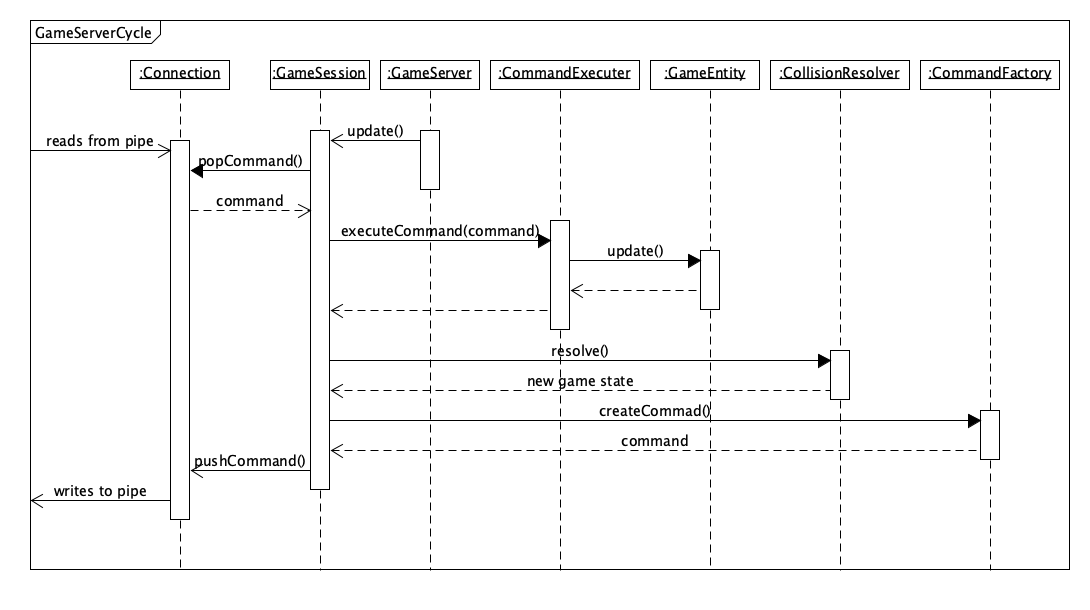
\includegraphics[scale=0.6, angle=90]{sequence_diagram/game_server_sequence.png}
    \caption{diagramme de séquence serveur de jeu}
    \label{sequence diagram:game server}
\end{figure}

\begin{figure}[!htbp]
    \centering
    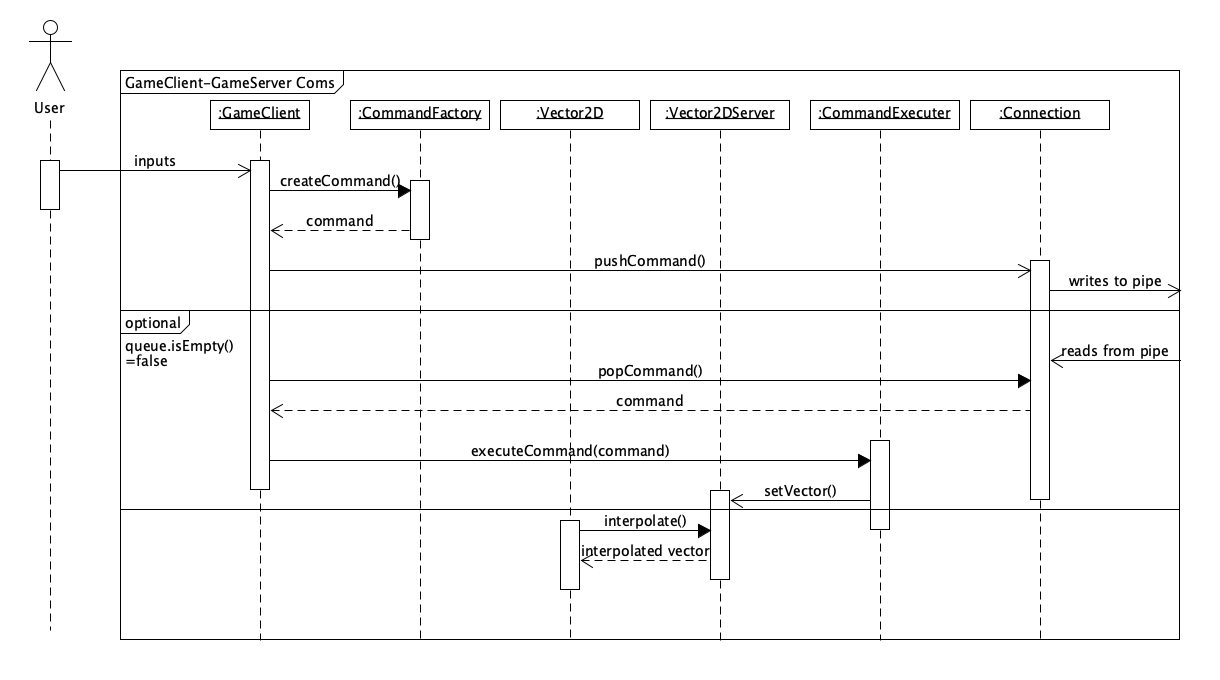
\includegraphics[scale=0.55, angle=90]{sequence_diagram/game_client_server_sequence.png}
    \caption{diagramme de séquence client serveur de jeu}
    \label{sequence diagram:game client server}
\end{figure}
\restoregeometry

\begin{figure}[!htbp]% TODO = note -> SMD TKS
    \centering
    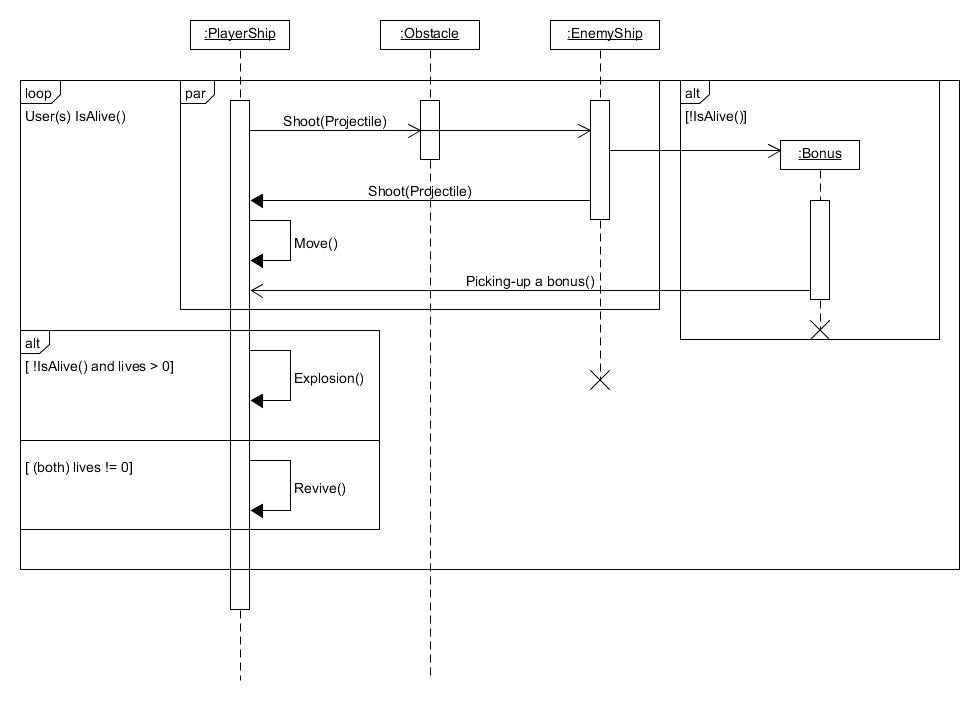
\includegraphics[scale=0.5]{sequence_diagram/game_sequence.jpg}
    \caption{diagramme de séquence de la partie}
    \label{sequence diagram:game}
\end{figure}

\newgeometry{vmargin=2cm}
\label{class diagram:game}
\begin{figure}[!htbp]
    \centering
    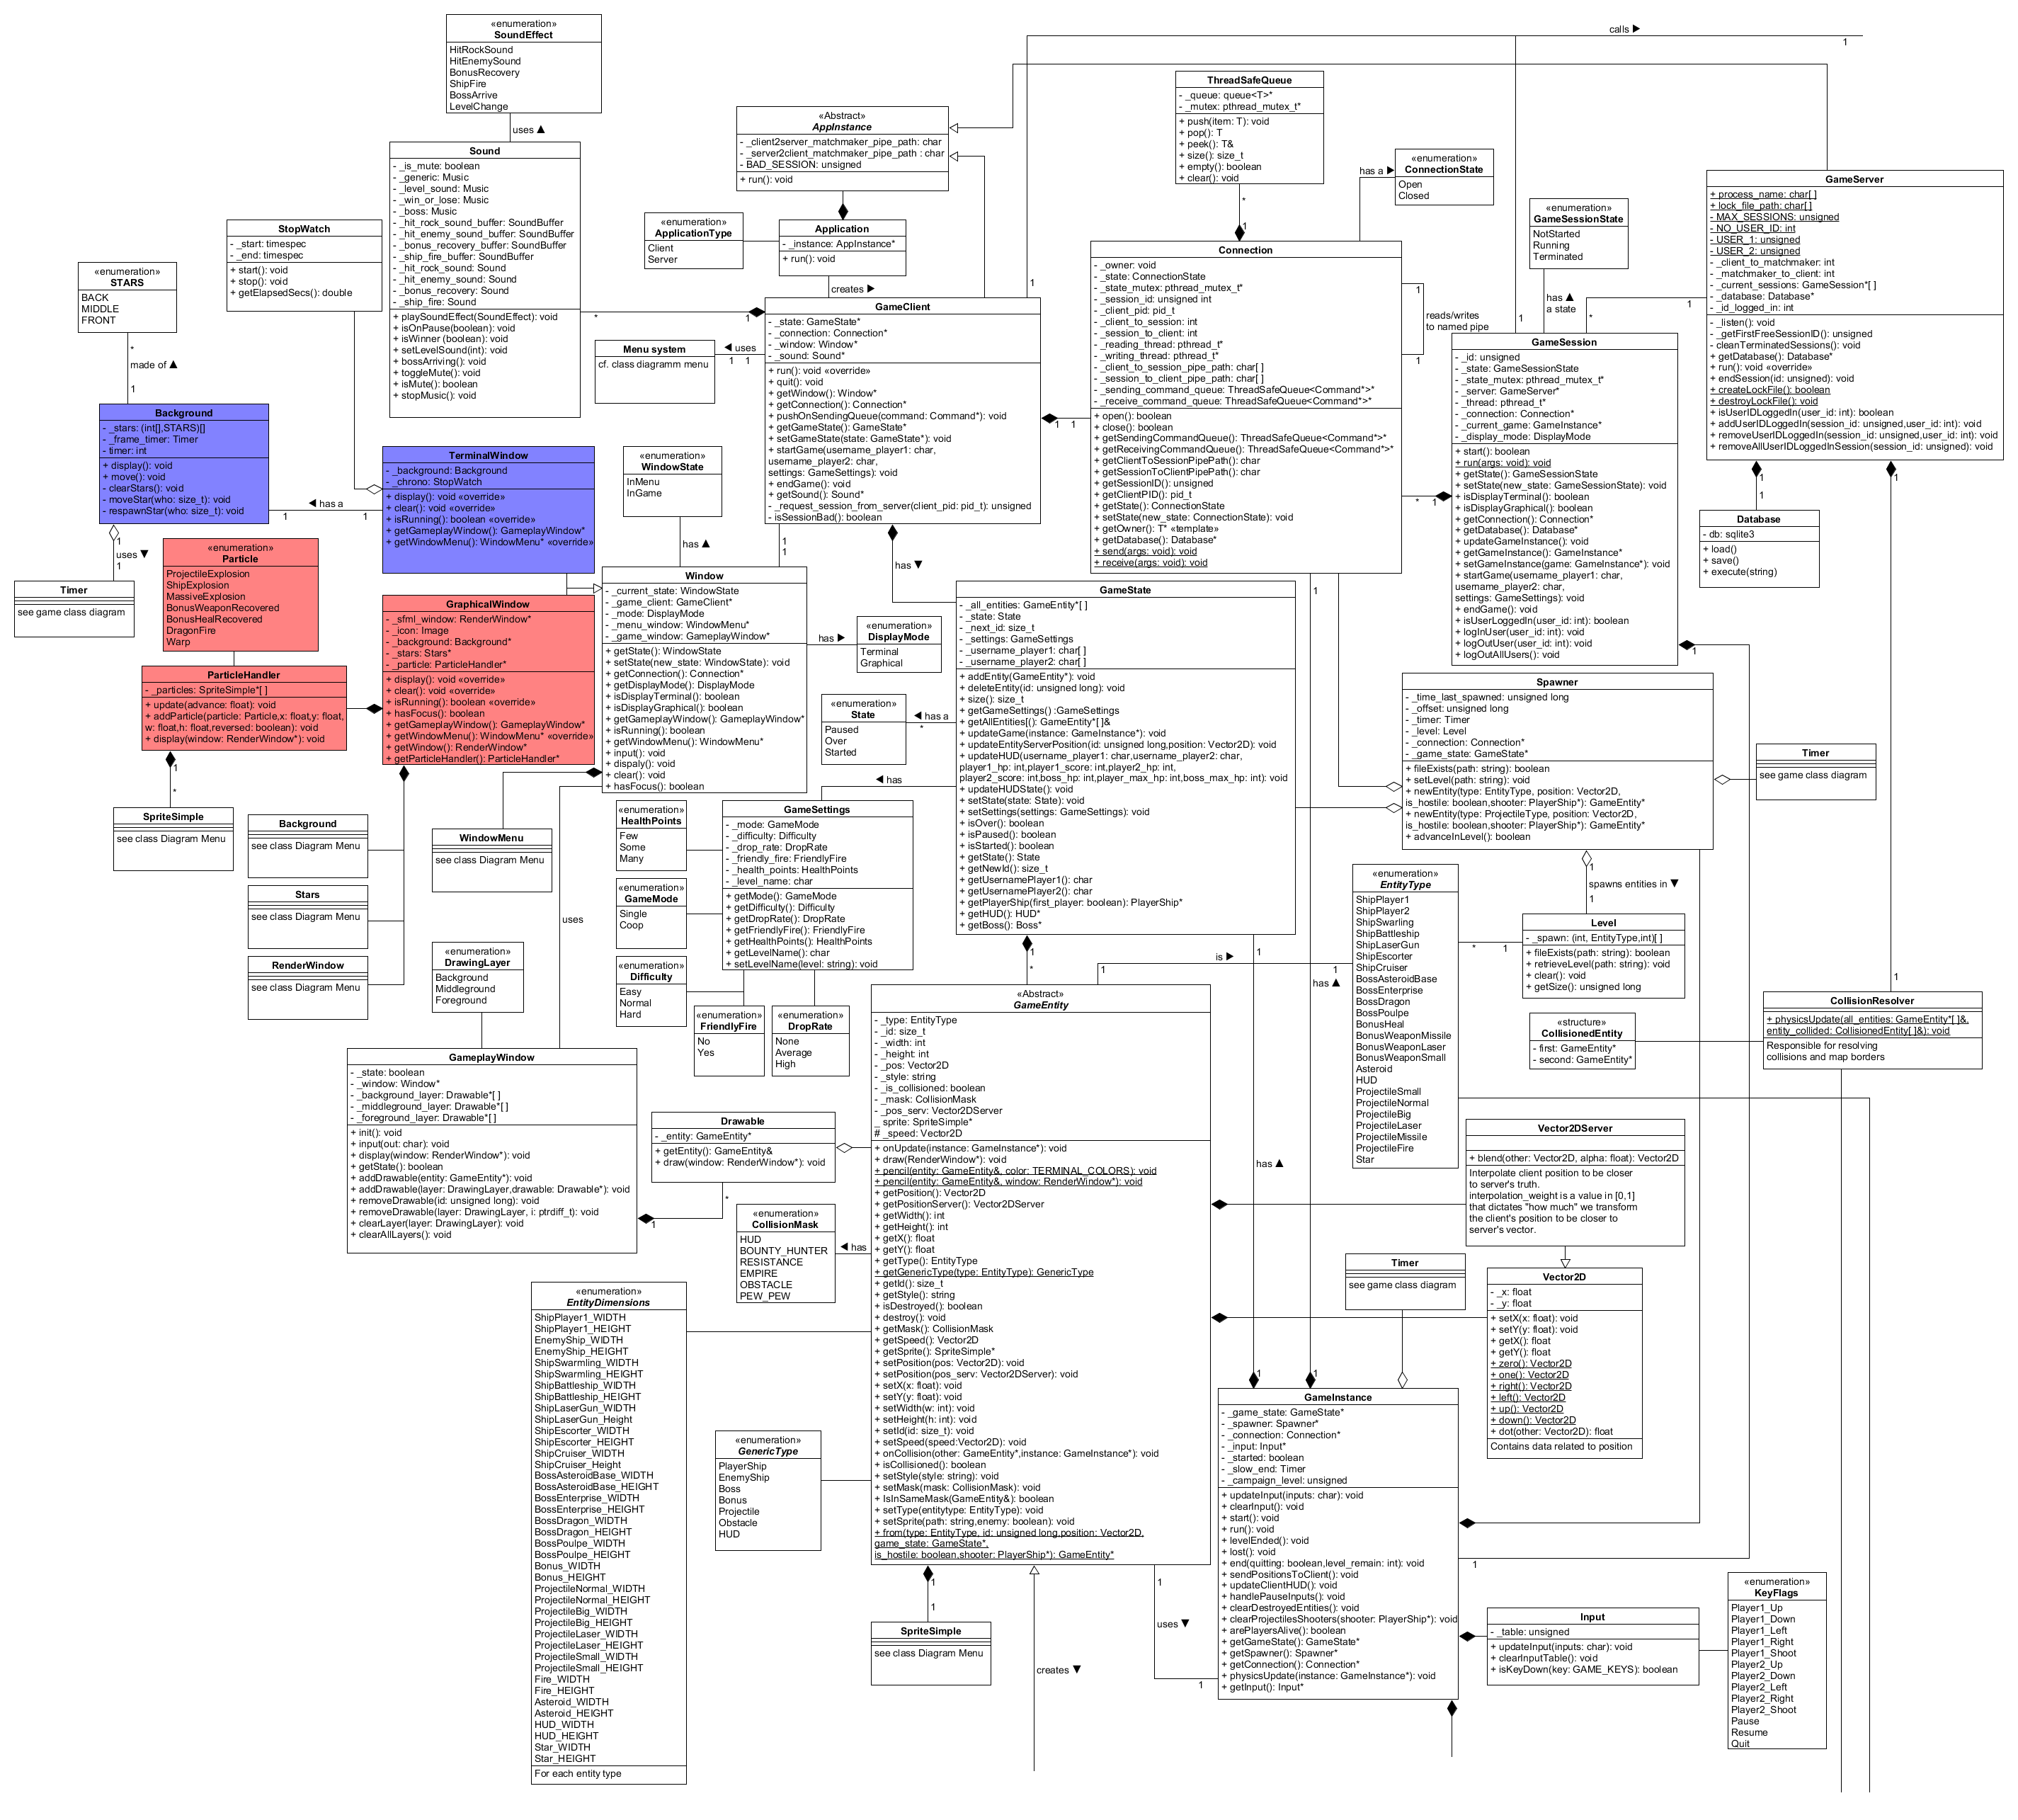
\includegraphics[scale=0.20, angle=90]{class_diagram/class_diagramm_client_server.png}
    \caption{Diagramme de classe du jeu(1)- partie sur le serveur et une partie du client}
    \label{class diagram:game-server}
\end{figure}

\begin{figure}[!htbp]
    \centering
    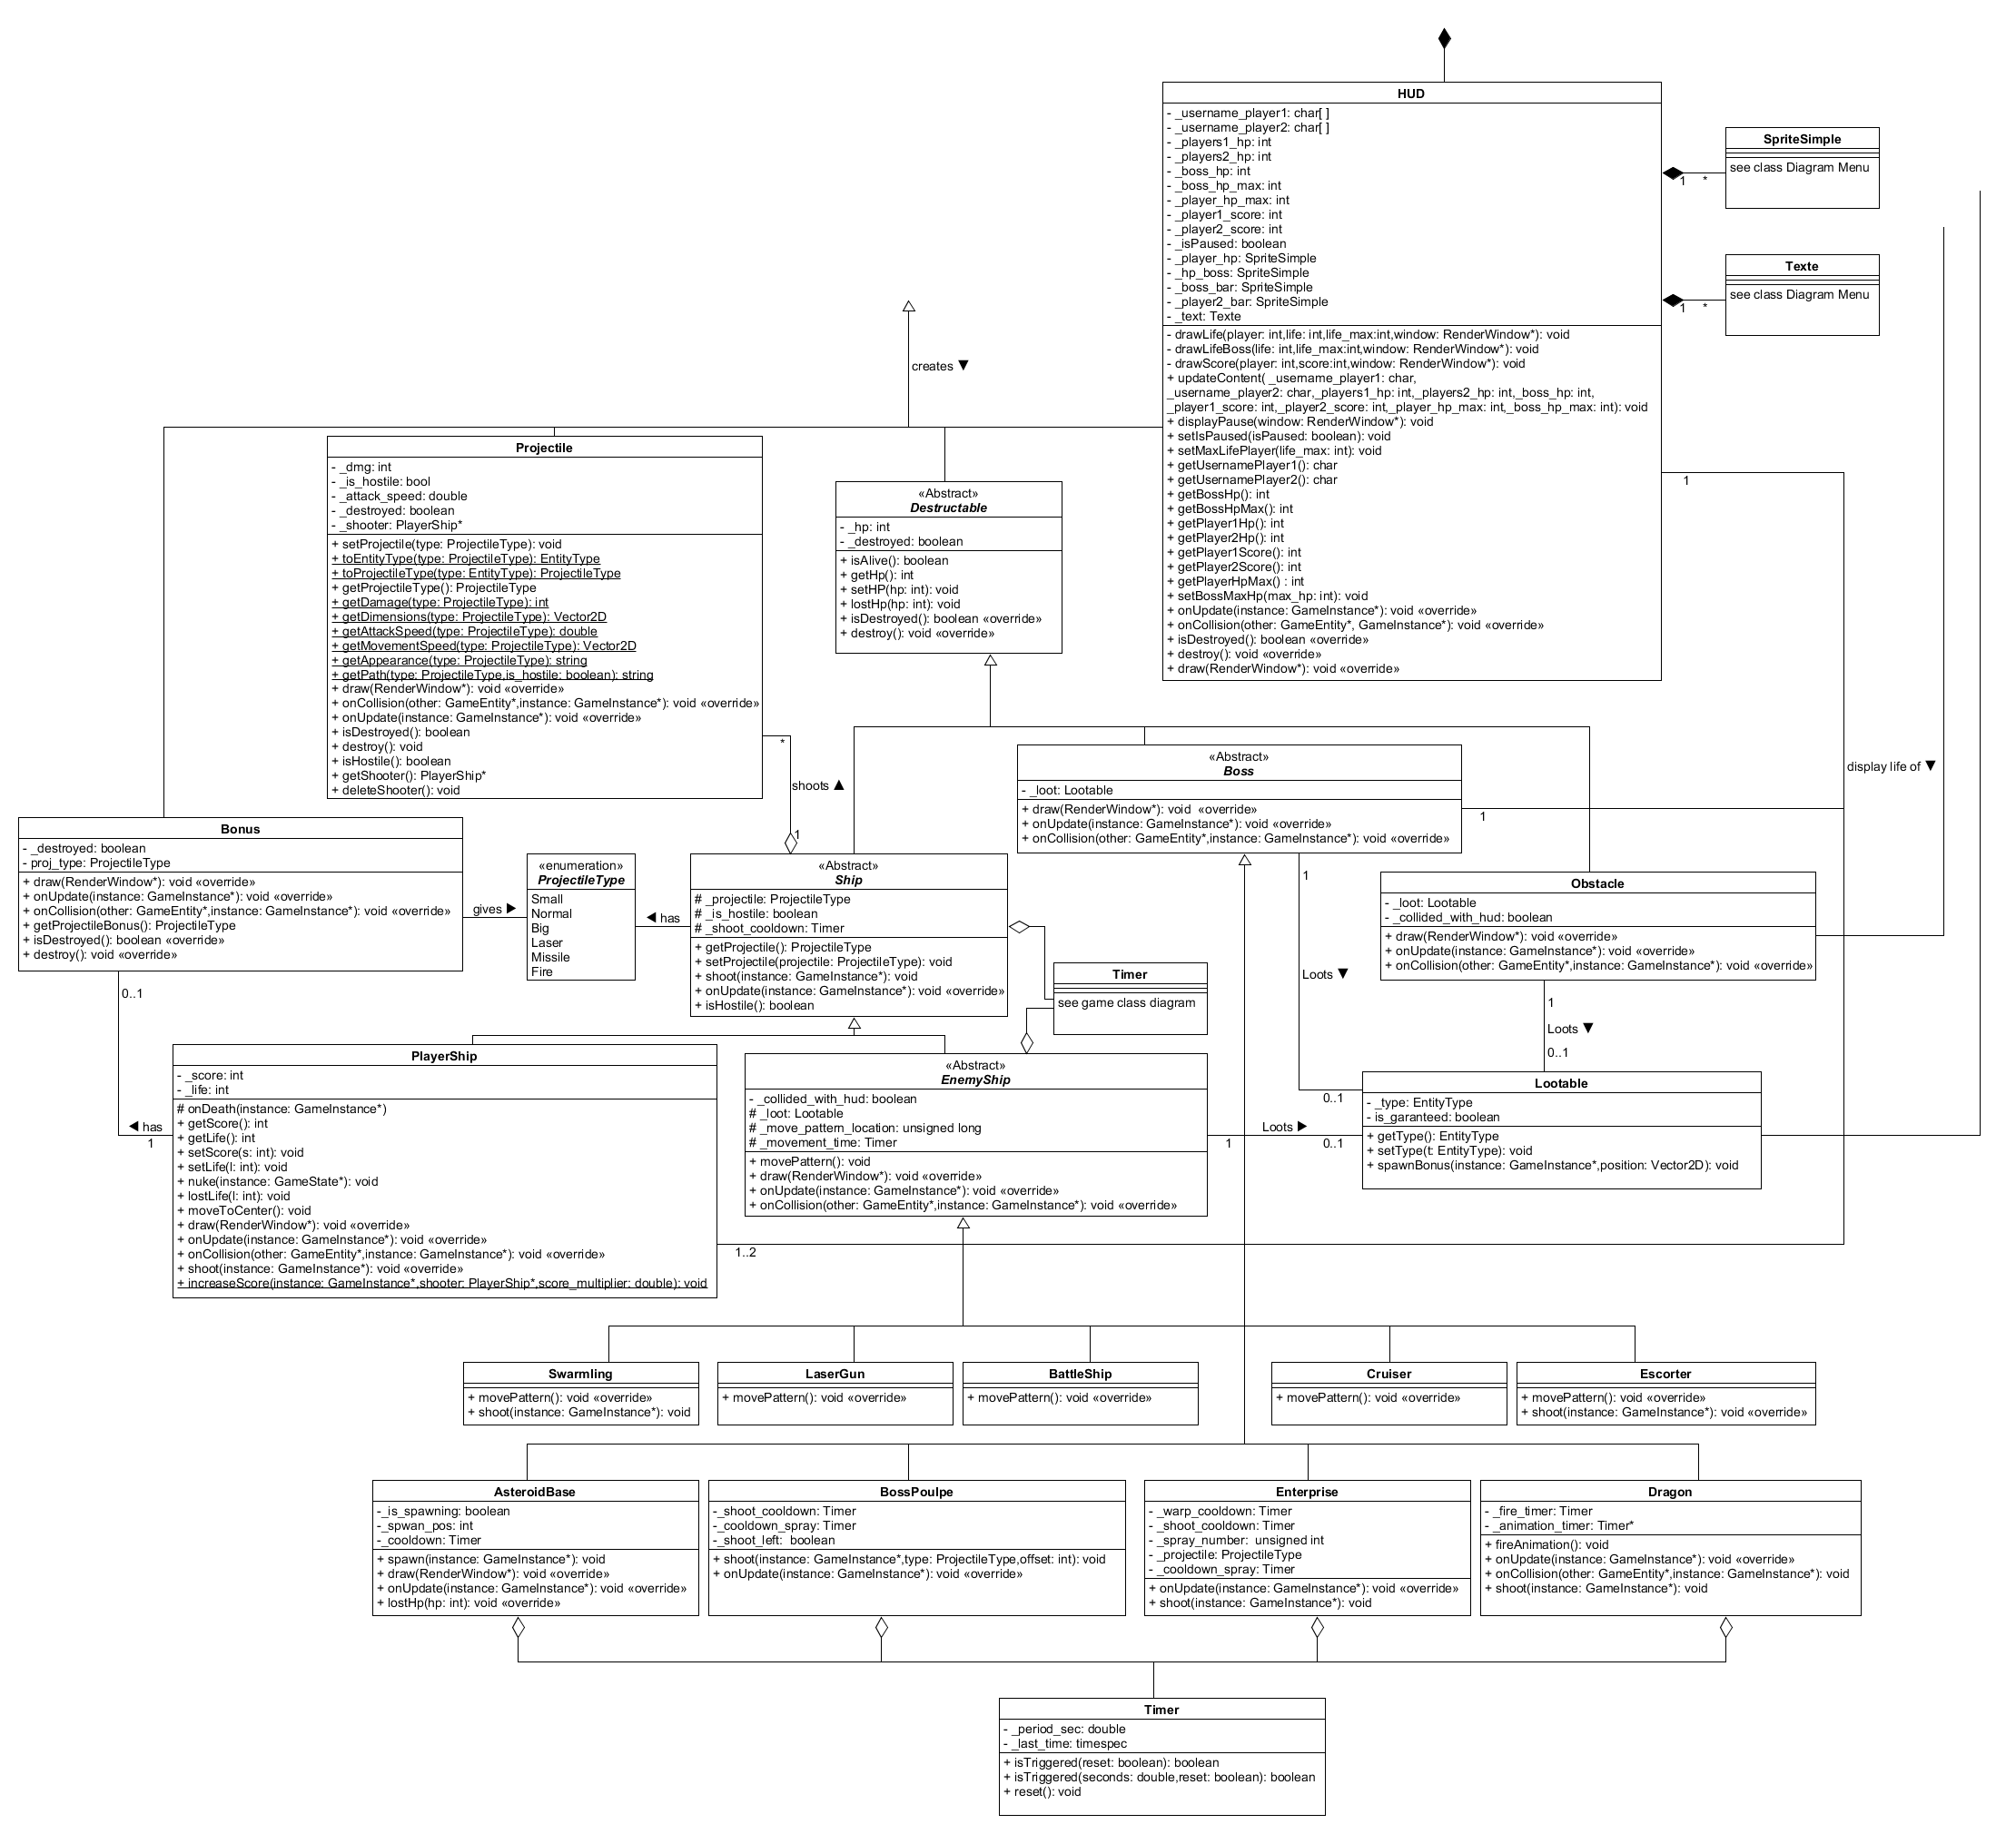
\includegraphics[scale=0.25, angle=90]{class_diagram/class_diagramm_game_logic.png}
    \caption{Diagramme de classe du jeu(2)- partie sur la logique du jeu}
    \label{class diagram:game-gameplay}
\end{figure}

\begin{figure}[!htbp]
    \centering
    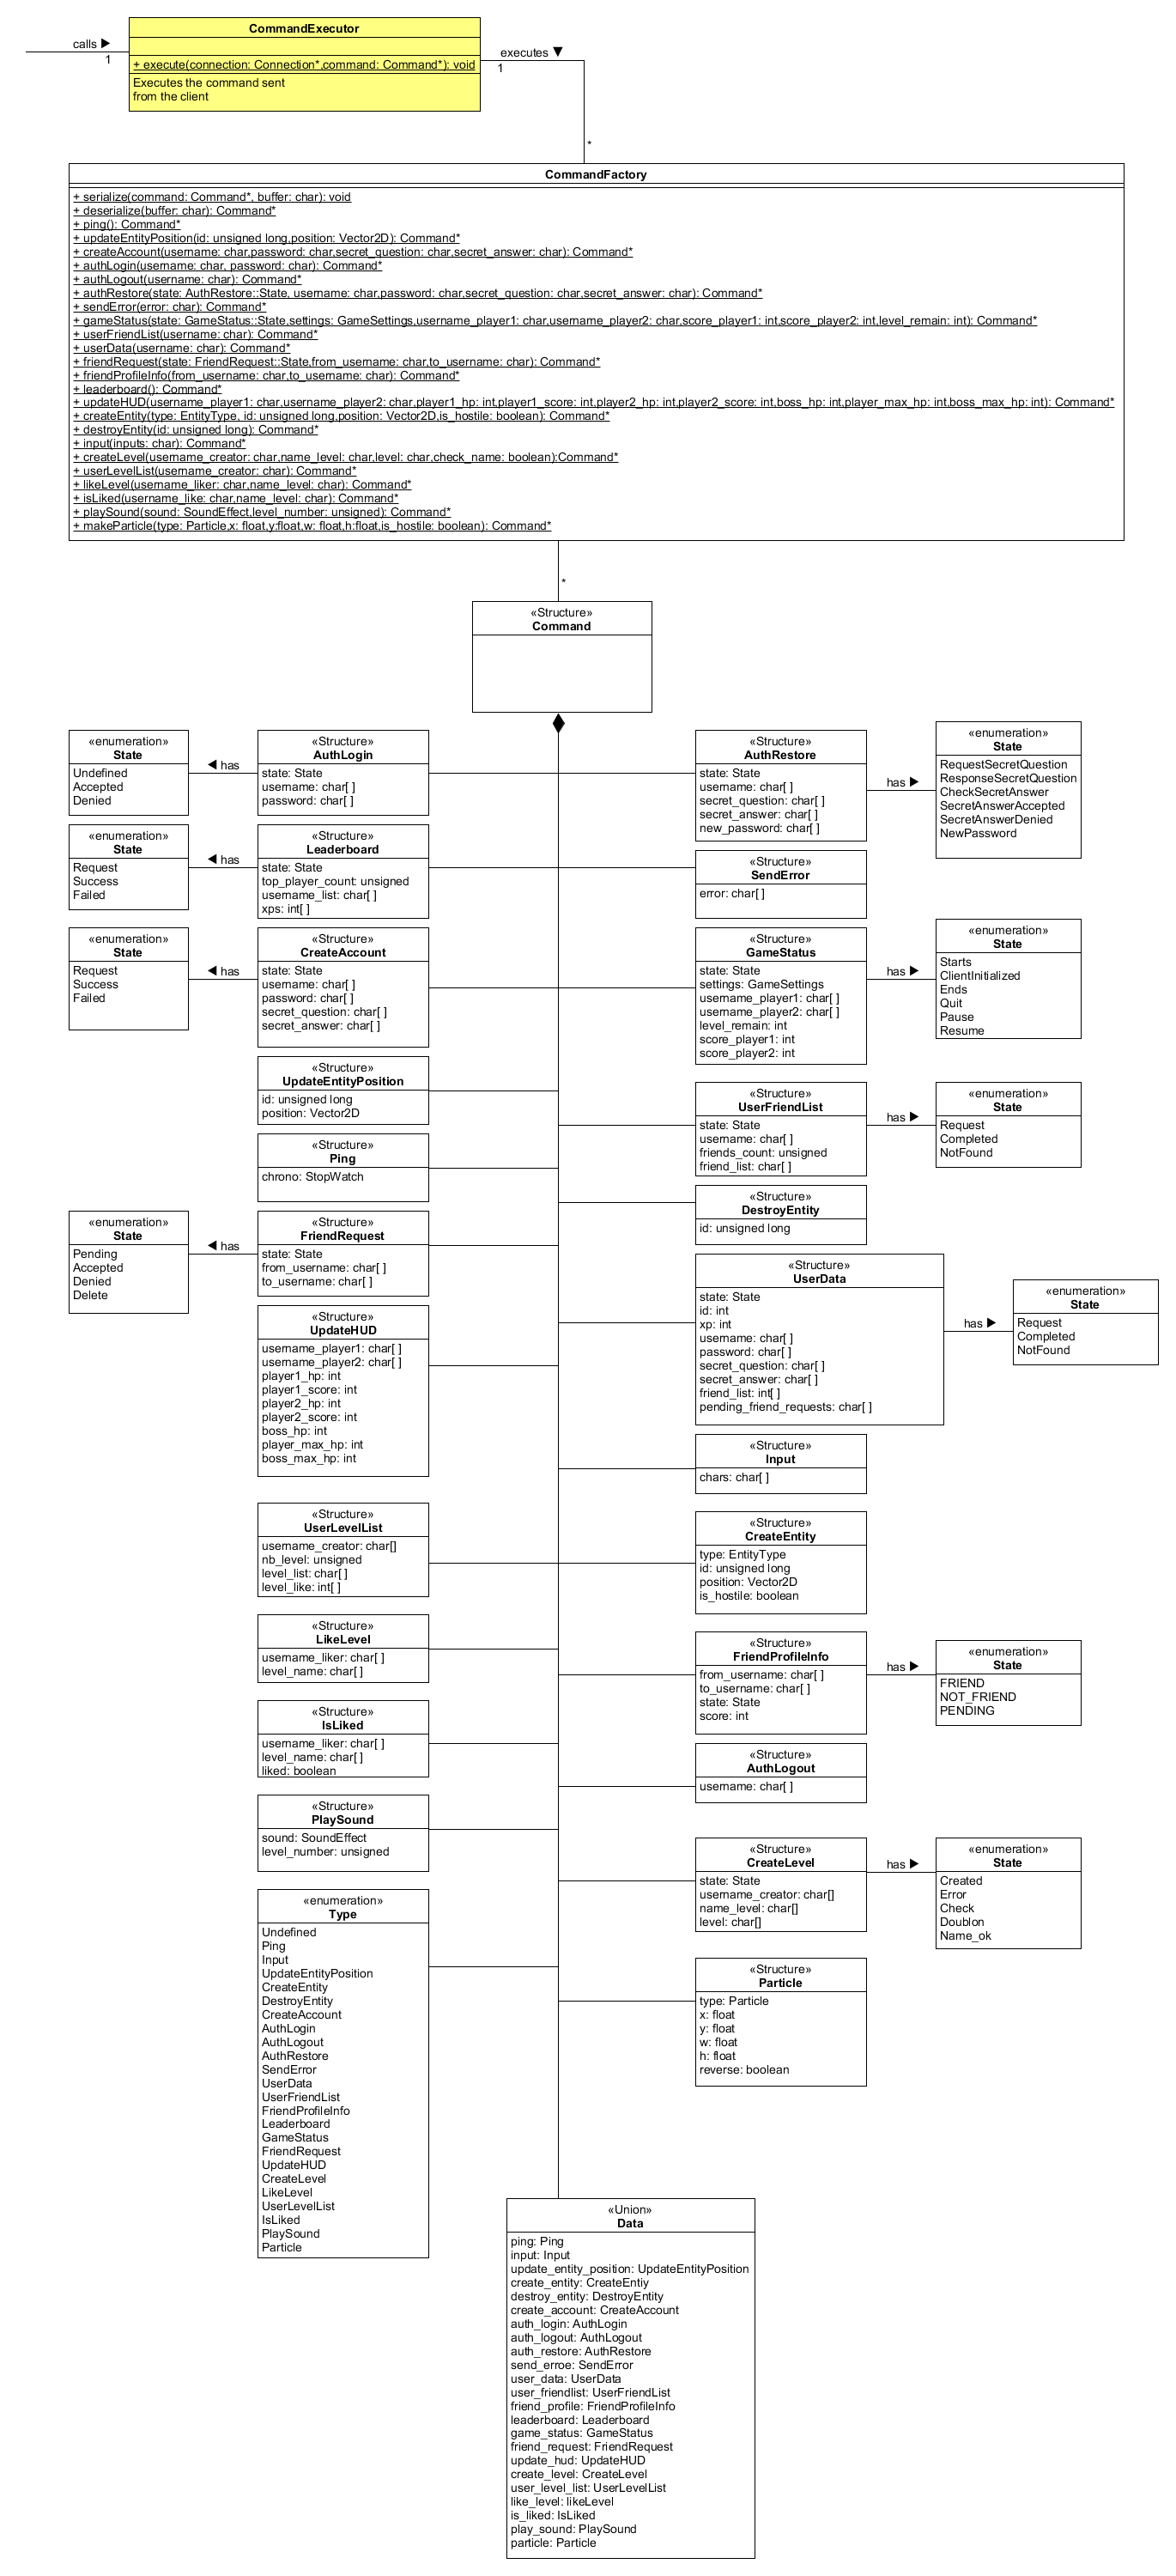
\includegraphics[scale=0.21, angle=0]{class_diagram/class_diagramm_command.png}
    \caption{Diagramme de classe du jeu(3) - partie sur les commandes}
    \label{class diagram:game-gameplay}
\end{figure}
\section{Explications pour le diagramme de la partie sur les commandes.}
La structure Command représente une commande, elle peut être lu et écrite depuis un pipe.L'union quant à elle est la liste de toutes les commandes possibles(une structure par type de commande).L'énumération "Type" représente tous les types de commandes afin de faciliter la sérialisation. Les différentes commandes sont:
\newline
\begin{itemize}
    \item Ping: Fais un aller-retour jusqu'au serveur et affiche le temps que cela a mis.Cela sert surtout à debugger et à montrer que le client se connecte au serveur.
    \item Input: Envoies une liste des touches appuyées dans une frame par le client.La session les récupère et réalise les actions demandées.
    \item UpdateEntityPosition: Le serveur envoie cette commande au client une fois que les collisions sont résolues afin de mettre à jour le vecteur de position présent sur le serveur.
    \item CreateEntity: Le serveur envoie cette commande au client quand il crée une nouvelle entité.
    \item DestroyEntity: Le serveur envoie cette commande au client quand il détruit une entité.
    \item CreateAccount: Commande envoyée par le client au serveur("Request").Le serveur crée potentiellement le compte dans la base de données("Success","Failed") et renvoie l'information au client.
    \item AuthLogin: Le client envoie cette commande au serveur.Le serveur renvoie une réponse qui peut avoir plusieurs états "undefined","Accepted","Denied" qui sont respectivement l'état de base que le client envoie au serveur, l'état signifiant que le login est une réussit et l'état de l'échec du login.
    \item AuthLogout: Commande envoyée par le client au serveur pour déconnecter un utilisateur, principalement utilisé pour déconnecter le second joueur étant donné que le premier utilisateur ne peut pas se déconnecter du jeu sans le quitter.
    \item AuthRestore: Commande utilisée lorsqu'un utilisateur a oublié son mot de passe.Il fera plusieurs allers-retours entre le client et le serveur et aura plusieurs états pendant l'exécution comme AuthLogin.
    \item SendError: Envoie une erreur à l'utilisateur.
    \item UserData: Le client l'envoie afin de recevoir les informations de l'utilisateur.Elle a aussi plusieurs états en cours de route.
    \item UserFriendList: Une commande envoyée par le client afin d'avoir les informations concernant la liste d'amis de l'utilisateur.
    \item FriendPofileInfo: Commande afin de récupérer les informations sur le profile d'un ami.
    \item Leaderboard: Commande qui demande les informations du leaderboard du serveur.
    \item GameStatus: Préviens la session/le client qu'une partie a commencé ou s'est terminée.
    \item FriendRequest: Le client envoie cette commmande au serveur pour le notifier qu'un utilisateur a envoyé une demande d'ami à un autre utilisateur.
    \item UpdateHUD: Commande envoyée par le serveur au client afin de mettre à jour l'HUD.
    \item CreateLevel: Une commande que le client peut utiliser pour faire 2 choses: savoir si un nom est déjà utilisé pour un niveau et pour créer un niveau.
    \item UserLevelList: Renvoie au client tous les niveaux créés par l'utilisateur(username\_creator).
    \item LikeLevel: Like un niveau.
    \item PlaySound: Commande que le serveur envoie au client afin de jouer un son.
    \item Particle: Commande qui joue les VFX.\newline
\end{itemize}

La classe "CommandFactory" est responsable de créer ces commandes en fonction des événements et de les mettre dans la file d'attente de Connection.\newline
La classe "CommandExecutor" est responsable d'exécuter les commandes en fonction du type de celle-ci et de ses données prises depuis la file d'attente de Connection.

\begin{figure}[!htbp]
    \centering
    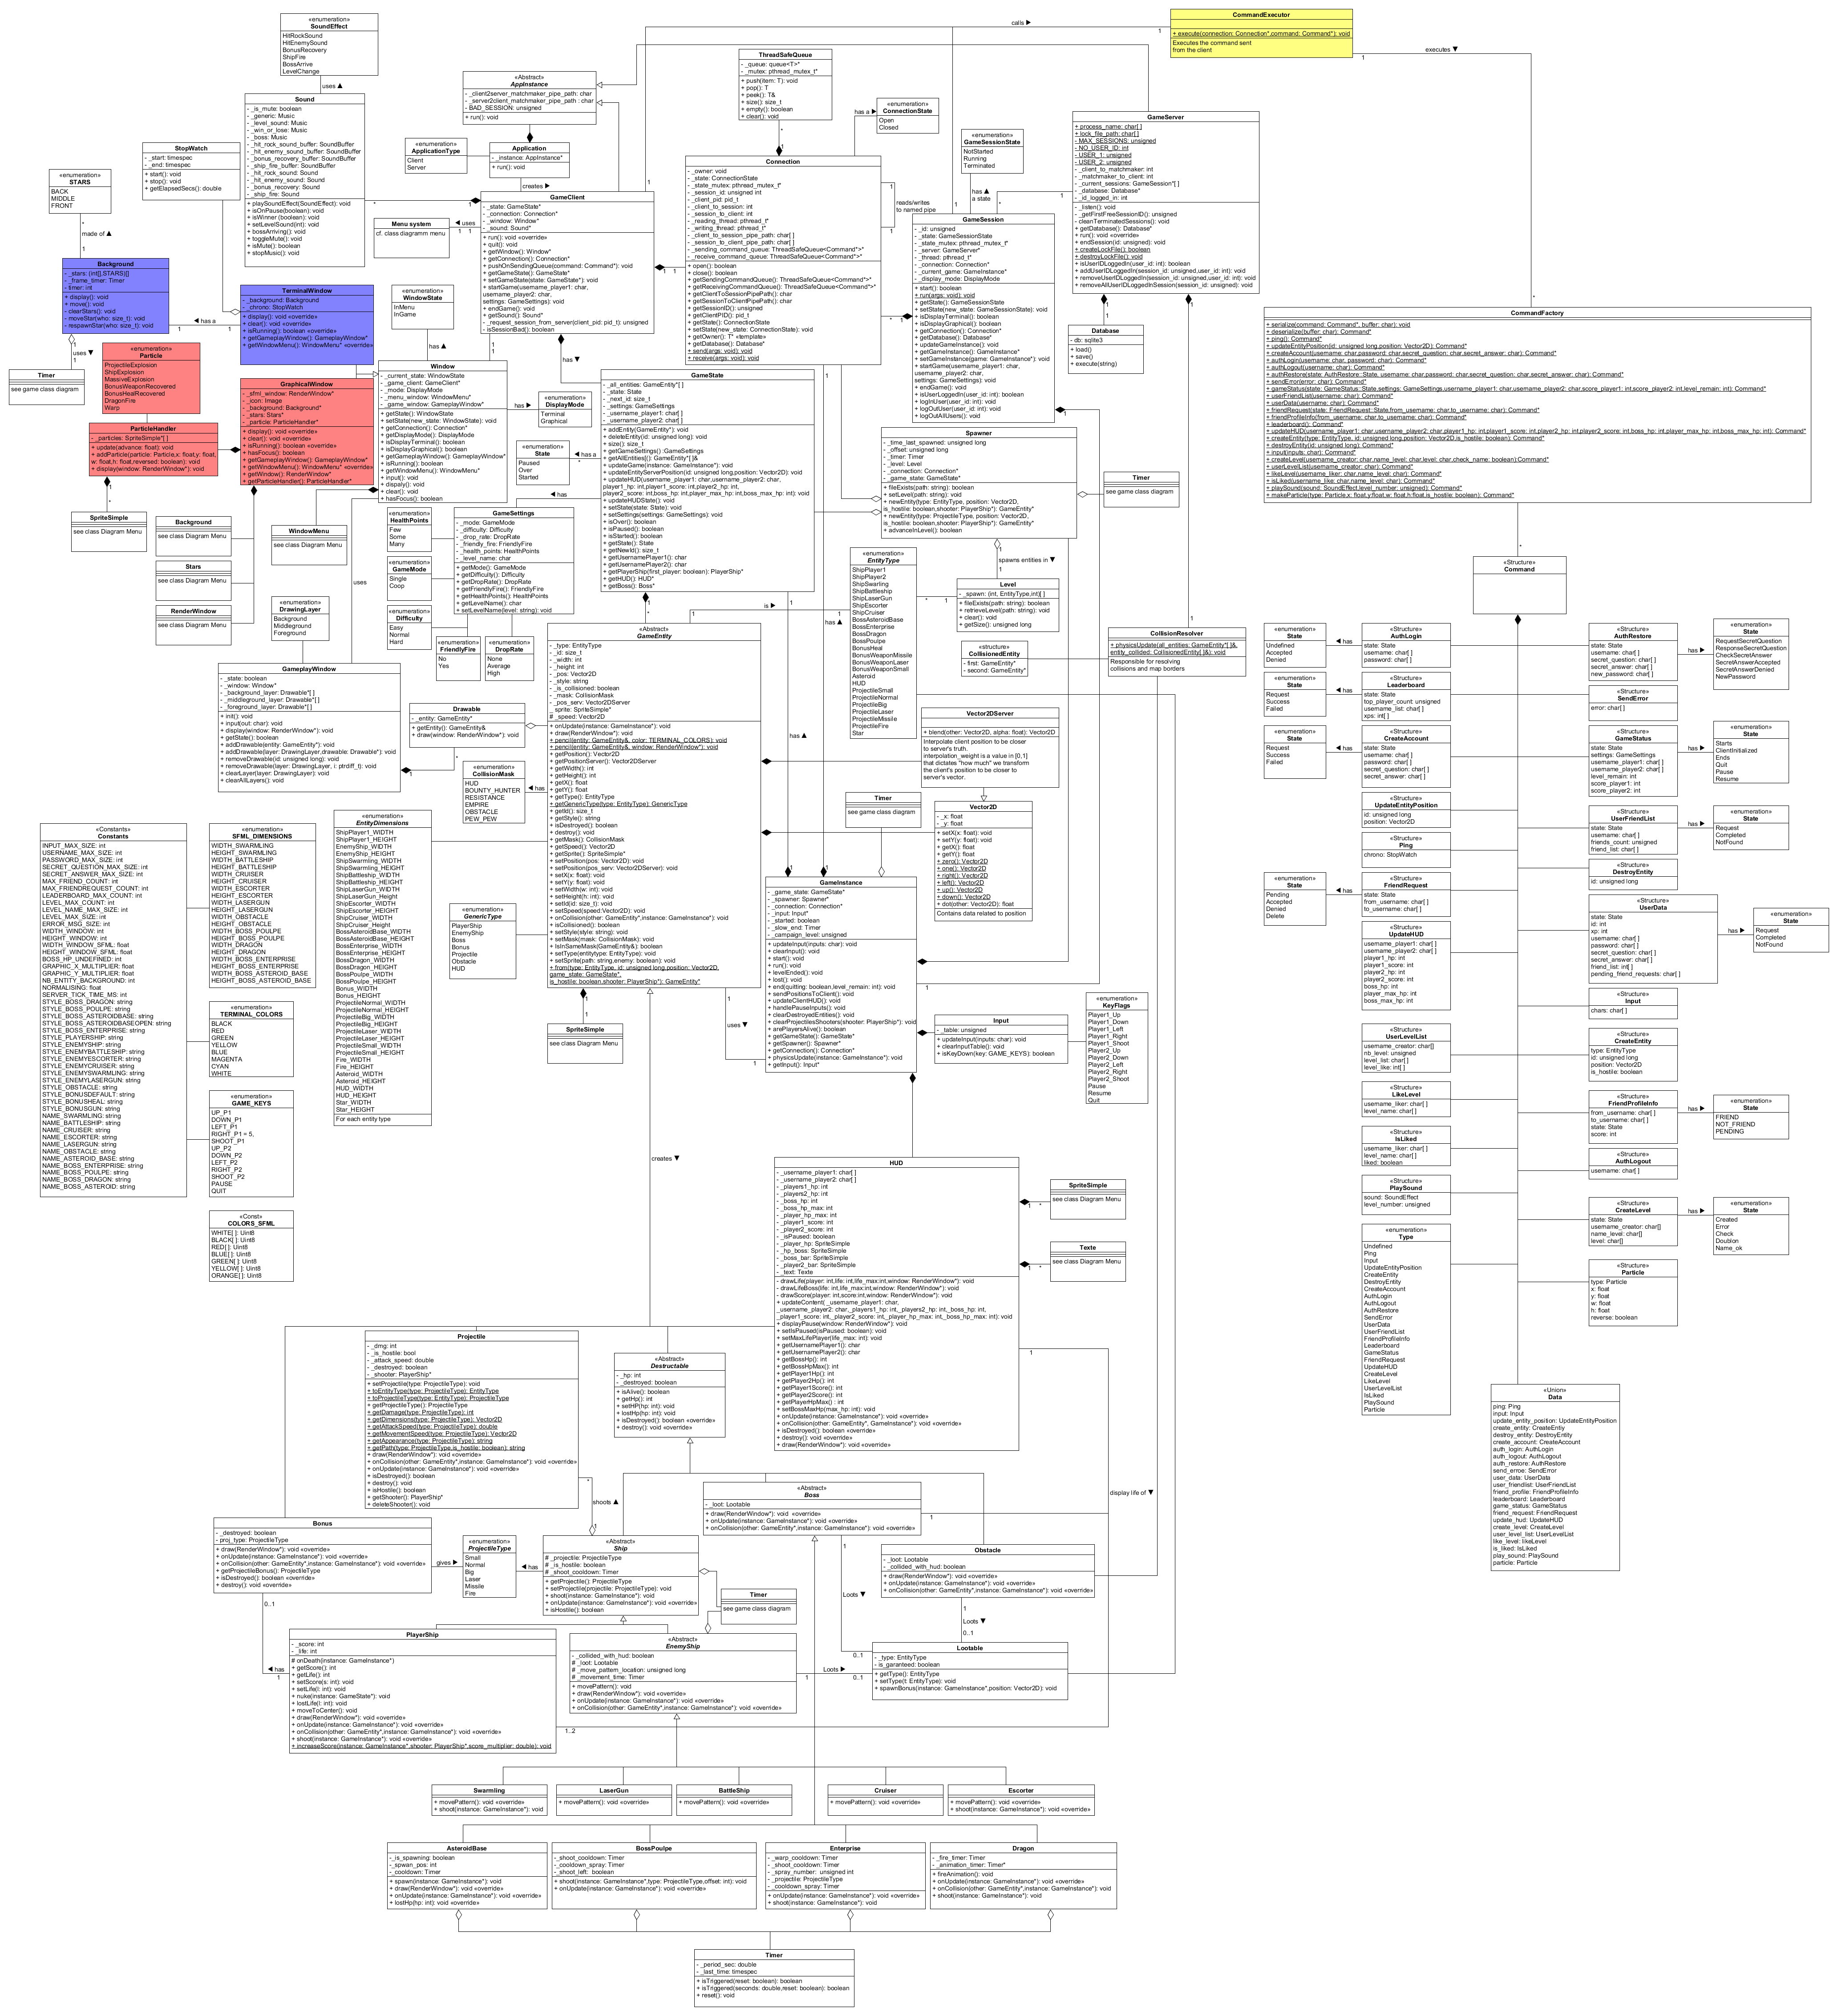
\includegraphics[scale=0.11, angle=90]{class_diagram/class_diagramm_game.png}
    \caption{Diagramme de classe du jeu- vue d'ensemble}
    \label{class diagram:game-gameplay}
\end{figure}

\restoregeometry
\section{Screenshots}
\begin{figure}[!htbp]
\subfloat[Connection window Ncurses]{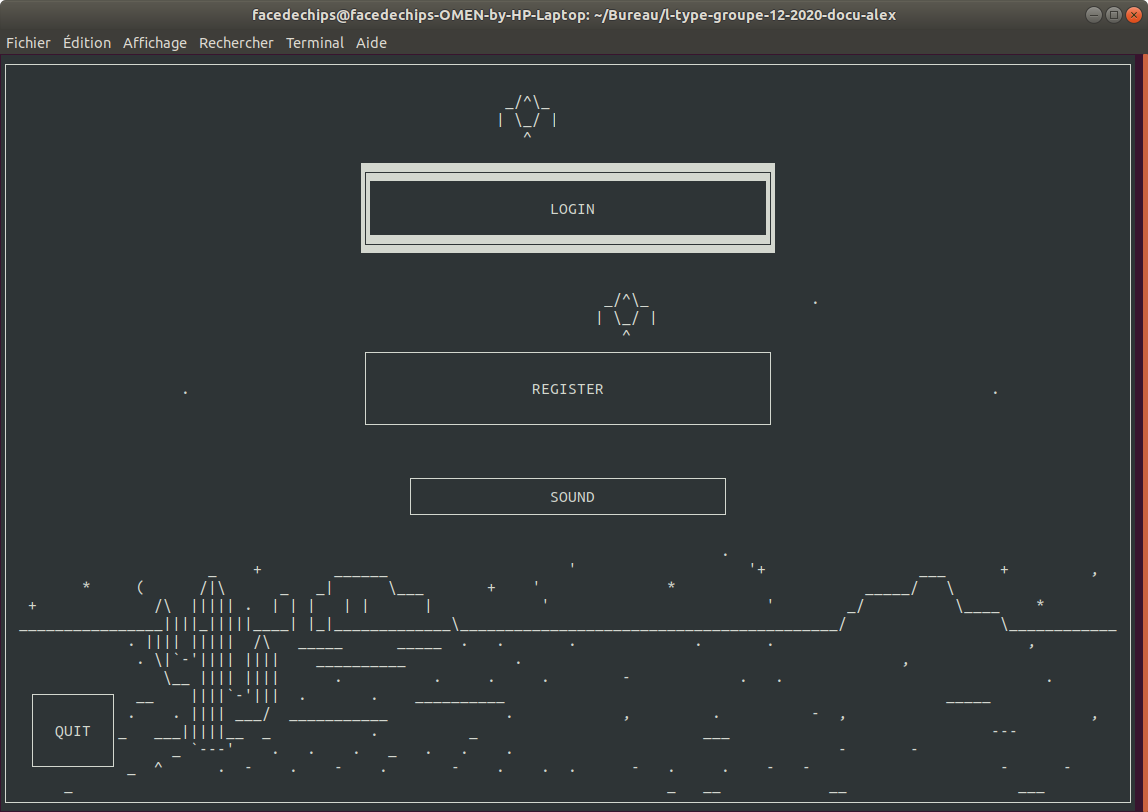
\includegraphics[scale=0.199,angle=0]{Screenshots/NCURSES/login_register_menu_ncurses.png}}
\subfloat[Connection window SFML]{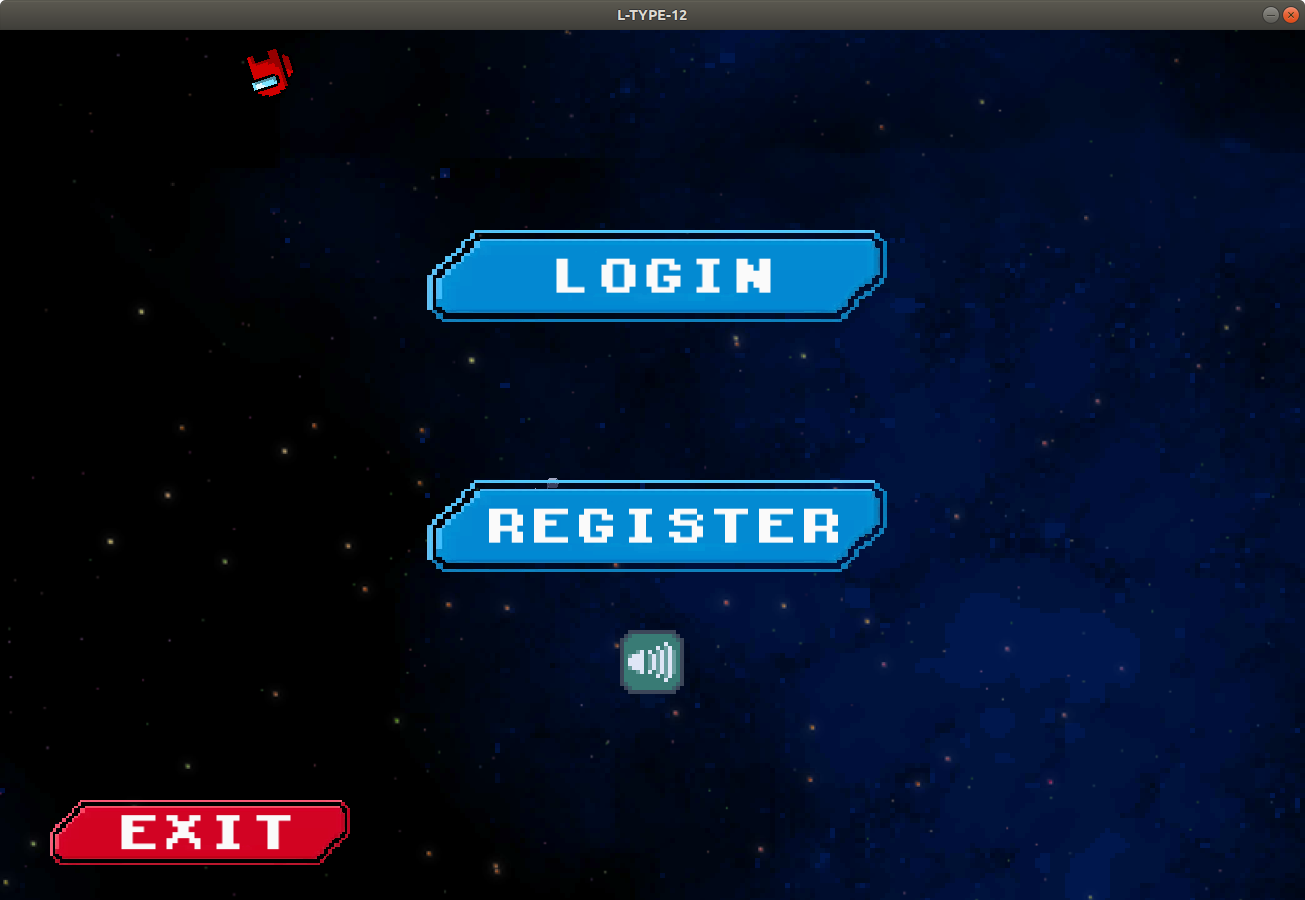
\includegraphics[scale=0.18, angle=0]{Screenshots/SFML/login_register_menu.png}}\\
\subfloat[Login view Ncurses]{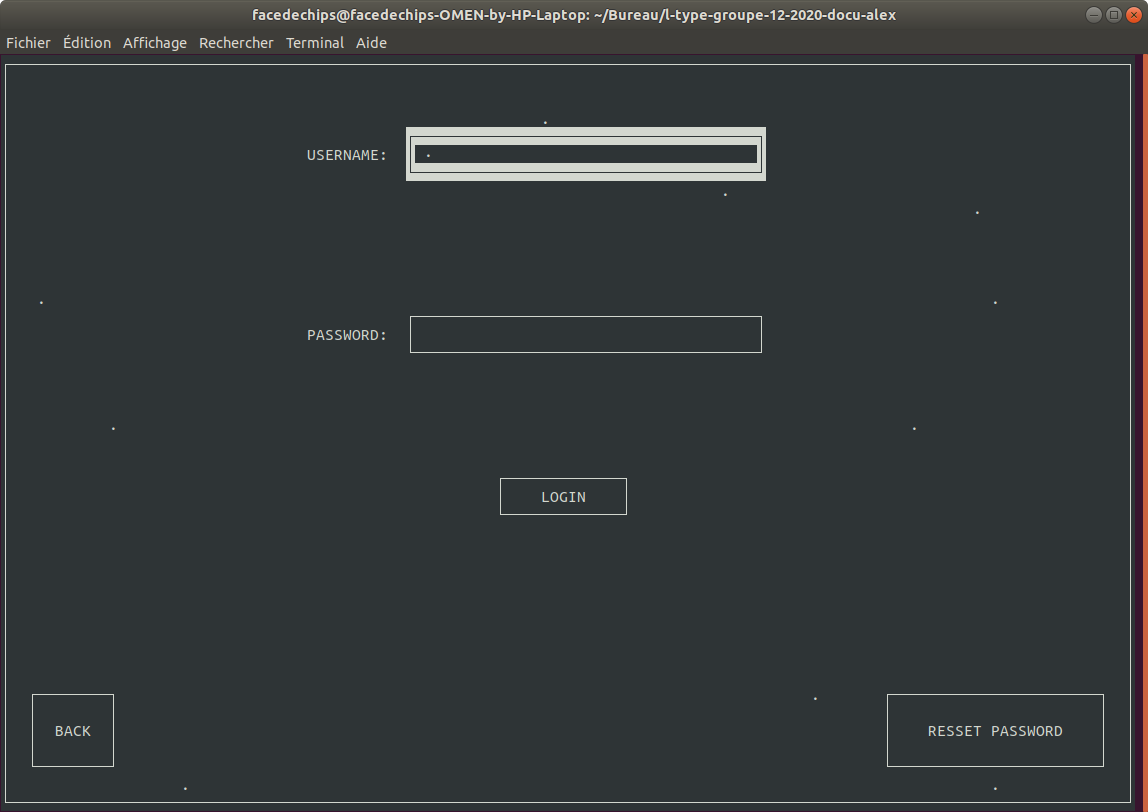
\includegraphics[scale=0.199,angle=0]{Screenshots/NCURSES/login_menu_ncurses.png}}
\subfloat[Login view SFML]{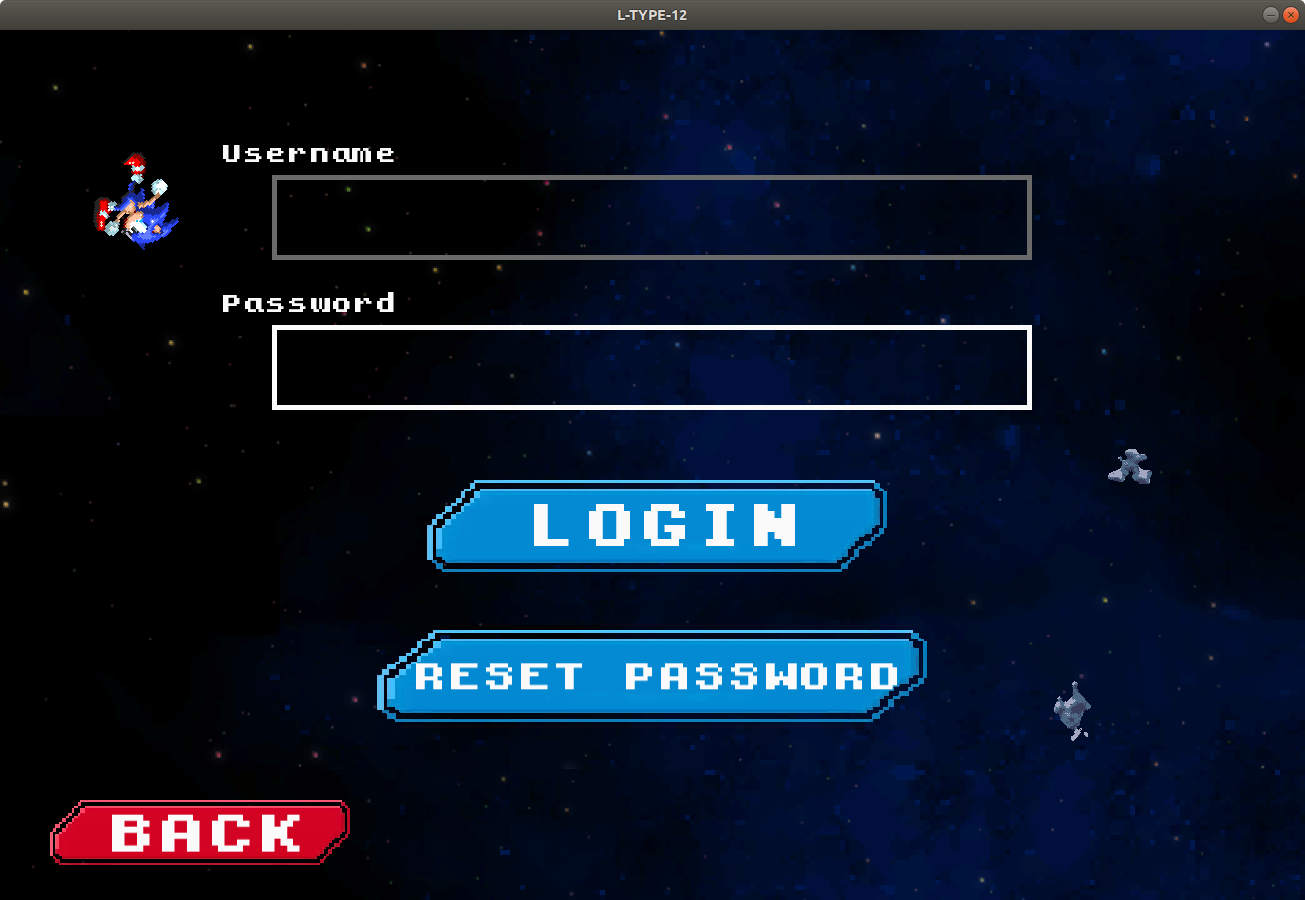
\includegraphics[scale=0.18, angle=0]{Screenshots/SFML/login_menu.png}}\\
\subfloat[Reset password Ncurses(1)]{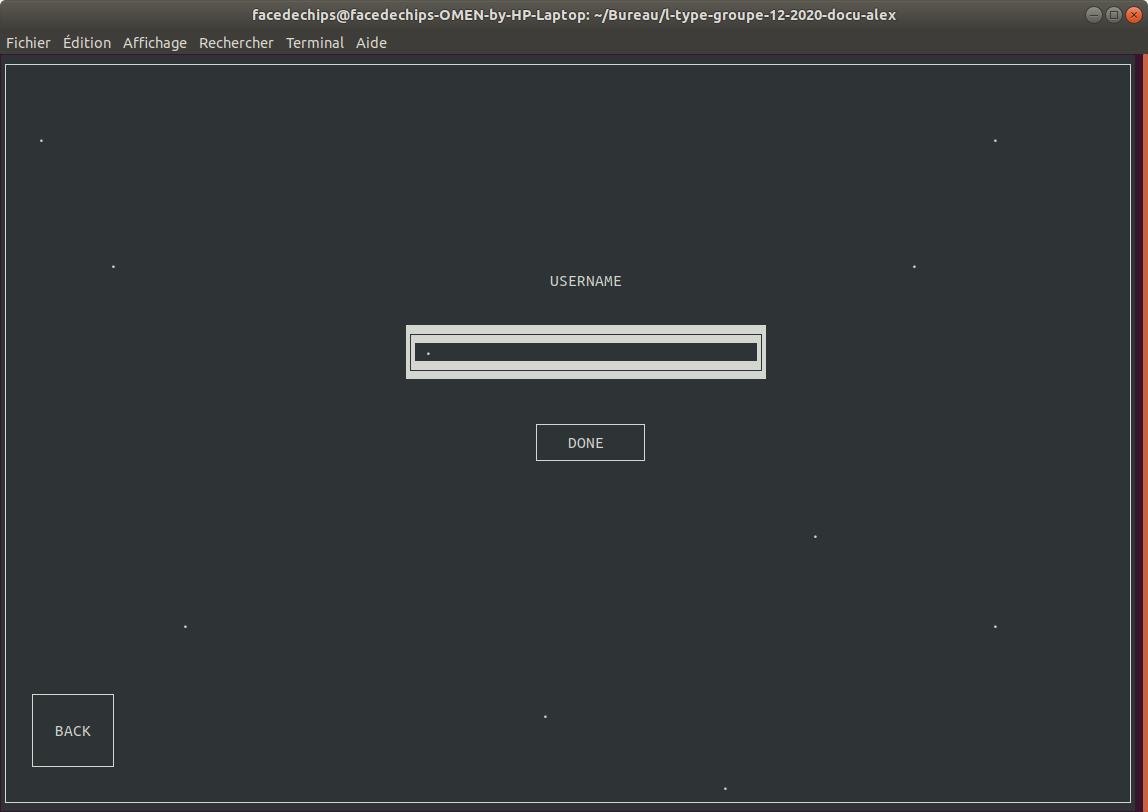
\includegraphics[scale=0.199,angle=0]{Screenshots/NCURSES/reset_password_username_menu_ncurses.png}}
\subfloat[Reset password SFML(1)]{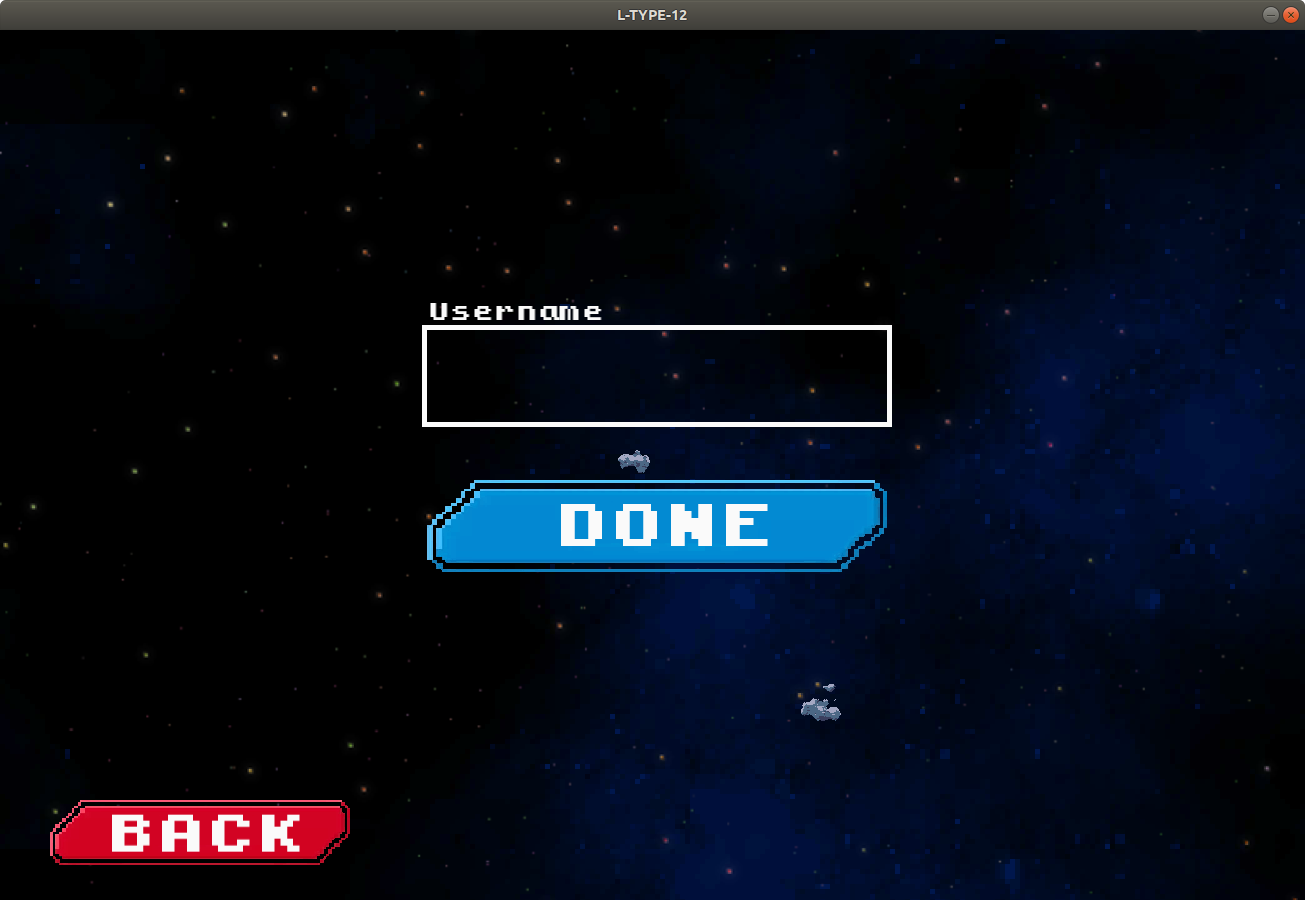
\includegraphics[scale=0.18, angle=0]{Screenshots/SFML/reset_password_username_menu.png}}\\
\end{figure}
\begin{figure}[!htbp]
\subfloat[Reset password Ncurses(2]{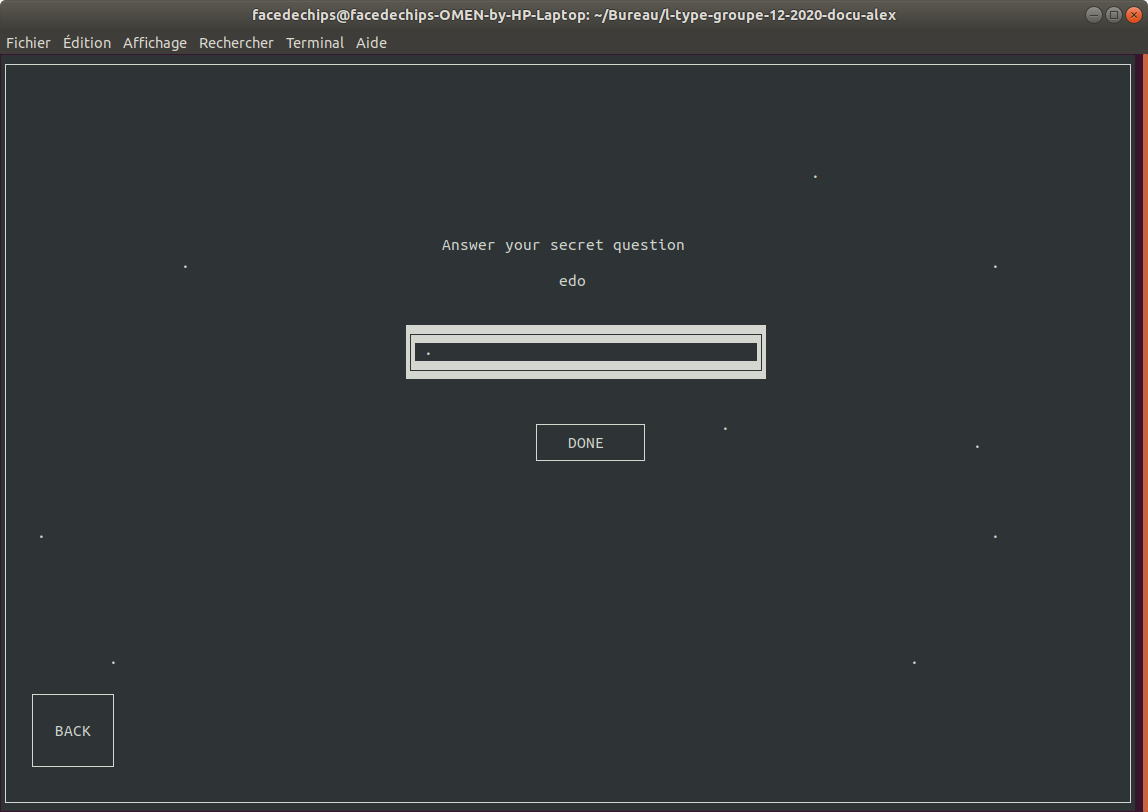
\includegraphics[scale=0.199,angle=0]{Screenshots/NCURSES/reset_password_question_menu_ncurses.png}}
\subfloat[Reset password SFML(2)]{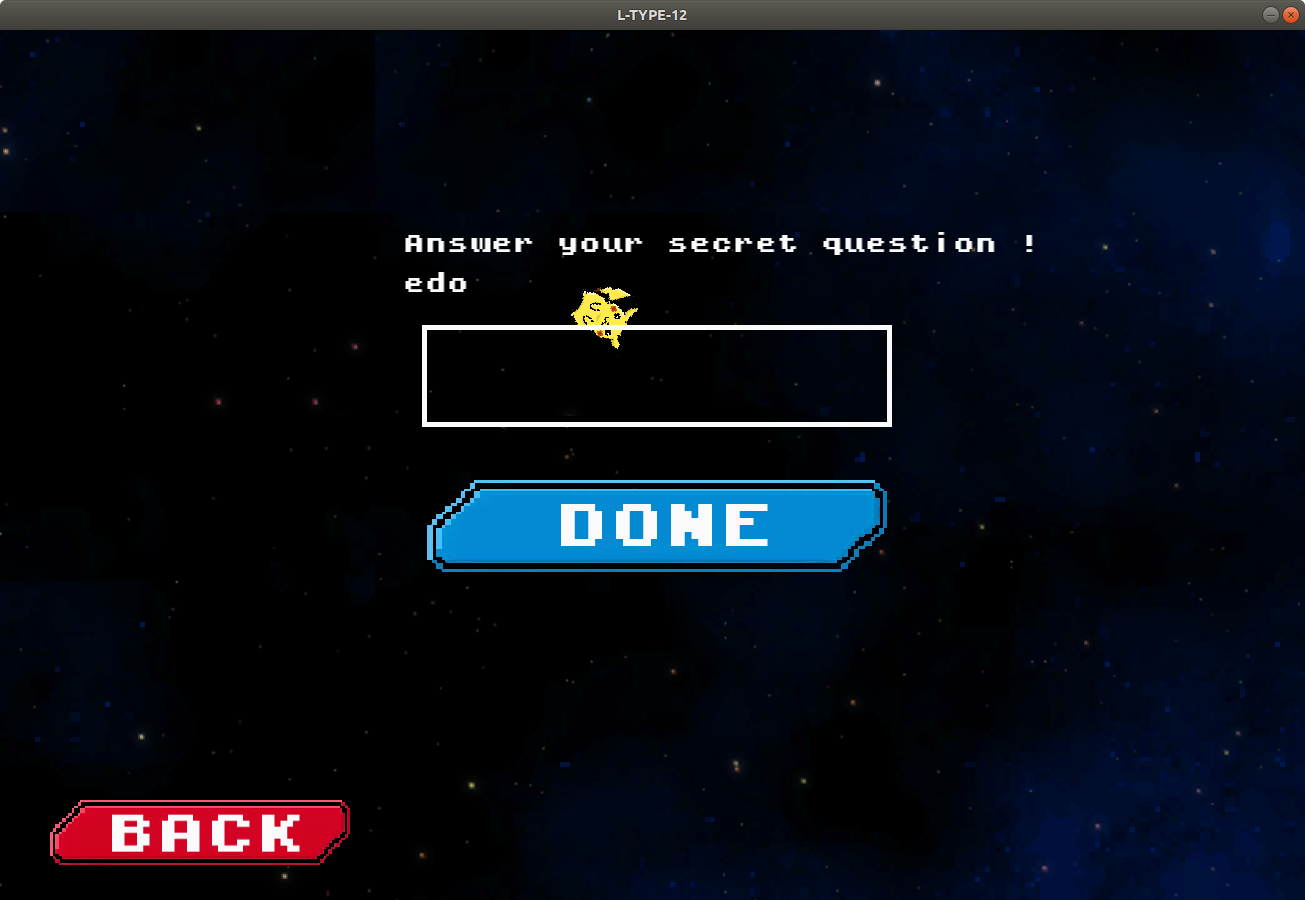
\includegraphics[scale=0.18, angle=0]{Screenshots/SFML/reset_password_question_menu.png}}\\
\subfloat[Reset password Ncurses(3)]{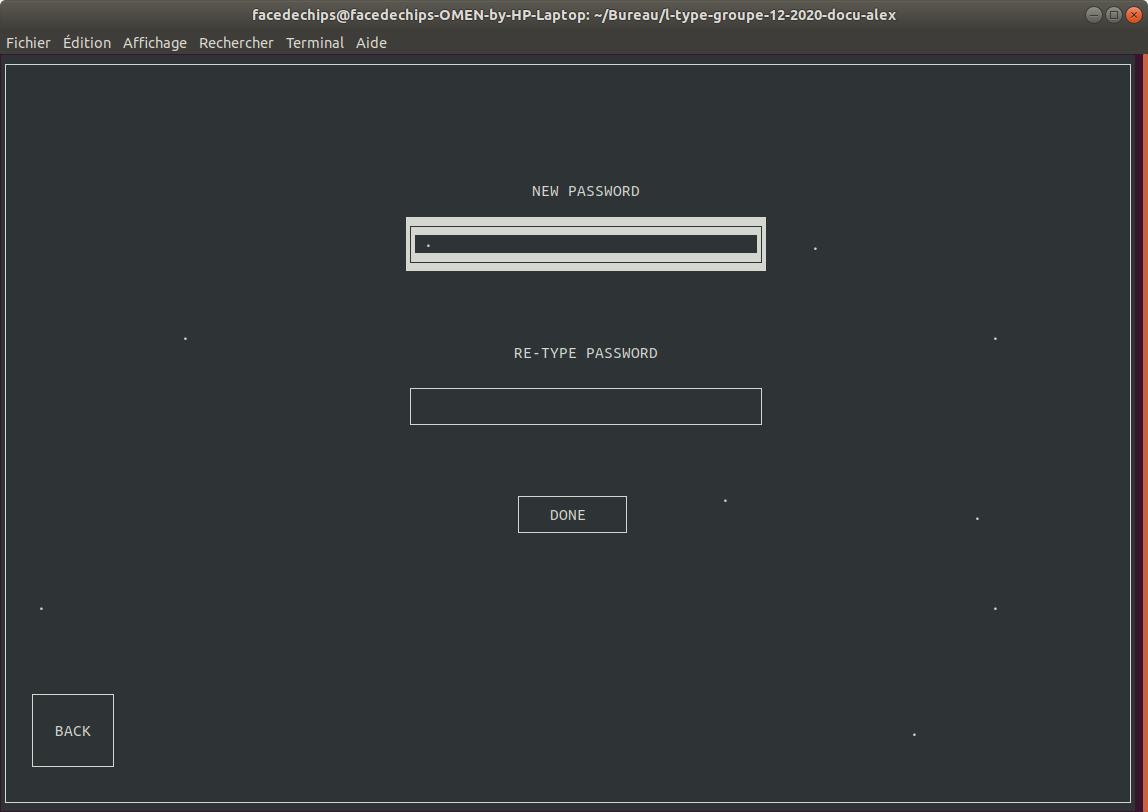
\includegraphics[scale=0.199,angle=0]{Screenshots/NCURSES/reset_password_new_password_menu_ncurses.png}}
\subfloat[Reset password SFML(3)]{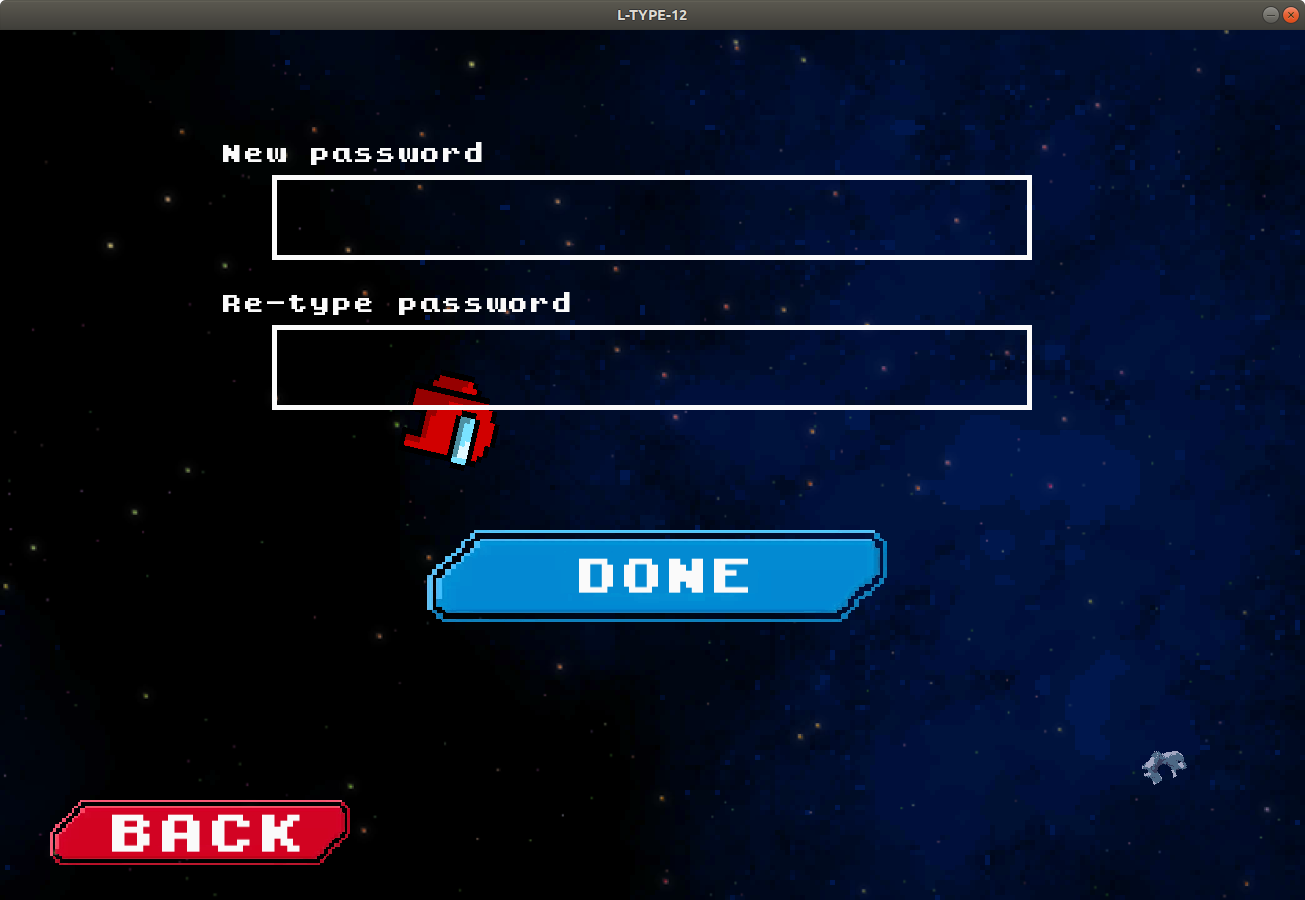
\includegraphics[scale=0.18, angle=0]{Screenshots/SFML/reset_password_new_password_menu.png}}\\
\subfloat[Register view Ncurses]{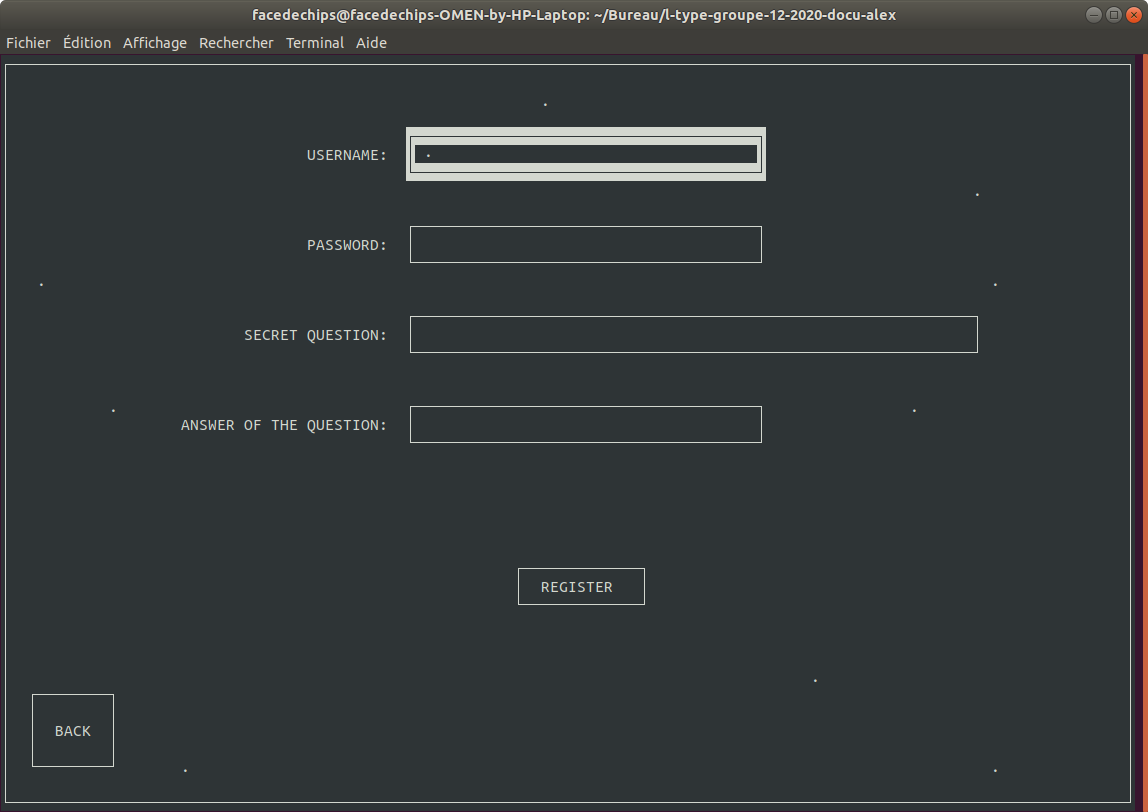
\includegraphics[scale=0.199,angle=0]{Screenshots/NCURSES/register_menu_ncurses.png}}
\subfloat[Register View SFML]{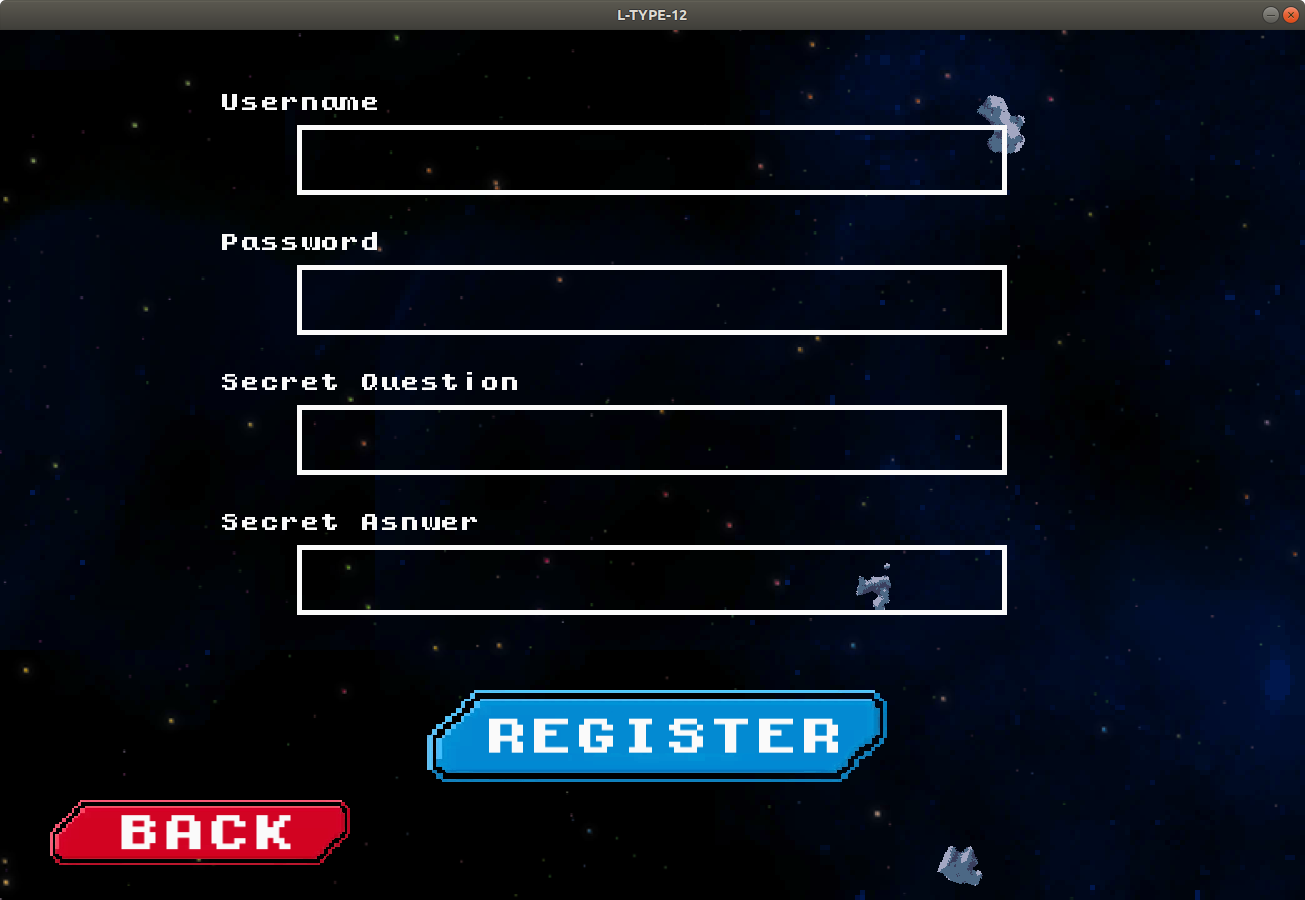
\includegraphics[scale=0.18, angle=0]{Screenshots/SFML/register_menu.png}}\\
\end{figure}
\begin{figure}[!htbp]
\subfloat[Main menu Ncurses]{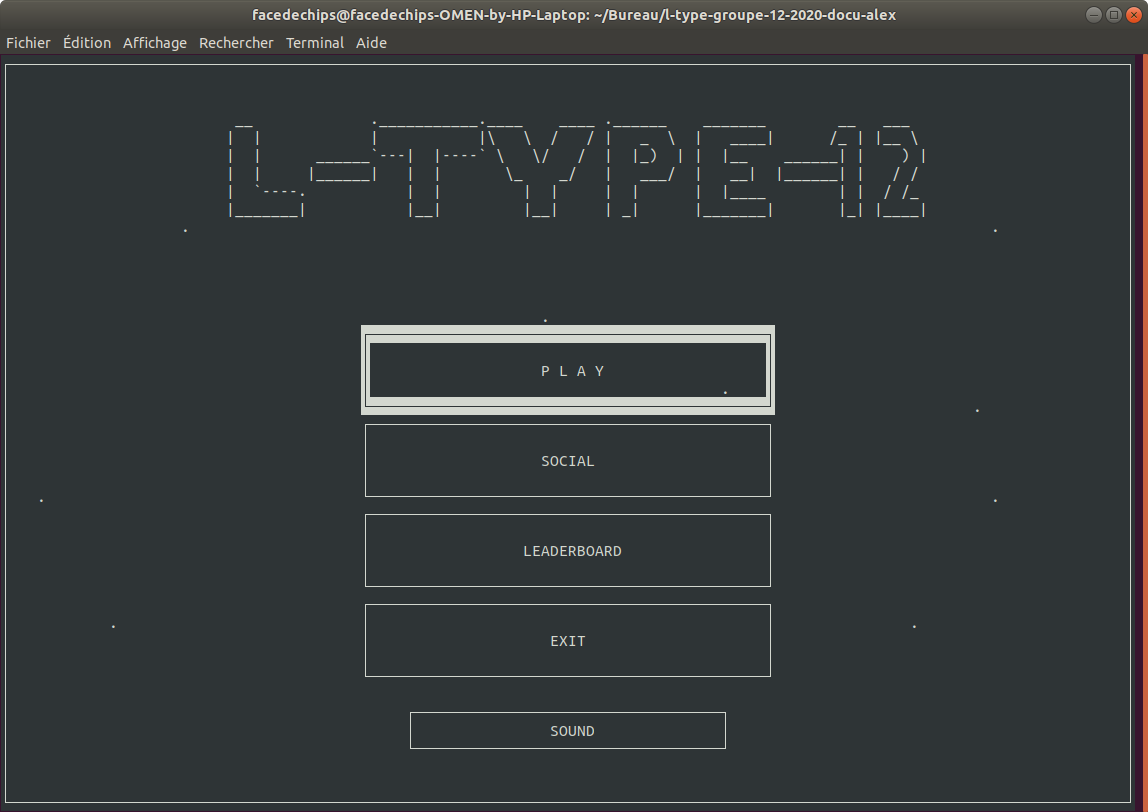
\includegraphics[scale=0.199,angle=0]{Screenshots/NCURSES/main_menu_ncurses.png}}
\subfloat[Main menu SFML]{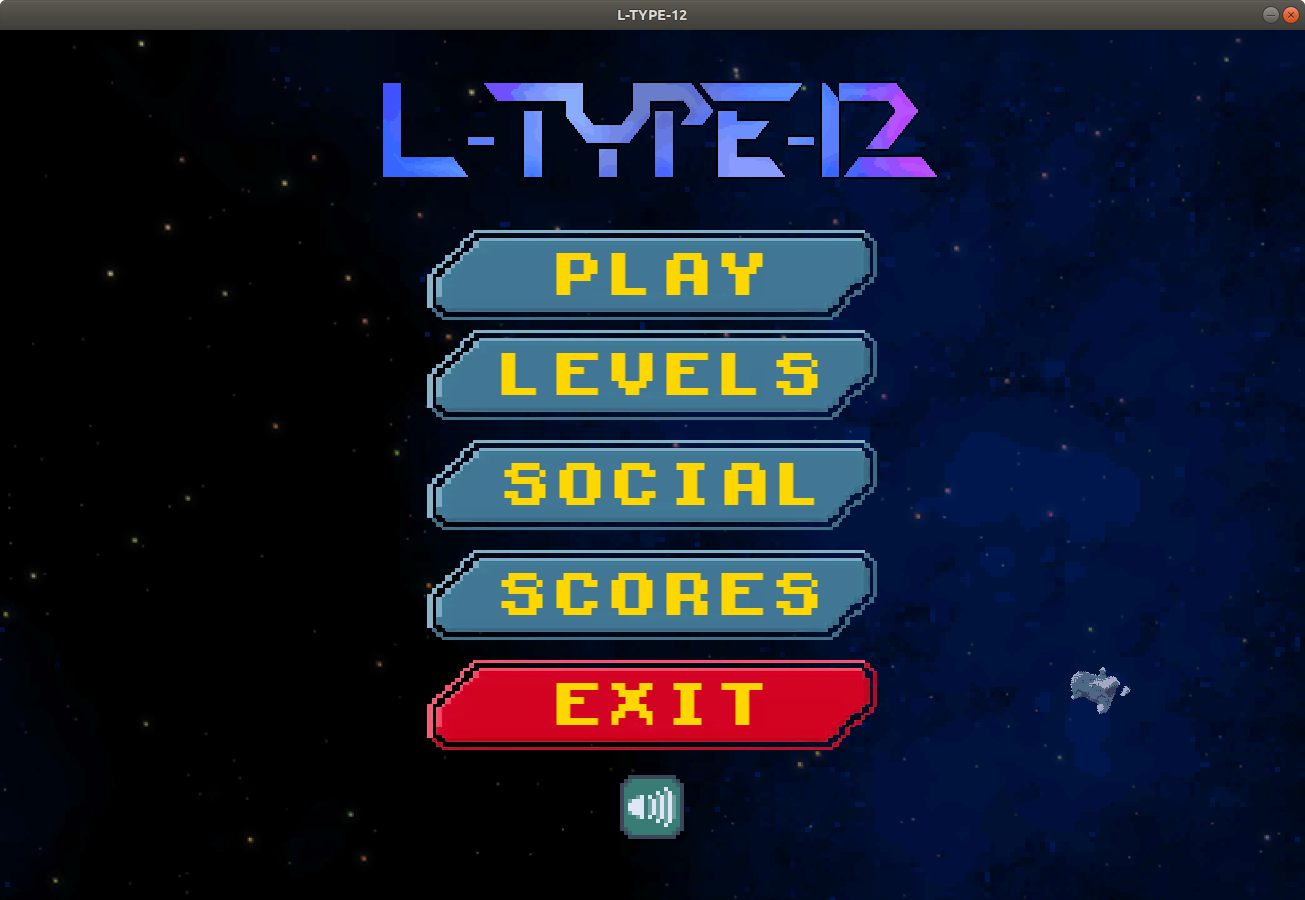
\includegraphics[scale=0.18, angle=0]{Screenshots/SFML/main_menu.png}}\\
\subfloat[Room menu Ncurses]{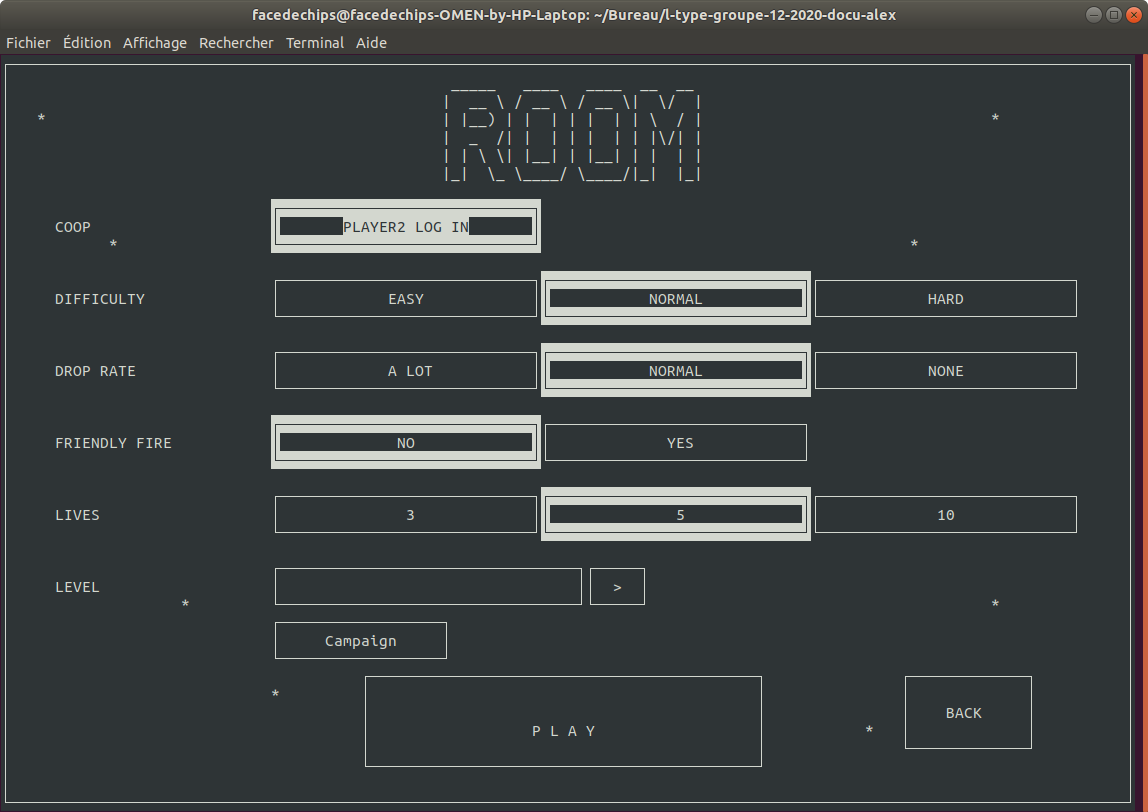
\includegraphics[scale=0.199,angle=0]{Screenshots/NCURSES/room_menu_ncurses.png}}
\subfloat[Romm menu SFML]{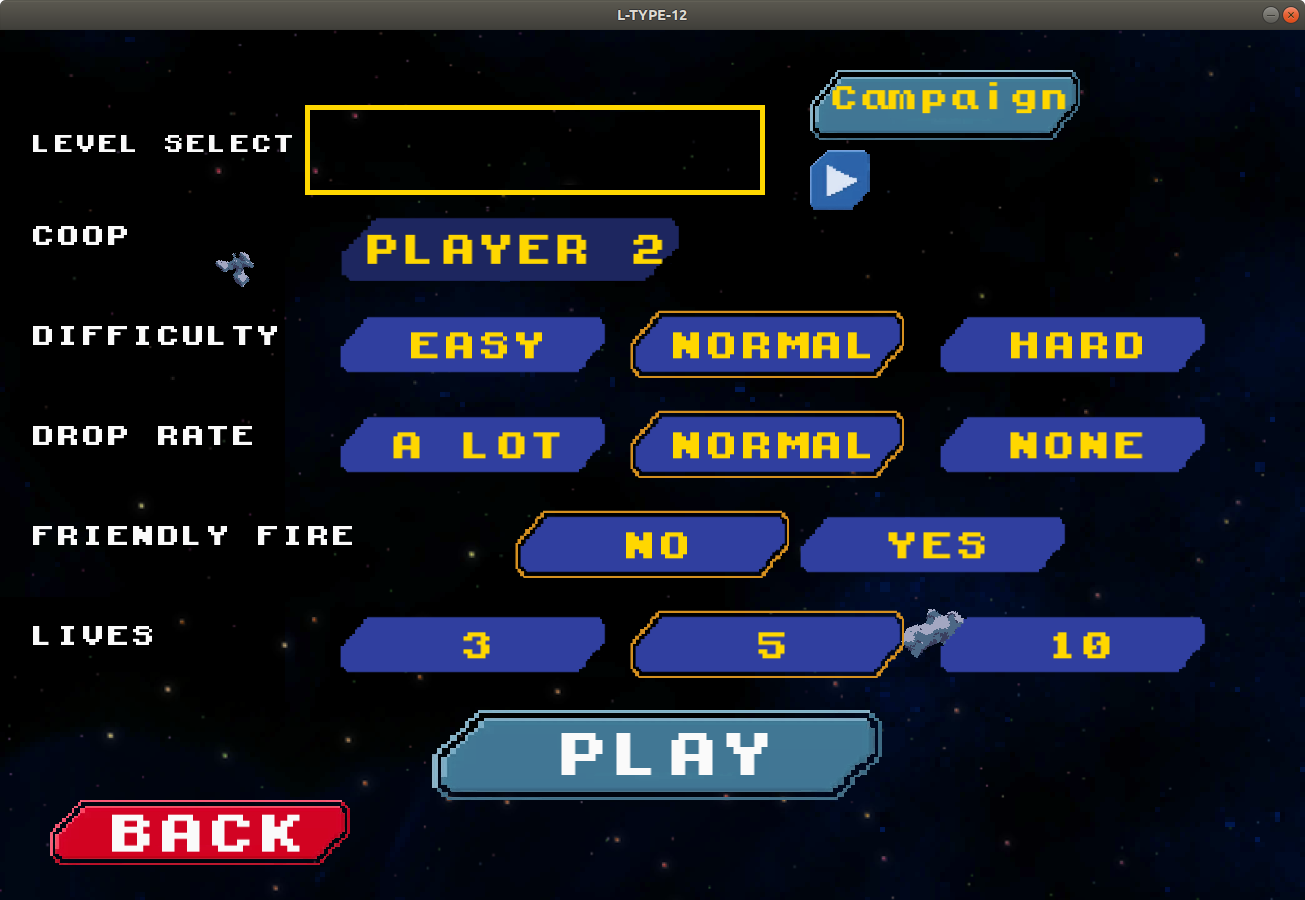
\includegraphics[scale=0.18, angle=0]{Screenshots/SFML/room_menu.png}}\\
\subfloat[Leaderboard menu Ncurses]{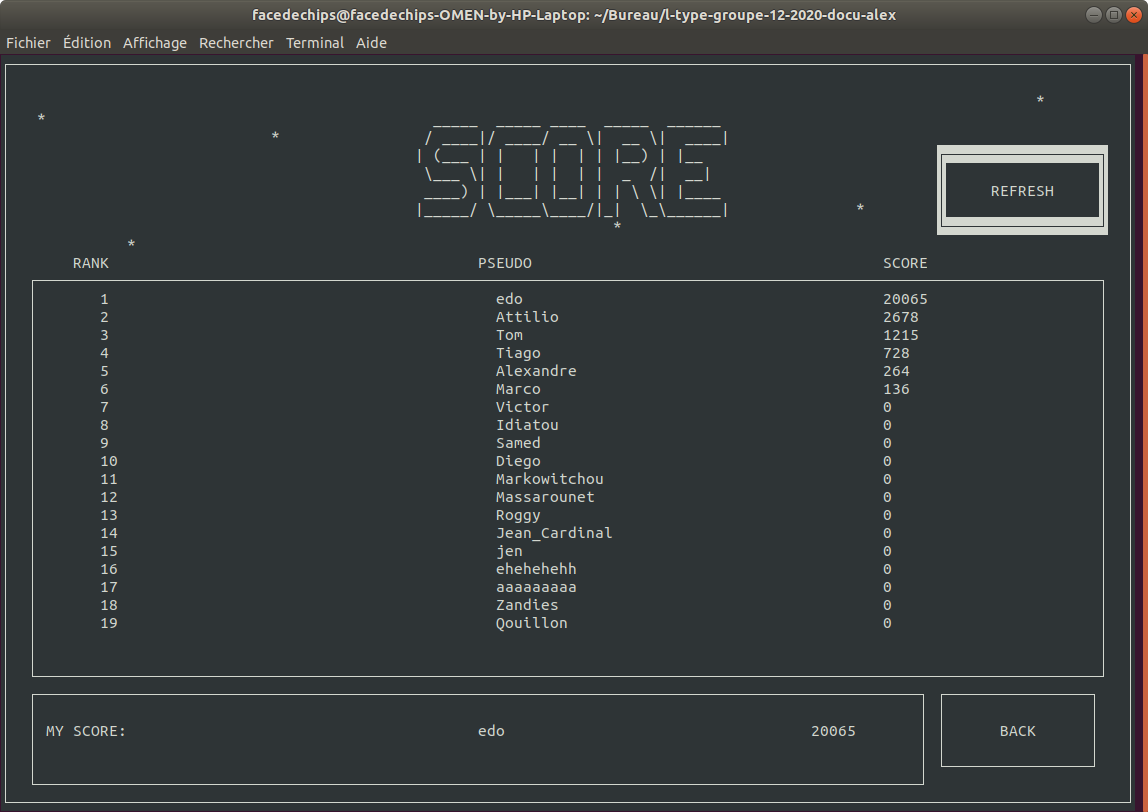
\includegraphics[scale=0.199,angle=0]{Screenshots/NCURSES/leaderboard_menu_ncurses.png}}
\subfloat[Leaderboard menu SFML]{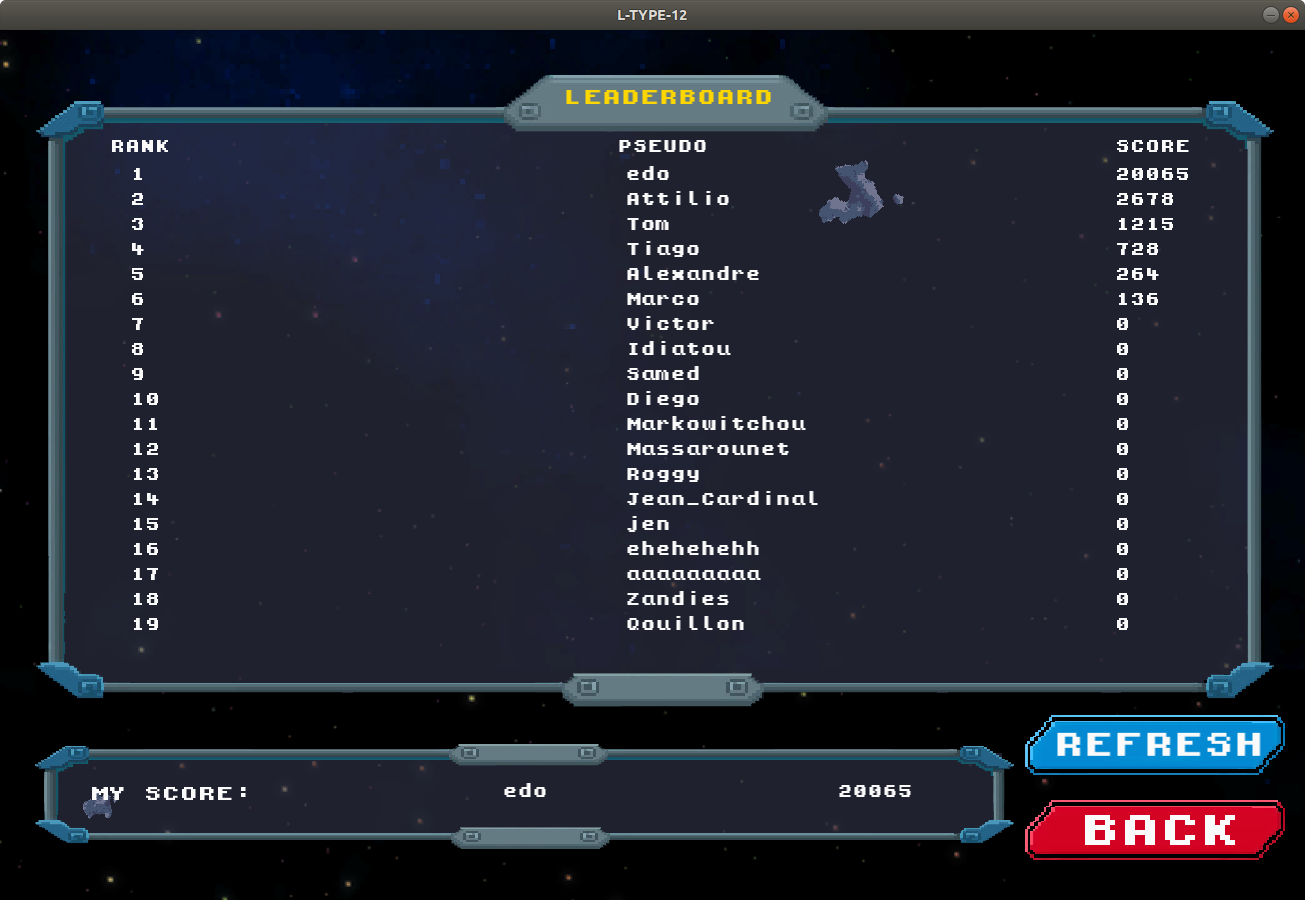
\includegraphics[scale=0.18, angle=0]{Screenshots/SFML/leaderboard_menu.png}}\\
\end{figure}
\begin{figure}[!htbp]
\subfloat[Social menu Ncurses]{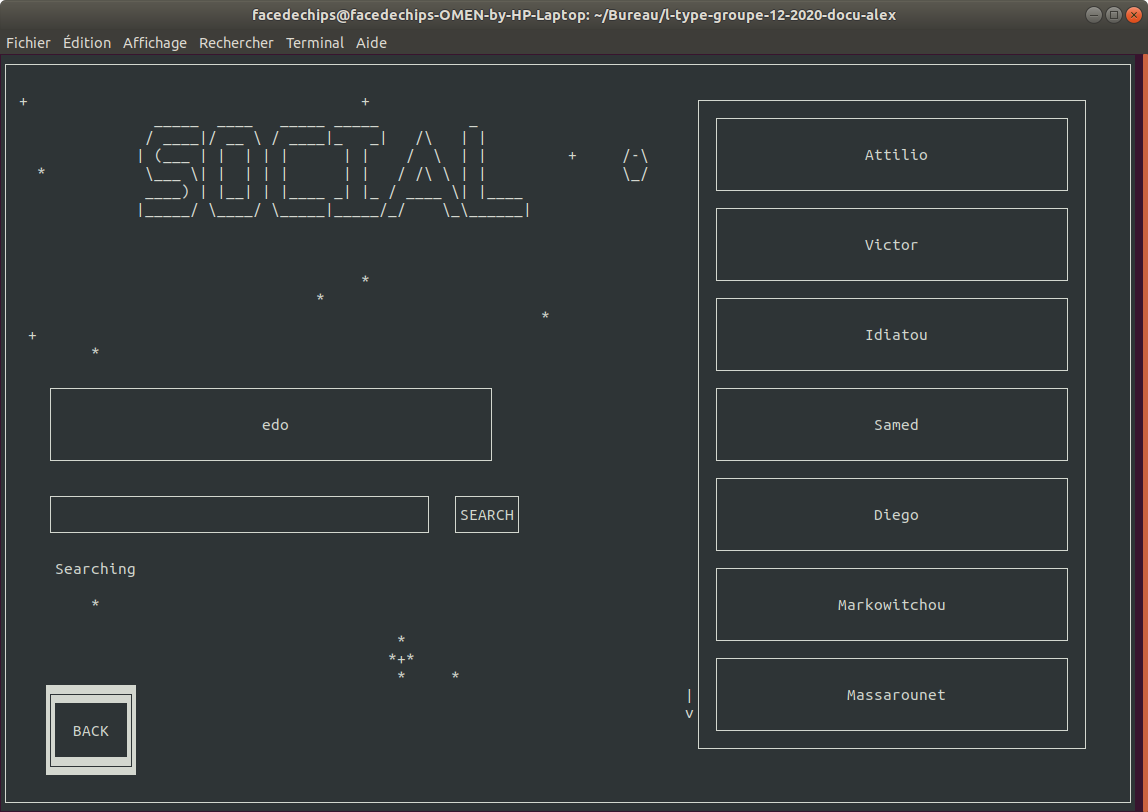
\includegraphics[scale=0.199,angle=0]{Screenshots/NCURSES/social_menu_ncurses.png}}
\subfloat[Social menu SFML]{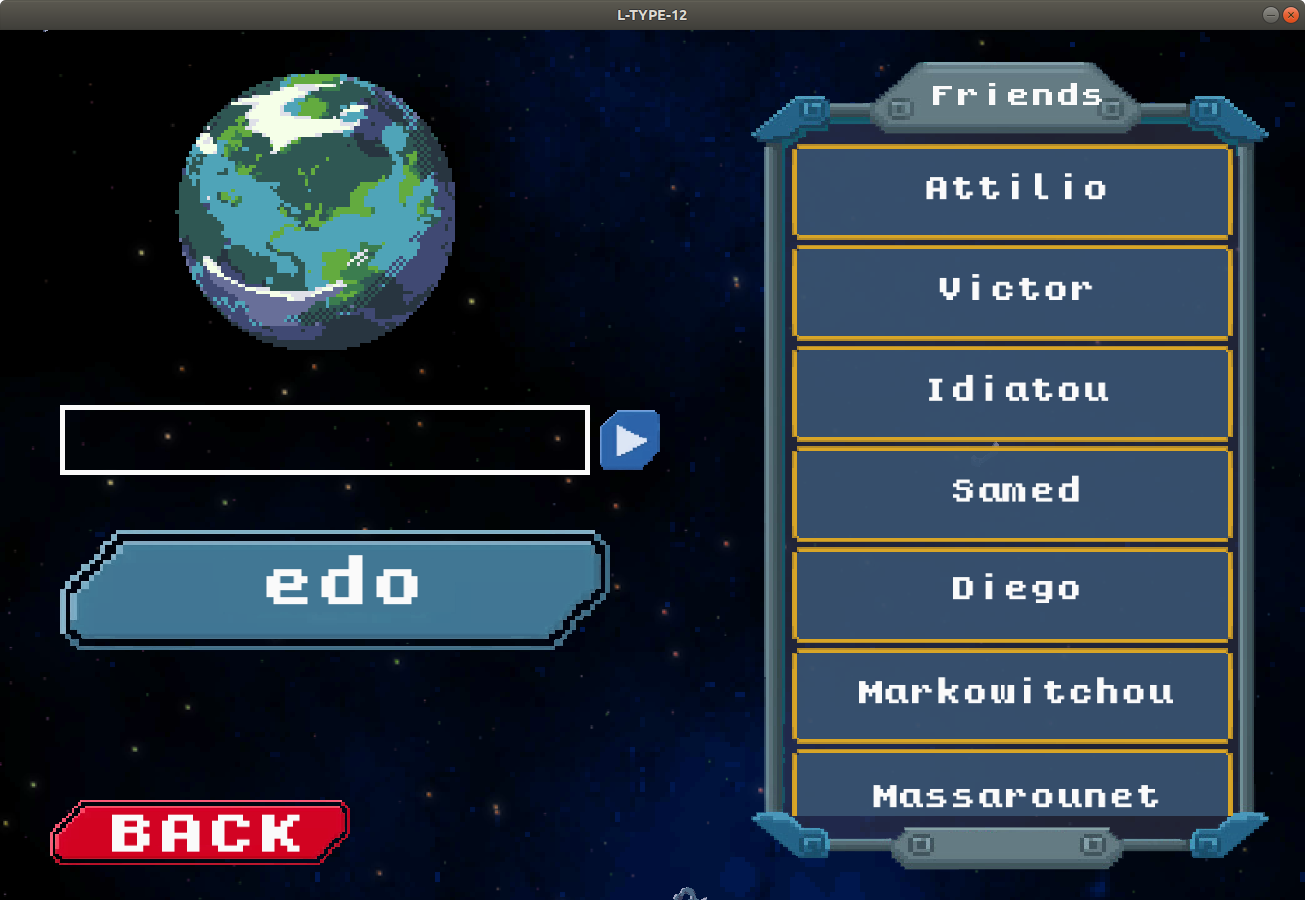
\includegraphics[scale=0.18, angle=0]{Screenshots/SFML/social_menu.png}}\\
\subfloat[My profil view Ncurses]{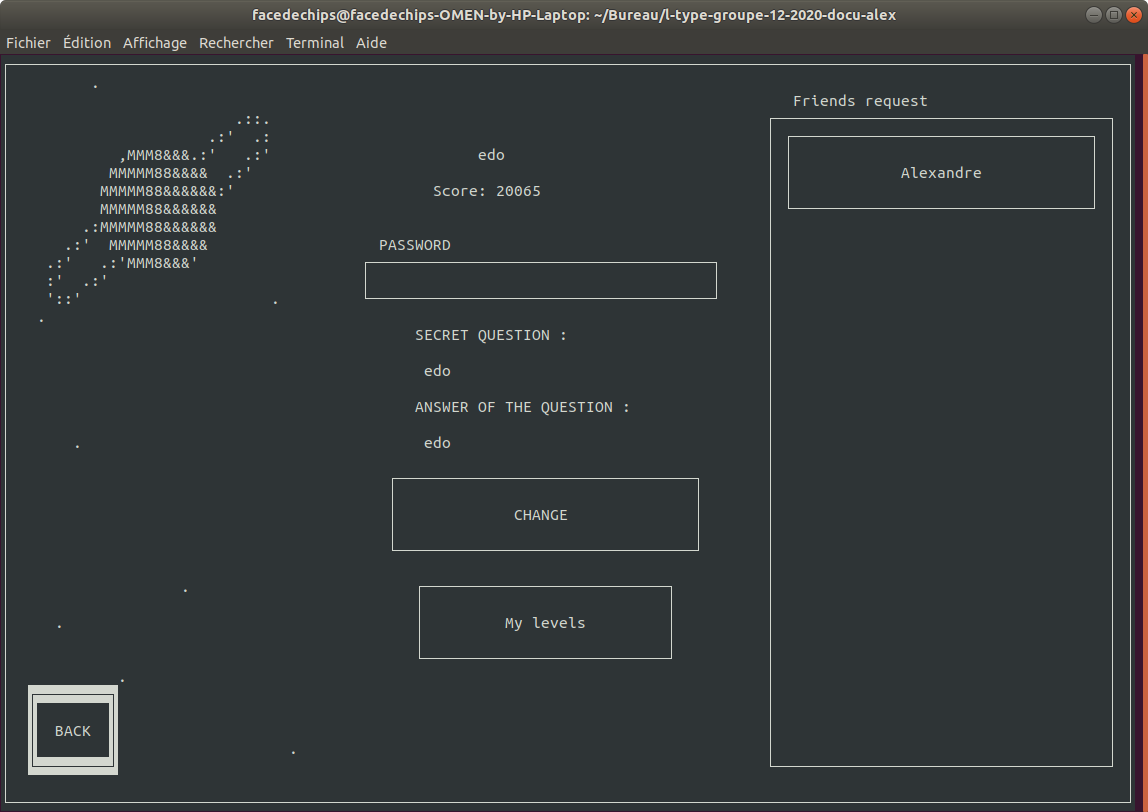
\includegraphics[scale=0.199,angle=0]{Screenshots/NCURSES/social_menu_my_profil_ncurses.png}}
\subfloat[My profil view SFML]{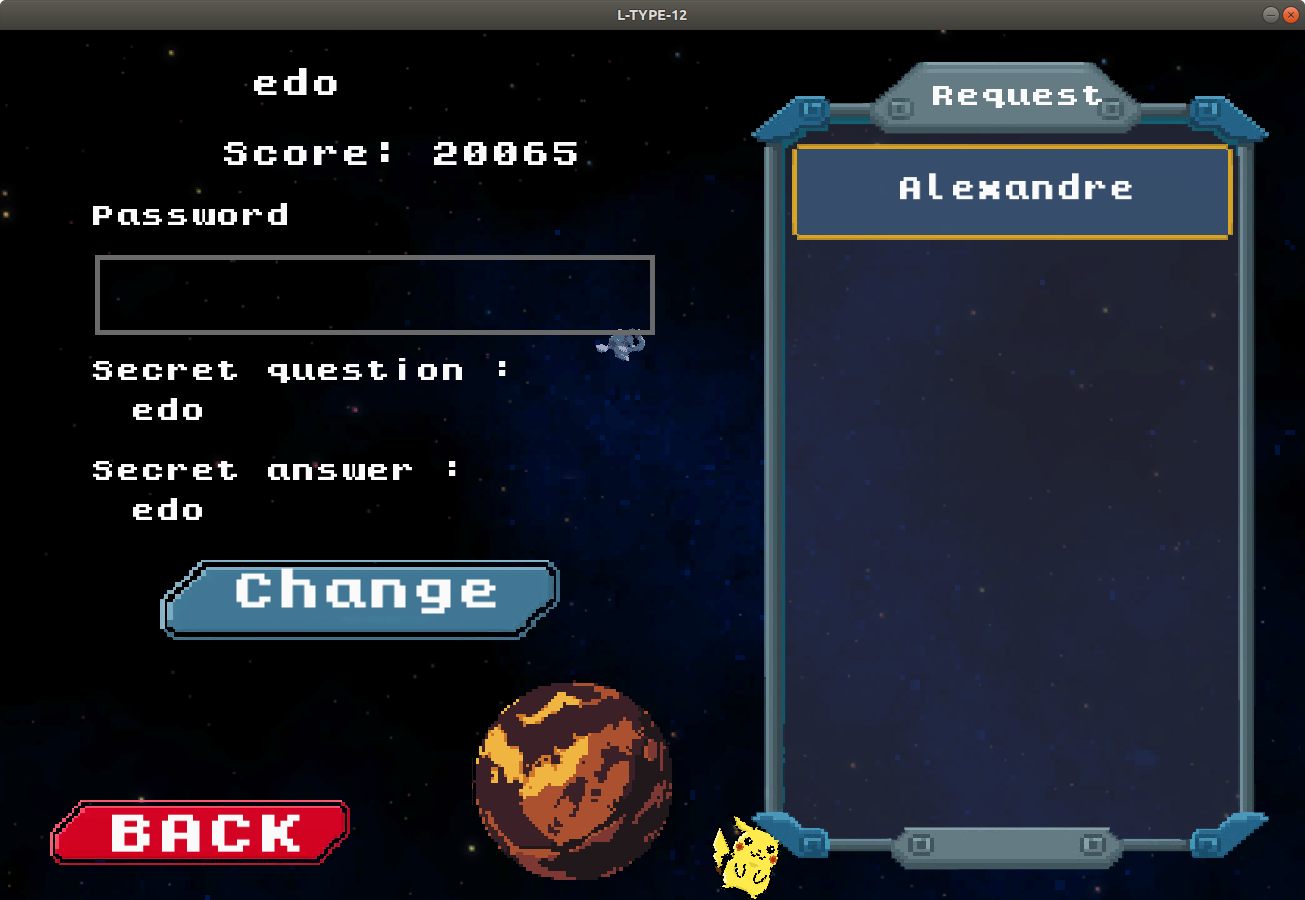
\includegraphics[scale=0.18, angle=0]{Screenshots/SFML/social_menu_my_profil.png}}\\
\subfloat[User profil view Ncurses]{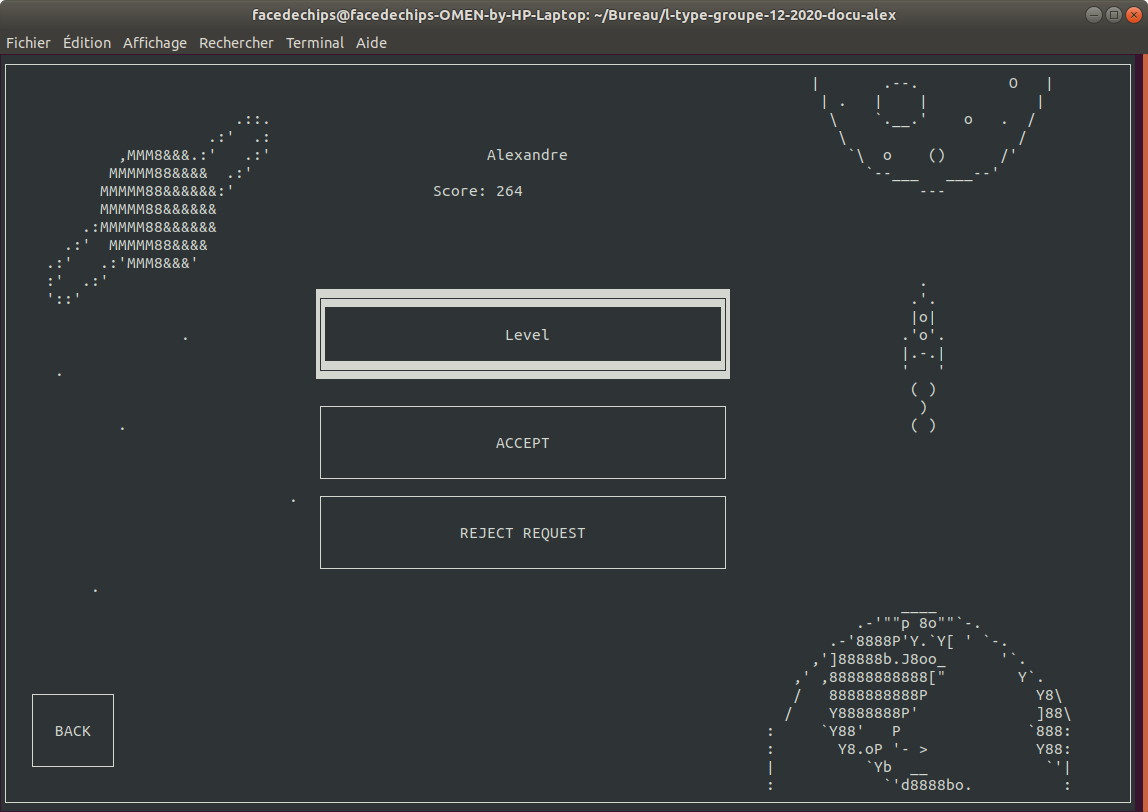
\includegraphics[scale=0.199,angle=0]{Screenshots/NCURSES/social_menu_user_profil_ncurses.png}}
\subfloat[User profil view SFML]{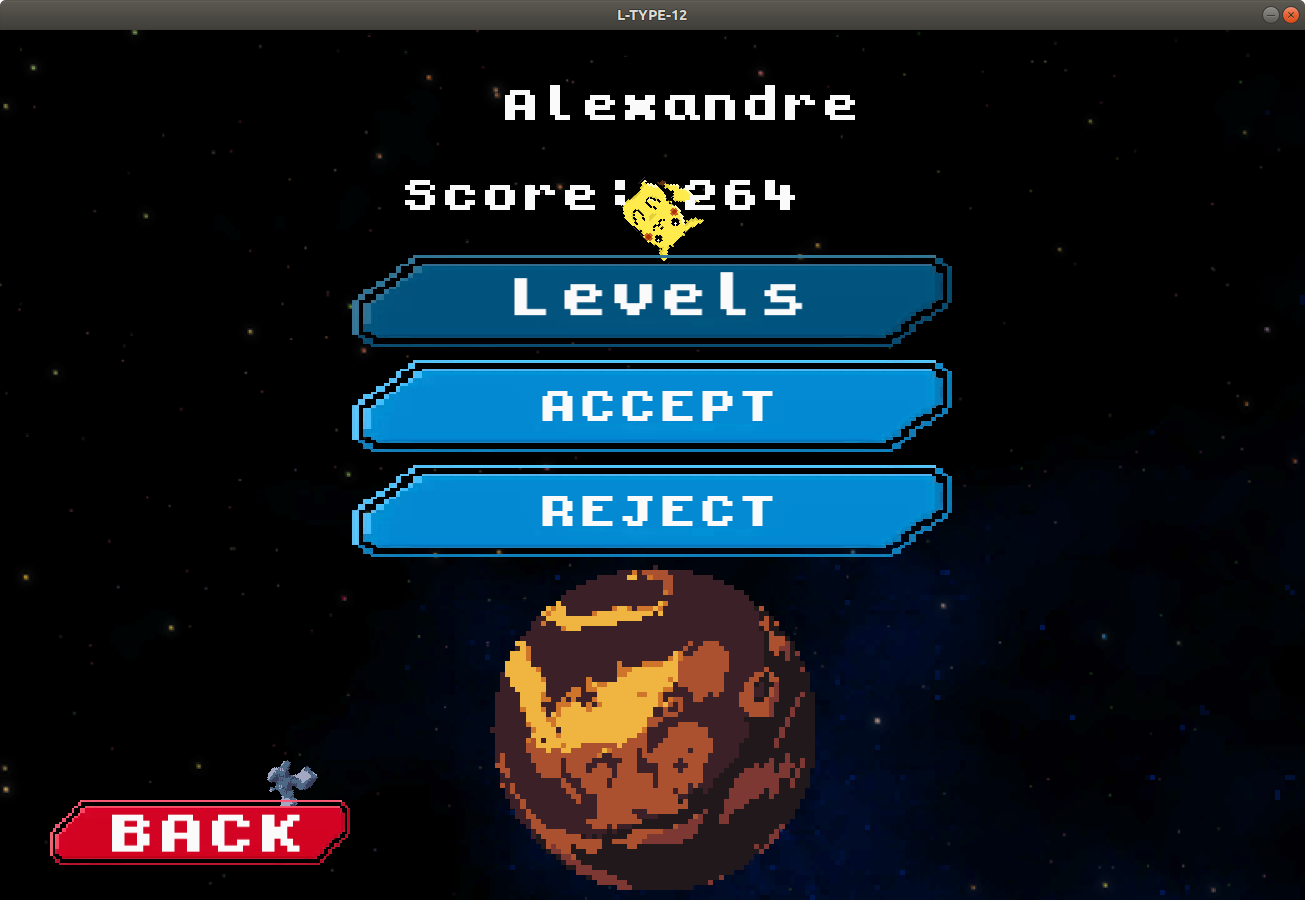
\includegraphics[scale=0.18, angle=0]{Screenshots/SFML/social_menu_user_profil.png}}\\
\end{figure}
\begin{figure}[!htbp]
\subfloat[In game view Ncurses]{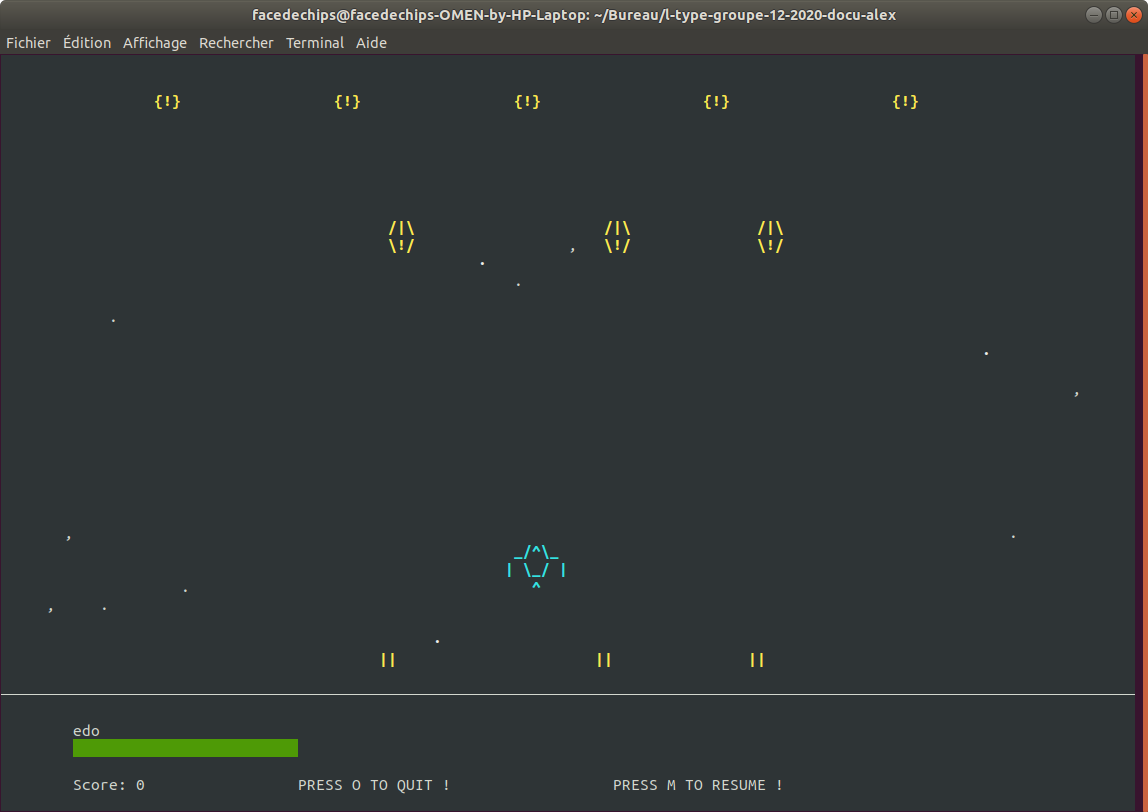
\includegraphics[scale=0.199,angle=0]{Screenshots/NCURSES/in_game_ncurses.png}}
\subfloat[In game view SFML]{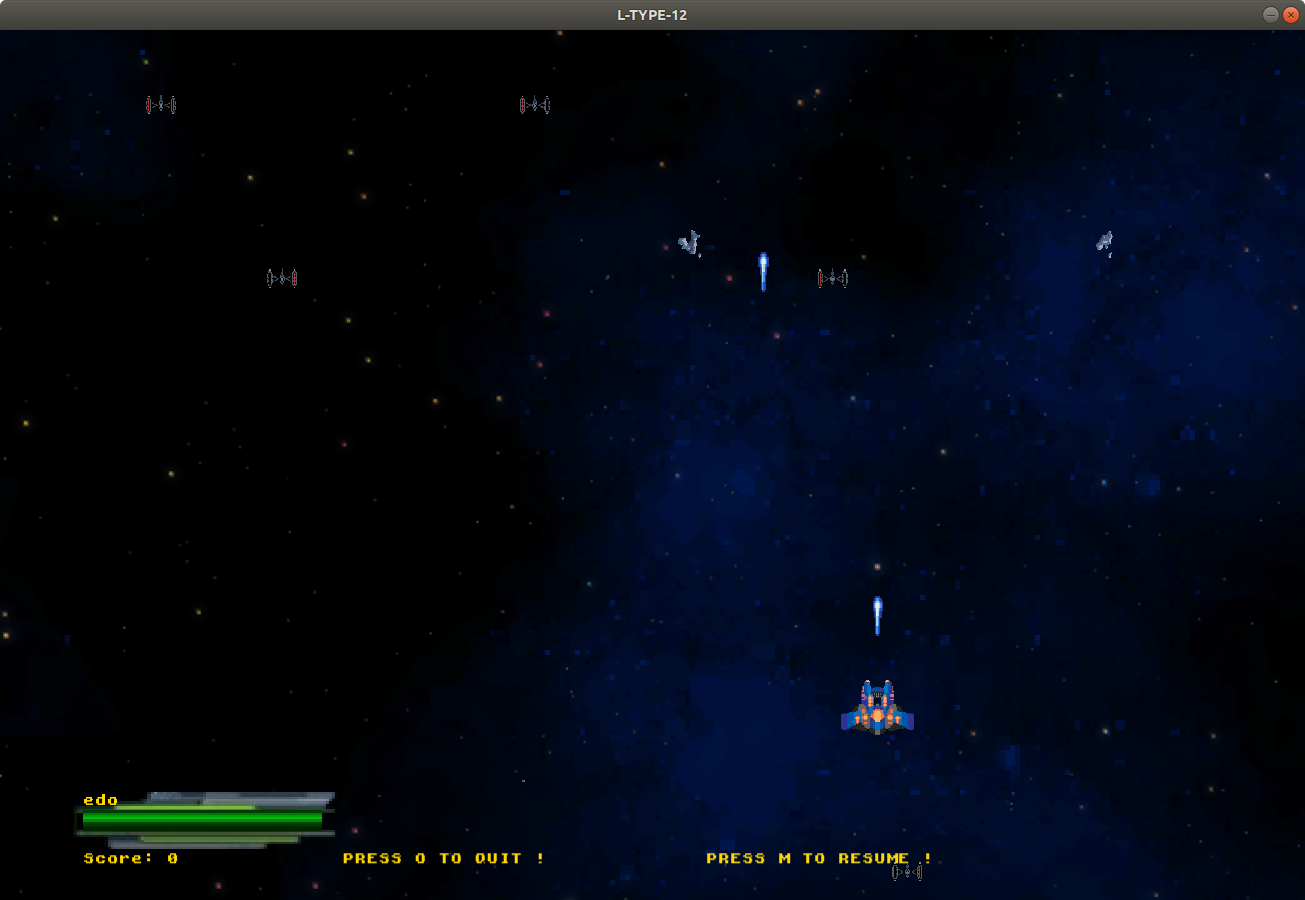
\includegraphics[scale=0.18, angle=0]{Screenshots/SFML/in_game.png}}\\
\subfloat[Winning view Ncurses]{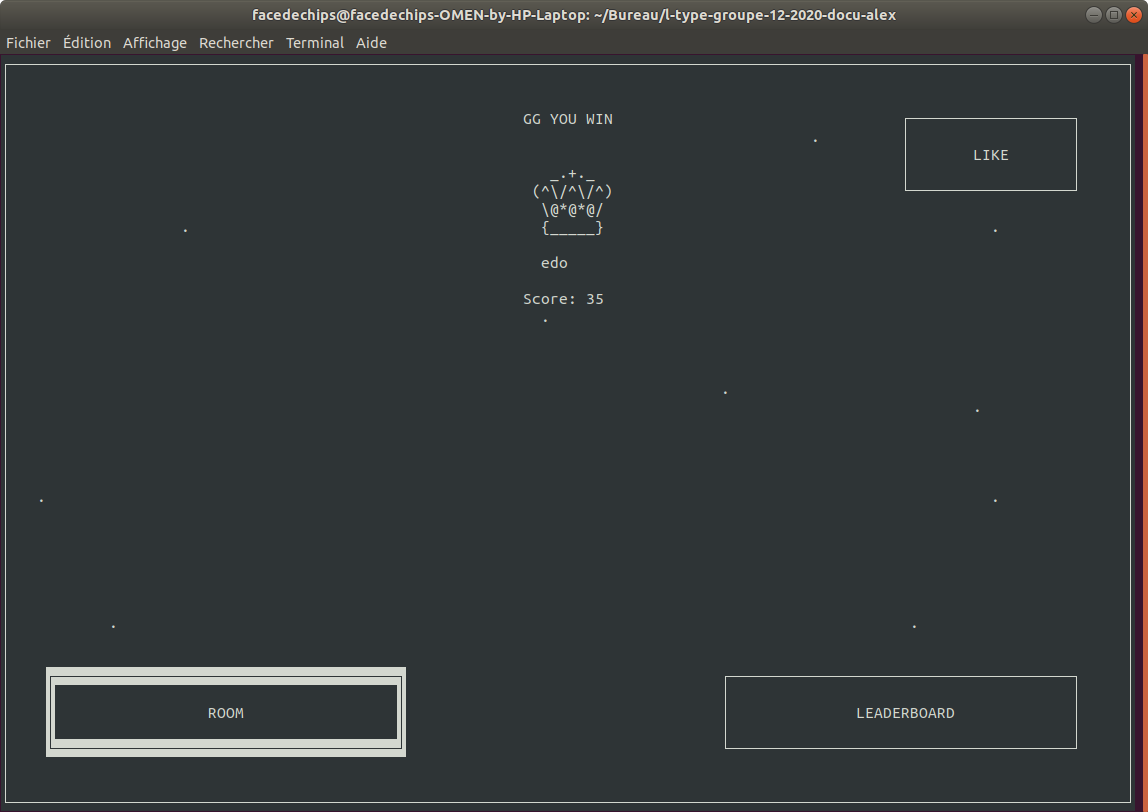
\includegraphics[scale=0.199,angle=0]{Screenshots/NCURSES/win_screen_ncurses.png}}
\subfloat[Winning view SFML]{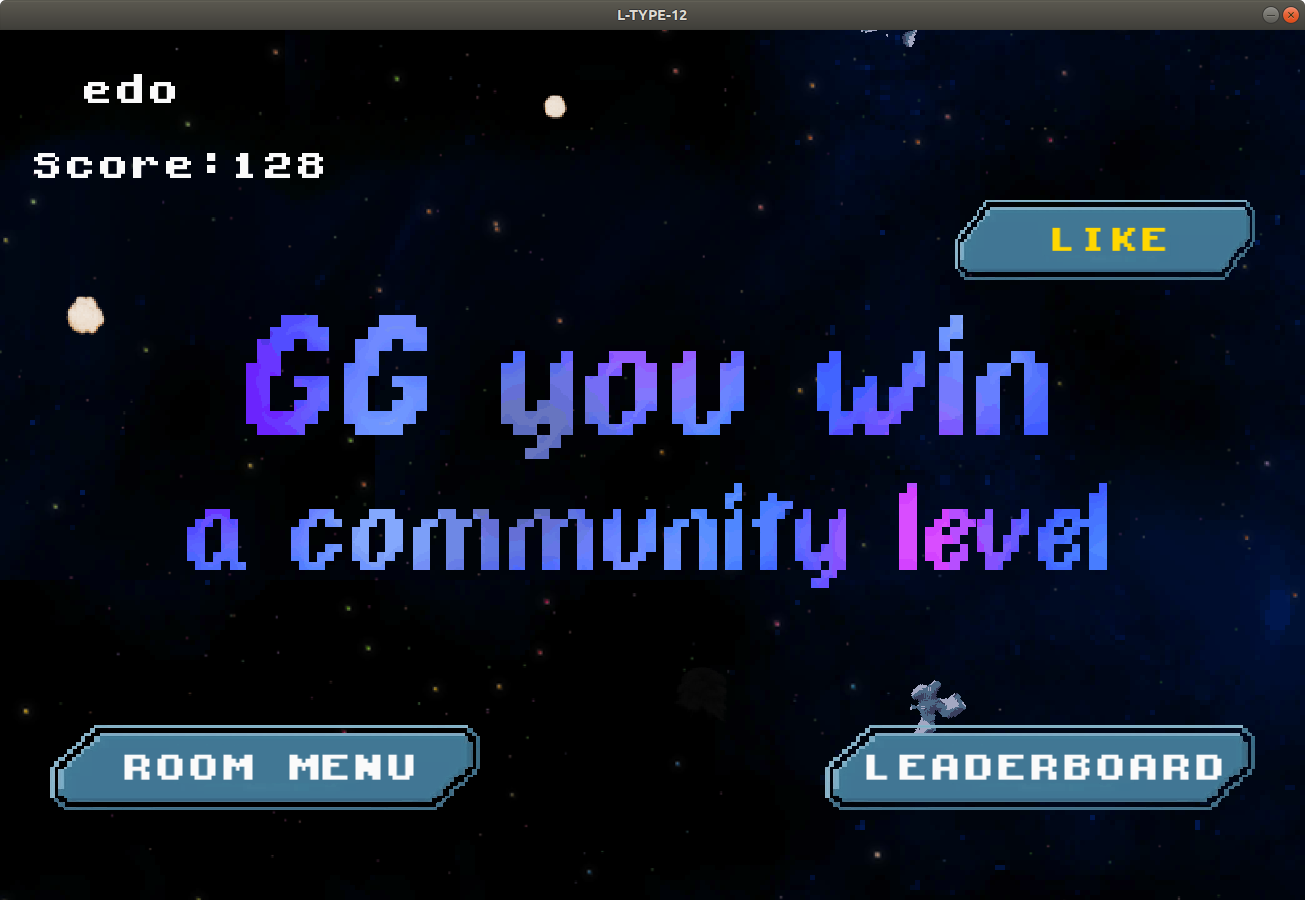
\includegraphics[scale=0.18, angle=0]{Screenshots/SFML/win_screen.png}}\\
\subfloat[Losing view Ncurses]{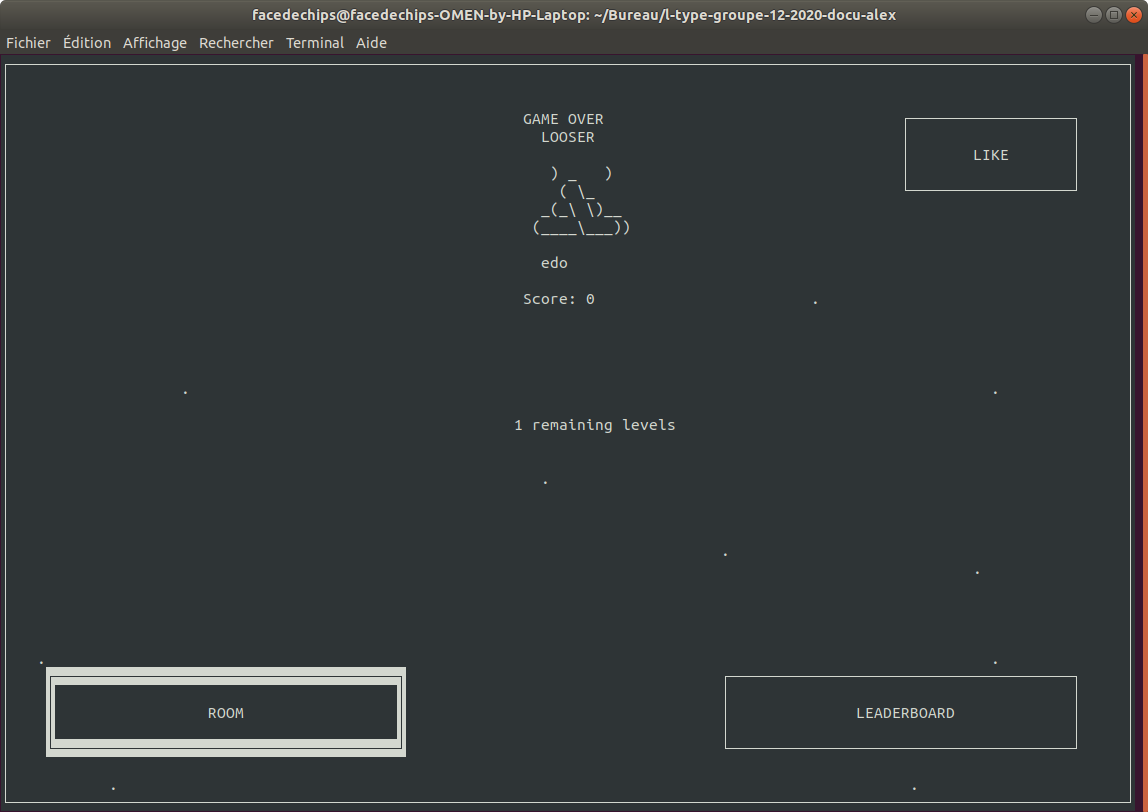
\includegraphics[scale=0.199,angle=0]{Screenshots/NCURSES/lose_screen_ncurses.png}}
\subfloat[losing view SFML]{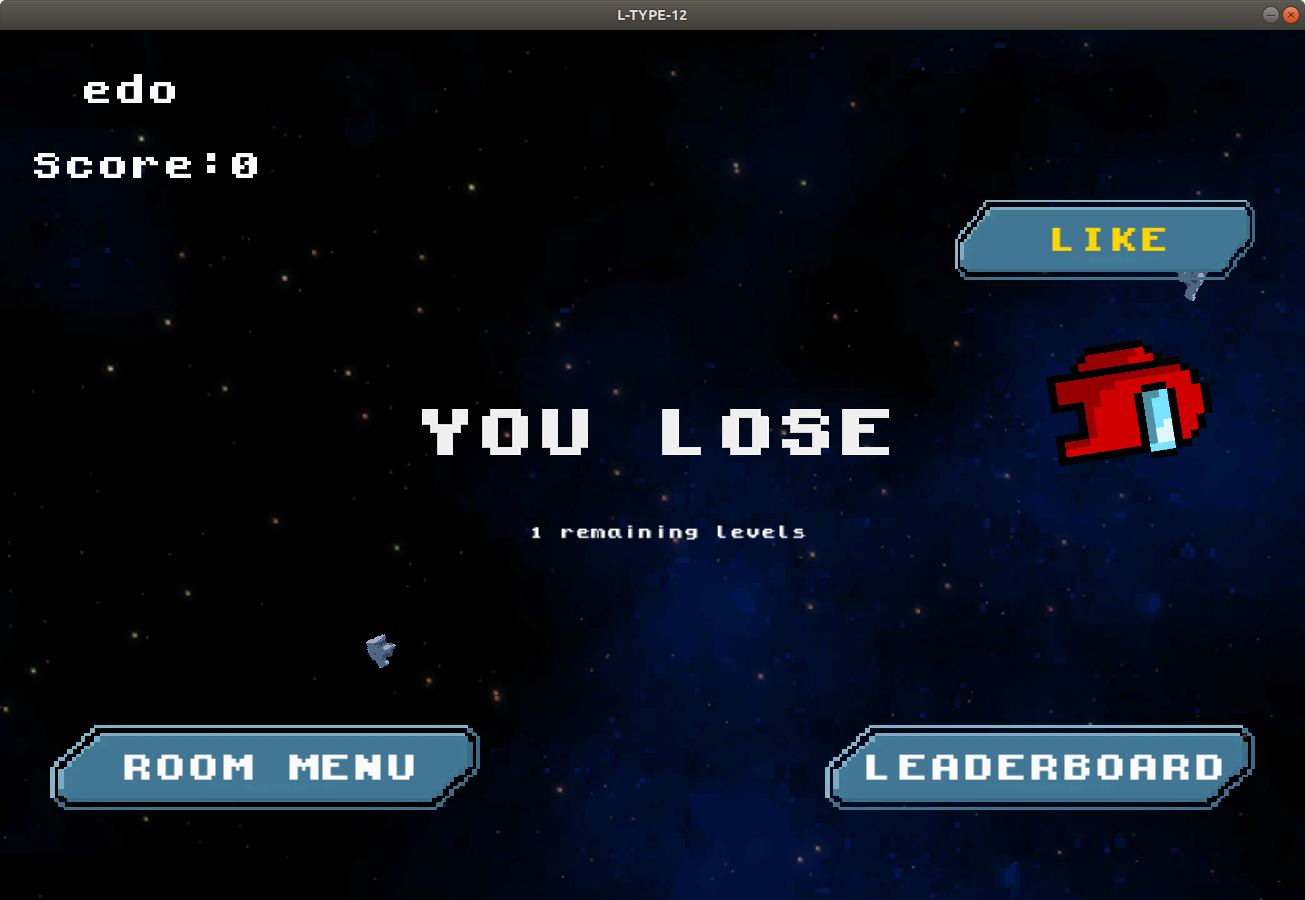
\includegraphics[scale=0.18, angle=0]{Screenshots/SFML/lose_screen.png}}\\
\end{figure}
\begin{figure}[!htbp]
\subfloat[Levels menu SFML]{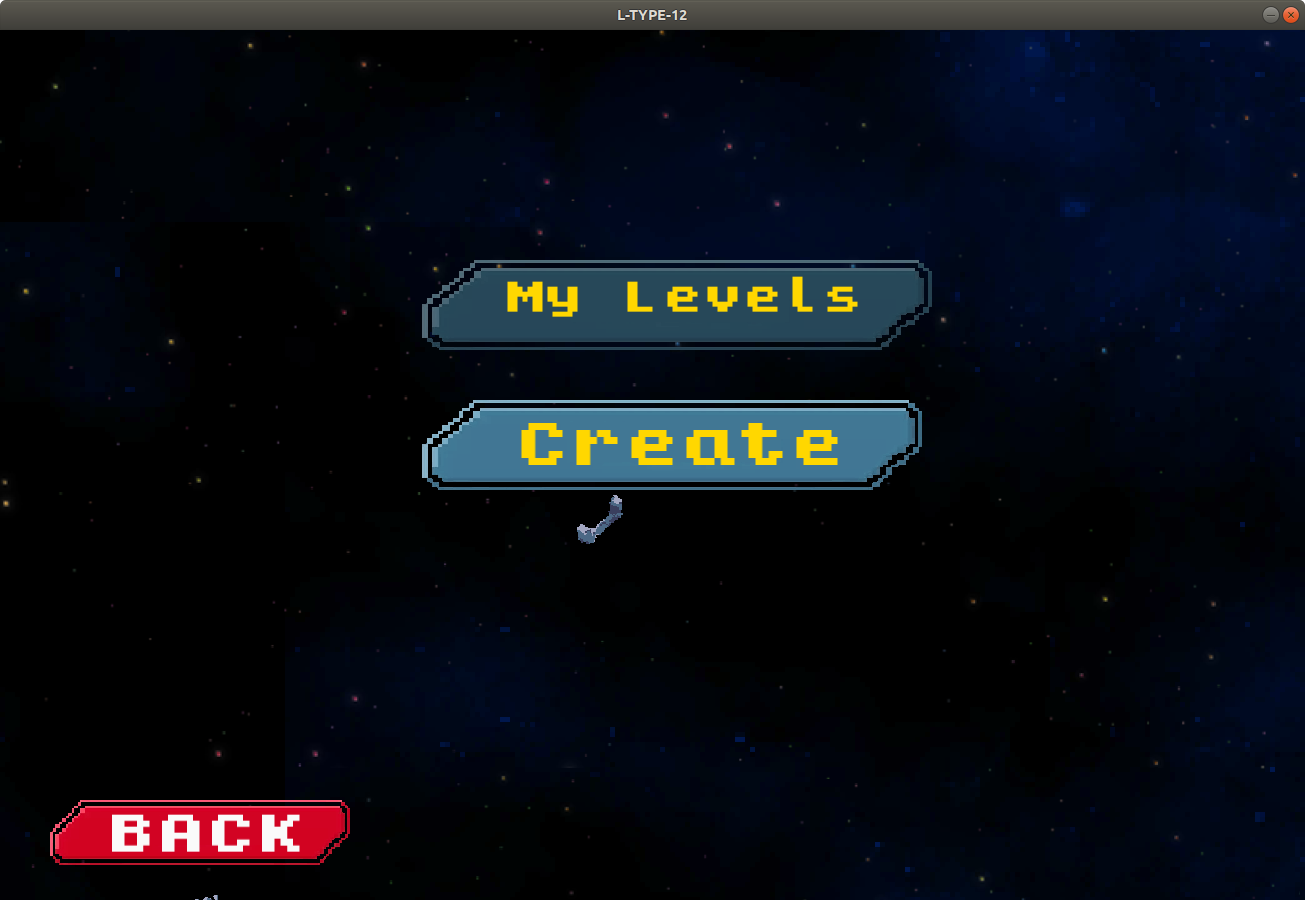
\includegraphics[scale=0.18,angle=0]{Screenshots/SFML/levels_menu.png}}
\subfloat[My levels view SFML]{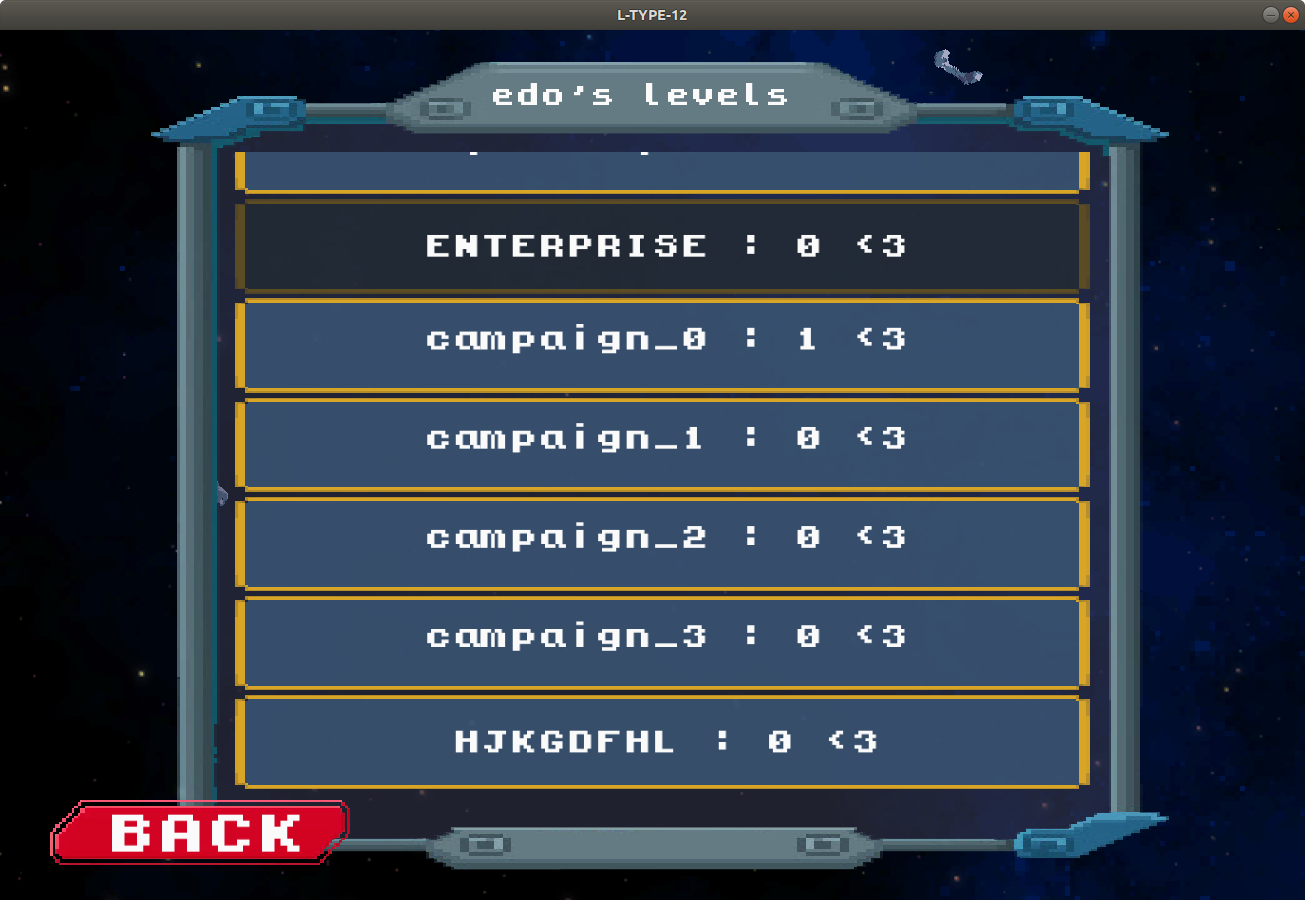
\includegraphics[scale=0.18, angle=0]{Screenshots/SFML/my_levels.png}}\\
\subfloat[Create a level menu SFML]{\includegraphics[scale=0.18,angle=0]{Screenshots/SFML/create_menu.png}}
\subfloat[Editing mode view SFML]{\includegraphics[scale=0.18, angle=0]{Screenshots/SFML/edit_mode_menu.png}}\\
\end{figure}

\begin{figure}[!htbp]
    \centering
    \includegraphics[scale=0.25, angle=0]{assets/title.png}
\end{figure}

\end{document}
